\pdfminorversion=4
\documentclass[11pt,a4paper]{report} 
% Alternativ für doppelseitigen Ausdruck (nur bei > 60 Seiten sinnvoll)
%\documentclass[11pt,a4paper,twoside,openright]{report}

% Deutsch
\usepackage[german]{babel} % deutsch und deutsche Rechtschreibung
\usepackage[utf8]{inputenc} % Unicode Text 
\usepackage[T1]{fontenc} % Umlaute und deutsches Trennen
\usepackage{textcomp} % Euro
\usepackage[hyphens]{url}
% statt immer Ab\-schluss\-ar\-beit zu schreiben
% einfach hier sammeln mit -. 
\hyphenation{Ab-schluss-ar-beit}
% Vorsicht bei Umlauten und Bindestrichen
\hyphenation{Ver-st\"ar-ker-aus-gang}
 % eigene Hyphenations, die für das Dokument gelten
\usepackage{amssymb} % Symbole
\usepackage{enumitem}
\usepackage{tabularx}


%% Fonts, ein kompletter Satz an Optionen
% Times New Roman, gewohnter Font mit ok tt und serifenlos
%\usepackage{mathptmx} 
%\usepackage[scaled=.95]{helvet}
%\usepackage{courier}
% Palatino, mal was anderes, auch mit ok tt und serifenlos
% empfohlen
\usepackage{mathpazo} % Palatino, mal was anderes
\usepackage[scaled=.95]{helvet}
\usepackage{courier}
% New Century Schoolbook sieht auch nett aus (macht auch tt und serifenlos)
%\usepackage{newcent}

% zusätzlich: Default serifenlos mit Helvetica 
% ich kann es nicht mehr sehen...
%\renewcommand{\familydefault}{\sfdefault}

\usepackage{microtype}

% Bilder und Listings
\usepackage{graphicx} % wir wollen Bilder einfügen
\usepackage{subfig} % Teilbilder
\usepackage{wrapfig} % vielleicht doch besser vermeiden
\usepackage{listings} % schöne Quellcode-Listings
% ein paar Einstellungen für akzeptable Listings
\lstset{basicstyle=\sffamily, columns=[l]flexible, mathescape=true, showstringspaces=false, numbers=left, numberstyle=\tiny}
\lstset{language=python} % und nur schöne Programmiersprachen ;-)
% und eine eigene Umgebung für Listings
\usepackage{float}
\newfloat{listing}{htbp}{scl}[chapter]
\floatname{listing}{Listing}

% Seitenlayout
%\usepackage[paper=a4paper,width=14cm,left=35mm,height=22cm]{geometry}
\usepackage[paper=a4paper,width=14cm,height=22cm]{geometry}
\usepackage{setspace}
\linespread{1.15}
\setlength{\parskip}{0.5em}
\setlength{\parindent}{0em} % im Deutschen Einrückung nicht üblich, leider

% Seitenmarkierungen 
\newcommand{\phv}{\fontfamily{phv}\fontseries{m}\fontsize{9}{11}\selectfont}
\usepackage{fancyhdr} % Schickere Header und Footer

\pagestyle{fancy}
\renewcommand{\chaptermark}[1]{\markboth{#1}{}}
\renewcommand{\sectionmark}[1]{\markright{#1}}
\fancyhead[LO]{\phv \nouppercase{\leftmark}}
\fancyhead[RE]{\phv \nouppercase{\rightmark}}
\fancyhead[RO,LE]{\phv \thepage}
\fancyfoot[C]{\ } % Seitenzahl unten nur Kapitel


% Theorem-Umgebungen
\newtheorem{definition}{Definition}[chapter]
\newtheorem{satz}{Satz}[chapter]
\newtheorem{lemma}[satz]{Lemma} % gleicher Zähler wie Satz
\newtheorem{theorem}{Theorem}[chapter]
\newenvironment{beweis}[1][Beweis]{\begin{trivlist}
\item[\hskip \labelsep {\textit{#1 }}]}{\end{trivlist}}
\newcommand{\qed}{\hfill \ensuremath{\square}}

% Inhaltsverzeichnis
\setcounter{tocdepth}{1}
\setcounter{secnumdepth}{2}

% Quellen teilen
\usepackage{bibtopic} 

% Hochschule Logo, noch nicht perfekt
\usepackage{hsrmlogo}

% Spezialpakete
\usepackage{epigraph}
\setlength{\epigraphrule}{0pt} % kein Trennstrich

% damit wir nicht so viel tippen müssen, nur für Demo 
\usepackage{blindtext} 

% Zum Zeigen von Fehlern
\usepackage{soul}
\newcommand*\falsch{\st}

% Links im PDF
\usepackage{hyperref}
\hypersetup{
    colorlinks=true,
    citecolor=black,
    filecolor=black,
    linkcolor=black,
    urlcolor=black
}

% Kommentare
\usepackage{comment} % alle Pakete und Einstellungen	
\usepackage{hyperref}
% Hier anpassen 
\newcommand{\titel}{Entwurf, prototypische Implementierung und Evaluation eines Sicherheitskonzepts für die Authentifizierung und Autorisierung von Fernzugriffen auf eine Automatisierungsanlage}
\newcommand{\kurztitel}{Template Abschlussarbeit}
\newcommand{\autor}{Kevin Sapper}
\newcommand{\datum}{14. Oktober 2014} % Abgabedatum
\newcommand{\ort}{Wiesbaden}
\newcommand{\referent}{Prof.\ Dr.\ Reinhold Kröger}
\newcommand{\korreferent}{Prof.\ Dr.\ Martin Gergeleit}

\newenvironment{conditions*}
  {\par\vspace{\abovedisplayskip}\noindent
   \tabularx{\columnwidth}{>{$}l<{$} @{\ : } >{\raggedright\arraybackslash}X}}
  {\endtabularx\par\vspace{\belowdisplayskip}}

\begin{document}
\shorthandoff{"}
\pagenumbering{Roman}

\begin{titlepage}
  \begin{center}
    % Kopf der Seite
    \hsrmlogo[1]
    \parbox[b]{8cm}{Hochschule RheinMain \\
     Fachbereich Design Informatik Medien \\
     Studiengang Angewandte Informatik}
    \vfill    
    {\LARGE Abschlussarbeit} \\[0.5cm]
    {\large zur Erlangung des akademischen Grades} \\[5mm]
    {\large Bachelor of Science (B.Sc.)} \\[5mm]
    \rule{\textwidth}{1pt}\\[0.5cm]
    {\begin{spacing}{1.15} \huge \bfseries \titel \\ \end{spacing}}
    \rule{\textwidth}{1pt}    
    \vfill    
    \begin{tabular}{ll} % Mitte der Seite
      Vorgelegt von & \autor \\
      am & \datum \\
      Referent & \referent \\
      Korreferent & \korreferent
    \end{tabular}    
    \vfill
  \end{center}
\end{titlepage}
\cleardoublepage


% Erklärung gemäß den Allgemeinen Bestimmungen für Prüfungsordnungen
% der Paragraph schwankt, daher ohne Nennung einer Nummer
\section*{Erklärung gemäß ABPO}
\thispagestyle{empty}
Ich erkläre hiermit,
\begin{itemize}
\item dass ich die vorliegende Abschlussarbeit selbstständig angefertigt,
\item keine anderen als die angegebenen Quellen benutzt,
\item die wörtlich oder dem Inhalt nach aus fremden Arbeiten entnommenen 
  Stellen, bildlichen Darstellungen und dergleichen als solche genau 
  kenntlich gemacht und
\item keine unerlaubte fremde Hilfe in Anspruch genommen habe.
\end{itemize}

\vspace{6em}
\noindent\begin{tabular}{p{0.37\textwidth}p{0.56\textwidth}}
\ort, \datum  & \rule{0.56\textwidth}{0.5pt}\\
              & \makebox[1cm]{\ } \autor
\end{tabular}

\vfill

\section*{Erklärung zur Verwendung der Bachelor Thesis}

Hiermit erkläre ich mein Einverständnis mit den im folgenden 
aufgeführten Verbreitungsformen dieser Abschlussarbeit:

\vspace{1em}
\noindent\begin{tabular}{|p{0.82\textwidth}|c|c|}
  \hline
  \textbf{Verbreitungsform} & \makebox[0.035\textwidth]{\textbf{Ja}} 
                            & \makebox[0.05\textwidth]{\textbf{Nein}} \\\hline
  Einstellung der Arbeit in die Hochschulbibliothek 
                         mit Datenträger   &  & $\times$ \\\hline
  Einstellung der Arbeit in die Hochschulbibliothek  
                         ohne Datenträger  & $\times$ & \\\hline
  Veröffentlichung des Titels der Arbeit im Internet  
                                           & $\times$ & \\\hline
  Veröffentlichung der Arbeit im Internet             
                                           & $\times$ & \\\hline
\end{tabular}

\vspace{6em}
\noindent\begin{tabular}{p{0.37\textwidth}p{0.56\textwidth}}
\ort, \datum  & \rule{0.56\textwidth}{0.5pt}\\
              & \makebox[1cm]{\ } \autor
\end{tabular}
\cleardoublepage

 % Titelseite, Erklärungen, etc.

\begin{comment}
\begin{abstract} 
\end{abstract}
\epigraphhead[70]{\epigraph{Using encryption on the Internet is the equivalent of arranging an armored car to deliver credit card information from someone living in a cardboard box to someone living on a park bench.}{\textit{Gene Spafford}}}
\end{comment}

\tableofcontents
\clearpage 

\pagenumbering{arabic}

\chapter{Einführung} \label{chap:intro}
\epigraphhead[70]{\epigraph{Companies spend millions of dollars on firewalls, encryption and secure access devices, and it’s money wasted, because none of these measures address the weakest link in the security chain.}{\textit{Kevin Mitnick}}}

\begin{itemize}
\item Automatisierungsanlage
\item Entwurf 
\item Sicherheitskonzept
\item Authentifizierung \& Autorisierung
\item Fernzugriff
\item Evaluation
\item prototypische Implementierung
\end{itemize}

\chapter{Grundlagen} \label{chap:basics}

Dieses Kapitel soll die nötigen Grundkenntnisse zum Verstehen dieser Thesis vermitteln. Zunächst wird ein Überblick einer Kälteanlage, aus der Sicht der ECKELMANN AG, vermittelt und wichtige Komponenten und Funktionen erläutert. Danach werden Sicherheitsstandards und Modelle beleuchtet, die das Bundesamt für Sicherheit in der Informationstechnik (BSI) unterstützt, sowie Methodiken zum Vorgehen an eine Bedrohungsanalyse erklärt. Abschließend werden die verbreitetsten Verfahren zur Authentifizierung aufgelistet.

\section{Kälteanlagen}

Die genaue Funktionsweise einer Kälteanlage ist für diese Arbeit nicht relevant. Dennoch gibt es einige Aspekte die ein Sicherheitskonzept beeinflussen können. Ein Aspekt ist die Trägheit. Beim Einsatz von Kälte geschieht nichts in Bruchteilen von Sekunden. Das Kühlen von Waren ist ein langsamer Prozess, ebenso verhält es sich beim Erwärmen. Im folgenden befindet sich eine Auflistung von Komponenten einer Kälteanlage, welche für das Sicherheitskonzept Relevanz haben. Die Beschreibungen der Komponenten einer Kältekälteanlage beziehen sich auf die Firma ECKELMANN und können von Systemen anderer Hersteller abweichen.

\subsection{E*LDS}

E*LDS (Long-Distance-Service) ist die Produktreihe, die von der ECKELMANN AG zur Steuerung und Verwaltung von Kälteanlagen entwickelt wird. Abbildung~\ref{fig:kaelteanlage} zeigt die typische Vernetzung der Komponenten. Diese beinhaltet Verbundsteuerungen zur Kälteerzeugung, Kühlstellenregler zur temperaturgenauen Reglung aller Arten von Kühlmöbeln und Kühlräumen, Funk-Temperatursensoren und den Marktrechner als zentrale Intelligenz einer Kälteanlage \cite{elds}. Über den seriellen Feldbus Controller Area Network (CAN) sind sämtlichen E*LDS-Komponenten der Anlage verbunden. Zusätzlich können über die Modbus-Schnittstelle, welche ebenfalls ein serieller Feldbus ist, Fremdsysteme anderer Hersteller angebunden werden. Für die Vorort-Bedienung kann der Touch-Screen des Marktrechners genutzt werden. Alternativ kann ein PC mit einem CAN-Bus-PC-Adapter verbunden werden und über die Software LDSWin zugreifen. Der Fernzugriff kann über eine Wählverbinung (Modem) oder über VPN, je nach Verfügbarkeit, geschehen. Auch hier wird der Zugriff durch die Software LDSWin ermöglicht.

\begin{figure}[htbp]
\centering
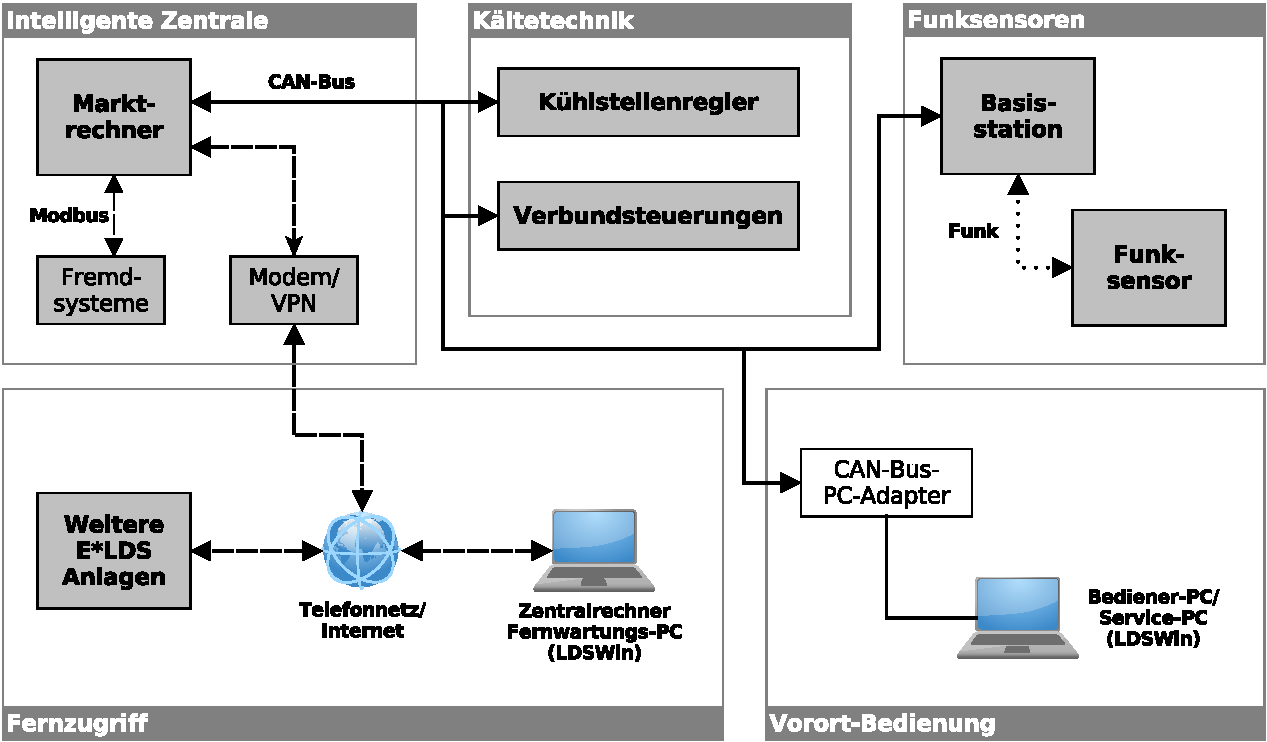
\includegraphics[scale=0.65]{images/kaelteanlage_uebersicht.pdf}
\caption{Übersicht einer Kälteanlage}
\label{fig:kaelteanlage}
\end{figure}

\subsection{Marktrechner} \label{sec:marktrechner} 
Betrachtet man eine Kälteanlage, dann ist der Marktrechner ihr Herzstück. Über den CAN-Bus ist er in der Lage, Komponenten zentral zu parametrieren und zu überwachen. Sämtliche Betriebsdaten und Betriebszustände, Meldungen und Alarme aus der Überwachung werden auf seinem internen Speicher archiviert \cite{elds}.

\paragraph{Hardware} Der Marktrechner verfügt über einen 32-Bit-Prozessor aus der ARM-Prozessorfamilie. Für die persistente Datenspeicherung steht eine fest verbaute SD-Karte zur Verfügung und 256-MB flüchtigen RAM-Speicher sind vorhanden. Als Zentrale Komponente benötigt der Marktrechner einige Schnittstellen für die Kommunikation, diese sind in Abbildung~\ref{fig:marktrechner_interfaces} zu sehen. Über den Ethernet-Port ist der Marktrechner mit dem Unternehmensnetzwerk verbunden, darüber kann die Fernwartung erfolgen. Über die drei RS-232 COM-Schnittstellen können ein PC vor Ort angeschlossen werden, die Fernwartung via Modem erfolgen, das M-Bus-Gateway zur Verbrauchsdatenerfassung verbunden werden oder Sonderfunktionen, beispielsweise Gebäudeleittechnik oder sonstige Fremdsysteme, integriert werden. Über die RS-485 COM-Schnittstelle können Modbus-Regler hinzugefügt werden. Die USB-Anschlüsse sind für zukünftige Benutzung vorgesehen. Einer der beiden CAN-Bus-Anschlüsse wird benutzt, um mit den E*LDS-Komponenten zu kommunizieren. Der zweite Anschluss ist ebenfalls für zukünftige Benutzung vorgesehen und über die zwei Digitaleingänge können entweder Alarme entgegengenommen oder Energiezähler ausgelesen werden. Die Benutzerinteraktion findet über ein 7-Zoll Touch-Display statt.

\begin{figure}[htbp]
\centering
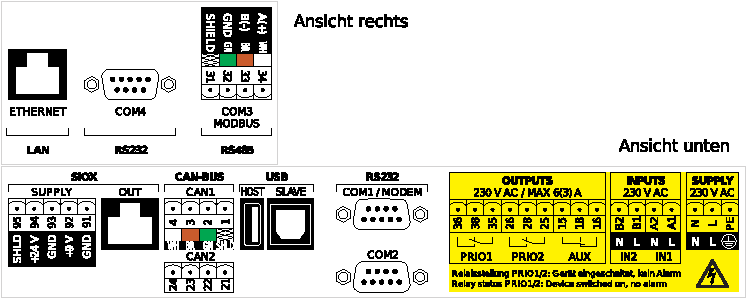
\includegraphics[scale=1.1]{images/CI4000_Hardware_Sticker.pdf}
\caption{Schnittstellen des Marktrechners}
\label{fig:marktrechner_interfaces}
\end{figure}

\paragraph{Software}

Das Betriebssystem auf dem Marktrechner ist eine eigene Linux-Distribu\-tion, welche mit der Software ptxdist der Pengutronix e.K. erstellt wird. Ptxdist bringt einige hundert Module und Bibliotheken mit. Darunter sind etwa der leichtgewichtige HTTP-Server lighttpd, der SSH-Server openssh oder das Synchronisierungstool rsync. Mit ein wenig Konfigurationsaufwand können auch eigene Module hinzugefügt werden. Über eine Toolchain, die ebenfalls von der Pengutronix e.K. geliefert wird, kann eine sehr schlanke Distribution für viele Prozessorarchitekturen erzeugt werden, die auf den eigenen Software-Stack zugeschnitten ist. Die eigenen Softwaremodule sind in C++ geschrieben und nutzen das Qt-Framework. 

\paragraph{Funktionen} \label{para:architektur}

Alle Daten und Meldungen, die der Marktrechner sammelt und aufbereitet, müssen ausgewertet werden. Die 24-Stunden-Überwachung vor Ort, durch einen Mitarbeiter des Eigentümers, ist nicht wirtschaftlich. Auch das fachliche Wissen zur Betreuung einer Kälteanlage ist beim Endkunden nicht vorhanden. Deshalb übernehmen heutzutage großteils Fernservice-Zentralen (FSZs) die Überwachung von Kälteanlagen. FSZs haben in der Kältetechnik ausgebildete Mitarbeiter, die Daten und Meldungen der Marktrechner interpretieren können. Der Marktrechner kann aus der Ferne über eine Ethernet- oder eine Modem-Verbindung erreicht werden. Letztere wird, aufgrund ihres aussterbendes Charakters, an dieser Stelle nicht weiter betrachtet. Für den Zugriff auf die Ethernet-Schnittstelle sind Fernservice-Zentralen über VPN mit einem oder mehreren Unternehmensnetzwerken ihrer Kunden verbunden (Abbildung~\ref{fig:current_setup}). Über dieses können die Marktrechner erreicht werden. Auf diese Weise kann eine einzige Fernservice-Zentrale Tausende Marktrechner überwachen. Der Marktrechner fungiert dabei als Server, das heißt, Daten und Meldungen müssen aktiv von einer Fernservice-Zentrale abgeholt werden. Ist aus den abgeholten Daten ersichtlich, dass ein Fehler in der Anlage aufgetreten ist, kann die Fernservice-Zentrale entweder direkt eingreifen oder einen Monteur zum betreffenden Kunden schicken, der die Anlage instand setzt.

\begin{comment}
@startuml images/problemfeld.svg
skinparam monochrome true
skinparam dpi 150

package "Unternehmensnetzwerk A" as UA {
  [Marktrechner 1]
  [Marktrechner 2]
  [...]
  [Marktrechner n]
}

package "Unternehmensnetzwerk B" as UB {
}

package "Unternehmensnetzwerk C" as UC {
}

cloud VPN {
}

[Fernservice-Zentrale] -down- VPN
VPN -down- UA
VPN -left- UB
VPN -right- UC
UA - [Marktrechner n]
UA - [...]
UA - [Marktrechner 2]
UA - [Marktrechner 1]

@enduml
\end{comment}

\begin{figure}[htbp]
\centering
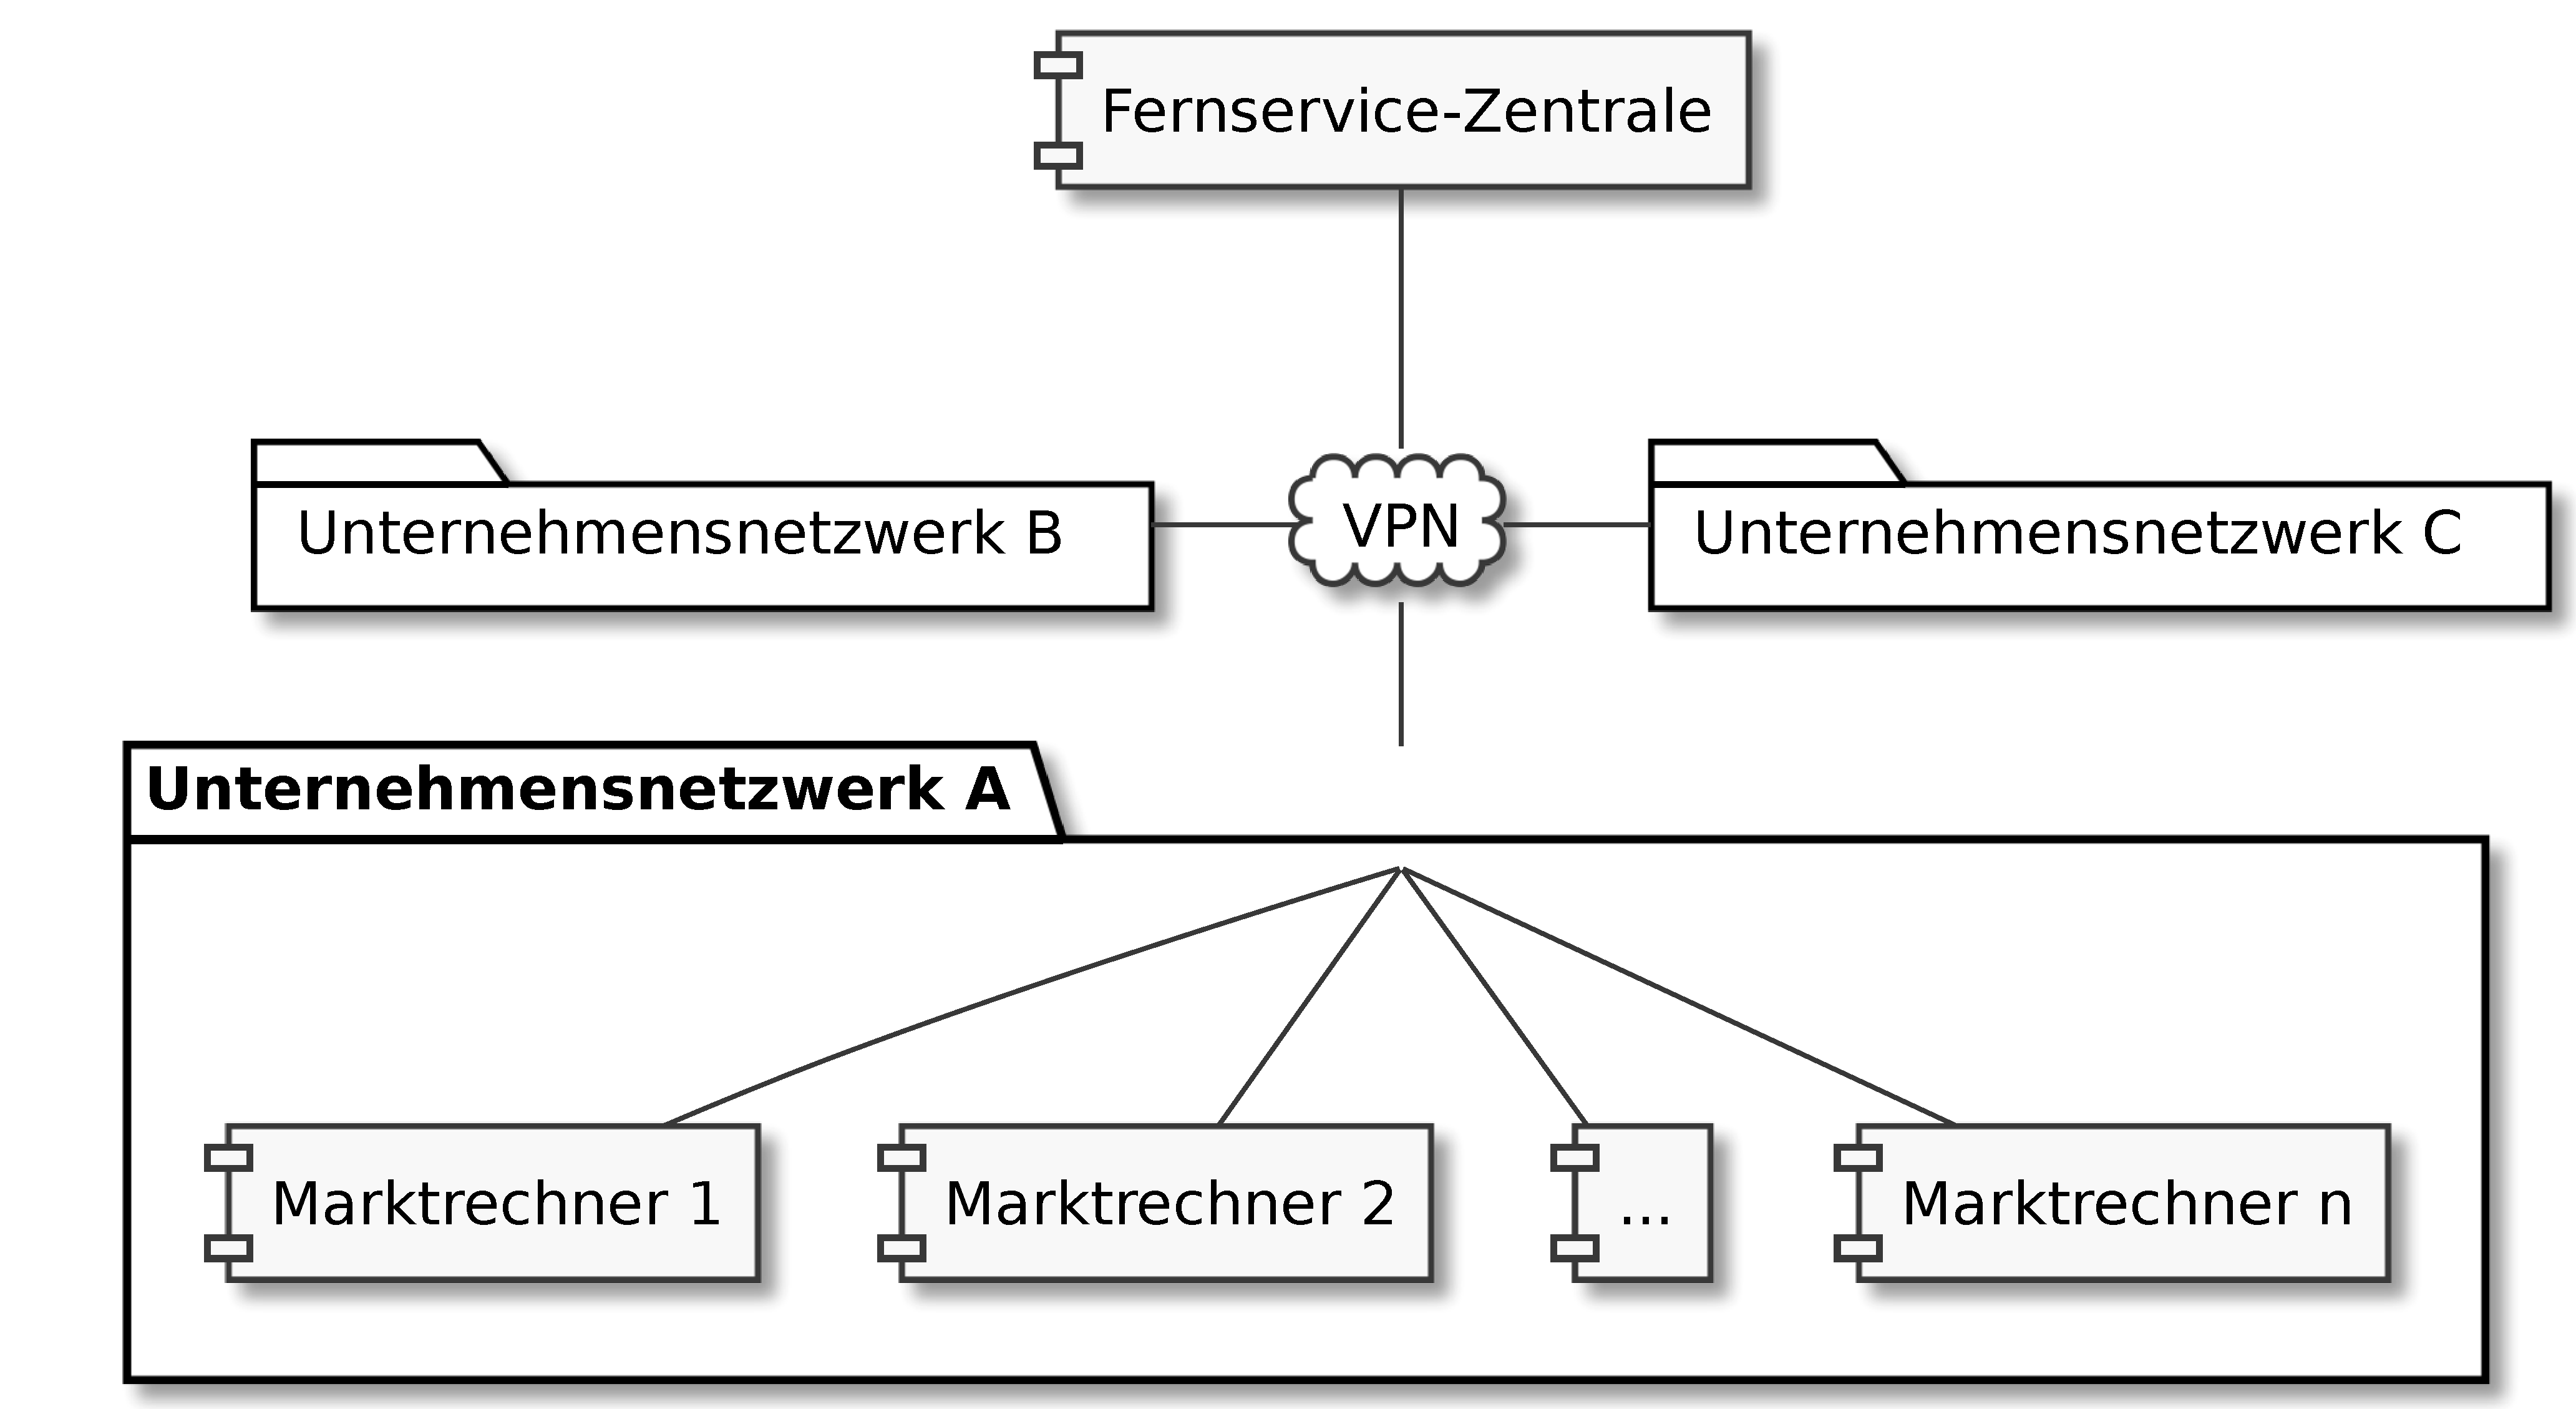
\includegraphics[scale=0.19]{images/problemfeld.pdf}
\caption{Aktuelle Architektur}
\label{fig:current_setup}
\end{figure}

Beim Einsatz von VPN ist die Kommunikation von der Fernservice-Zentrale bis zum Unternehmensnetzwerk abgesichert. Im Lokal Area Network (LAN) des Unternehmens ist der gesamte Datenverkehr zu und von den Marktrechnern allerdings unverschlüsselt. Aktuell gibt es zwei Arten von Datenverkehr zwischen Marktrechner und FSZ, zum einen über das proprietäre Protokoll des Herstellers und zum anderen über Webservices auf Basis von einfachen XML-RPCs.

\subsection{RestGateway} 

Das RestGateway ist die Neuauflage des XML-RPC. Es wurde vom Author dieser Thesis im Rahmen des vor der Thesis absolvierten Praktikums entwickelt. Es basiert auf dem Representational State Transfer (REST) Konzept zur Entwicklung von Webanwendungen. REST ist keine explizite Norm, sondern bezeichnet vielmehr die Idee, dass eine URL genau einen Ressource oder eine Liste von Ressourcen als Ergebnis einer serverseitigen Aktion liefert \cite{wiki_rest}. REST nutzt Standard HTTP-Befehle, um lesend und schreibend auf Ressourcen zuzugreifen. Zur Zeit sind ausschließlich lesende Zugriffe implementiert, welche über URLs abgerufen werden können. Diese Aufrufe liefern interpretierte Inhalte im XML- oder JSON-Format. Zudem gibt es eine generische Schnittstelle, welche als Proxy für CAN-Nachrichten fungiert, dadurch können beliebige CAN-Nachrichten über HTTP/S gesendet werden, auch solche, die schreibend auf das System zugreifen. Das RestGateway bietet keinerlei Mechanismus für die Authentifizierung und Autorisierung. Eine Erweiterung wäre auf Basis dieser Arbeit vorgesehen. Das RestGateway kann in zwei Ausführungen installiert werden, entweder als Modul auf dem Marktrechner (Abbildung~\ref{fig:rest_intern}), oder auf einem externen Server (Abbildung~\ref{fig:rest_extern}). Die unterschiedlichen Ausführungen werden durch das LanGateway-Modul des Marktrechners ermöglicht. Dieses ist eine TCP-Schnittstelle, welche als Proxy zwischen TCP-Netzwerk und CAN-Netzwerk fungiert. Über TCP werden die CAN-Nachrichten, ohne Daten-Wrapper wie XML, als Bytestrom übertragen.

\begin{figure}[htbp]
\centering
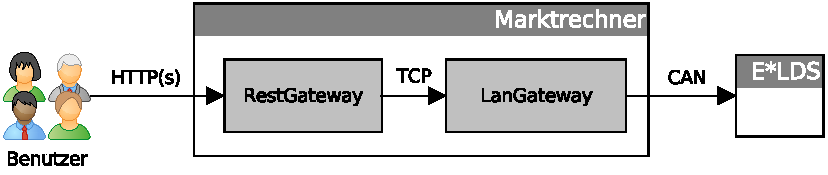
\includegraphics[scale=0.7]{images/RestGateway_intern.pdf}
\caption[]{RestGateway als Marktrechner-Modul}
\label{fig:rest_intern}
\end{figure}

Intern ist das RestGateway ein Wrapper über dem LanGateway, welches interpretierte Inhalte in einem menschenlesbaren Format liefert.

\begin{figure}[htbp]
\centering
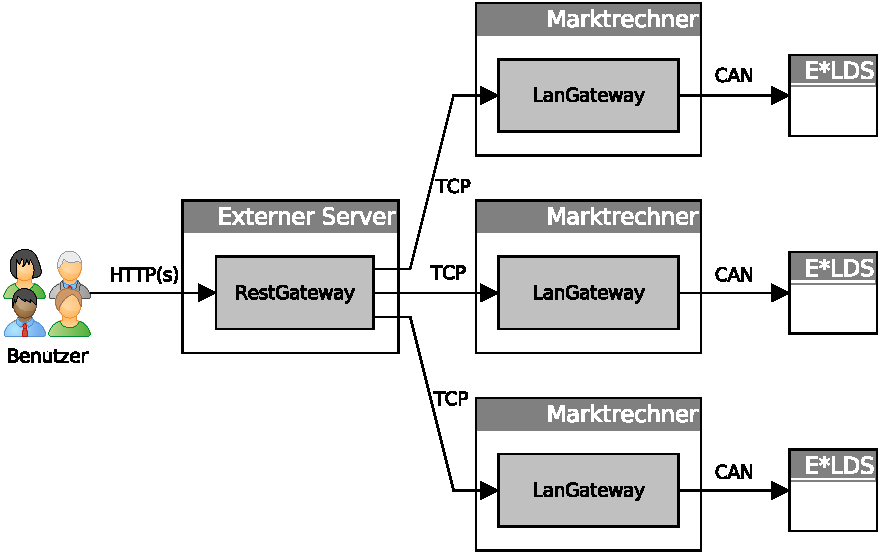
\includegraphics[scale=0.7]{images/RestGateway_extern.pdf}
\caption[]{RestGateway auf externen Server}
\label{fig:rest_extern}
\end{figure}

Extern bietet das RestGateway die Möglichkeit, über die REST-Schnittstellen verschiedene Marktrechner abzufragen. Dieses Feature ist vor allen Dingen für Fernservice-Zentralen interessant, da dort viele Marktrechner verwaltet werden (vgl. \ref{para:architektur}). Des Weiteren können über diesen Weg neue Funktionen ohne große Installationsaufwände erprobt werden, denn es wird kein aufwendiges Update der Marktrechner-Software notwendig. Ein solches Update ist deshalb so aufwendig, da zahlreiche Marktrechner aktualisiert werden müssen und dies jeweils vor Ort geschehen muss, was zu erheblichen Kosten führt.

\subsection{Alarmmanagement} 

Das Alarmmanagement beschreibt die Reaktion auf Fehlfunktionen einer Kälteanlage. Jede Kälteanlage ist anders aufgebaut und nutzt unterschiedliche Kühlmöbel, deshalb müssen Alarme speziell konfiguriert werden. Ein Alarm trifft eine Aussage über den Betriebszustand der Kälteanlage, beispielsweise soll ein Alarm ausgelöst werden, wenn die Temperatur in einem Kühlmöbel einen bestimmten Grenzwert überschreitet beziehungsweise unterschreitet. Damit auf Alarme reagiert werden kann, werden Anlagen überwacht. Dazu können Alarme entweder von Fernwarten in bestimmten Intervallen, etwa alle 15 Minuten, ausgelesen werden, oder alternativ können Alarme durch das System selbstständig, per E-Mail- oder per SMS-Benachrichtigung, versenden werden. Zusätzlich ist im Marktrechner eine Hupe installiert, die auf Fehlfunktionen vor Ort aufmerksam macht. 

\subsection{Offline-Konfiguration} 

Eine Offline-Konfiguration ist eine an den Markt angepasste Konfiguration der Kälteanlage, welche vor Inbetriebnahme erstellt wurde. Ein Teil ist unter anderem die genaue Parametrierung der Kühlgeräte und Kühlmöbel, unter Berücksichtigung der darin zu lagernden Waren. Ein weiterer Teil der Offline-Konfiguration sind auch die Alarme. Die technischen Konfiguration des Marktrechners, beispielsweise Netzwerkkonnektivität, Internetzugang oder Berechtigungsnachweise, sind aktuell nicht in der Offline-Konfiguration enthalten.

\section{Sicherheit} \label{sec:security_conzept}

Viele Sicherheitssysteme heutzutage sind \textit{"sicher"}, da sich niemand die Mühe gemacht hat, diese anzugreifen \cite[s.~0]{gutmann}. Ein Großteil der Probleme von Sicherheitskonzepten entsteht, weil die Anforderungen an Sicherheit erst im Nachhinein aufkommen, wenn das eigentliche System schon fertig konzipiert oder implementiert ist. Meist wird dann versucht, die Sicherheit irgendwie noch an das System anzuheften. Sicherheit wirkt in diesen Fällen oft wie ein fünftes Rad am Wagen, wodurch Systeme entstehen, die für den Anwender extrem mühselig zu benutzen sind. Dabei sollte berücksichtigt werden, dass Benutzer Sicherheit lieber ausschalten oder umgehen, als sich damit auseinanderzusetzen \cite[s.~5]{gutmann}. Bevor man über potentielle Eigenschaften eines Sicherheitssystems nachdenkt, sollte man daher zunächst das Umfeld betrachten, in welchem das System eingesetzt werden soll \cite[s.~4]{gutmann}. Wenn heutzutage über Sicherheit diskutiert wird, wird meistens ausschließlich über Kryptographie gesprochen. Auch wenn Kryptographie Hauptbestandteil jedes Sicherheitssystems ist, ignorieren praktisch alle Angriffe die Kryptographie und attackieren den Weg wie diese genutzt wird \cite[s.~1]{gutmann}. Ein bekanntes Beispiel ist der Heartbleed-Bug\footnote{(Q2/2014) weitere Informationen unter http://heartbleed.com}, der eine Lücke in der Heartbeat-Implementierung der OpenSSL Bibliothek ausnutzt, um sich Zugriff auf den privaten Kommunikationsschlüssel zu verschaffen. Es ist daher nicht sinnvoll, die kryptographischen Mittel auszureizen, wenn kein Angreifer diese versucht zu attackieren. Zudem wird durch Verschlüsselung das Hauptproblem eines Sicherheitssystems, nämlich \textit{"Vertrauen"}, nur unzureichend betrachtet. Das Problem, die Authentifizierung effizient und zuverlässig über einen einzigen Kommunikationskanal zu lösen, besteht bis heute, ohne dass es eine etablierte Lösung dafür gibt (vgl.~\ref{sec:auth_modells}). 

Teil des Sicherheitskonzeptes dieser Arbeit wird es sein, dieses Authentifizierungsproblem auf geeignete Weise zu berücksichtigen, ohne dass durch den Einsatz einer bestimmten Technologie im Extremfall enorme Kosten entstehen können. Ein solcher Extremfall würde eintreten, wenn beispielsweise durch die Kompromittierung der Software oder Hardware alle Berechtigungsnachweise manuelle ausgetauscht werden müssen.

\subsection{Sicherheitsstandards} \label{sec:sec_standard}

Sicherheitsstandards sind von staatlichen Behörden oder Organisationen (DIN, ISO) festgelegte Anforderungen an sichere Systeme. Die Standards klassifizieren sichere Systeme anhand von Stufen, je höher die Stufe, desto mehr Aufwand ist nötig, um diesen zu erreichen. Der erste Sicherheitsstandard mit hohem Verbreitungsgrad war der Trusted Computer System Evaluation Criteria (TCSEC) und wurde 1983 vom amerikanischen Department of Defense (DoD) veröffentlicht. Vor 1990 veröffentlichten auch andere Regierungen, unter anderen Kanada, Westdeutschland, Frankreich und Großbritannien eigene Standards. Da diese Standards nur in den jeweiligen Ländern verwendet wurden und es keine internationale Anerkennung gab, hat die EU 1990 den Standard Information Technology Security Evaluation Criteria (ITSEC) für europäische Staaten veröffentlicht. Dieser Standard war jedoch auf Europa begrenzt, weshalb 1996 mit den Common Criteria for Information Technology Security Evaluation (CC) ein weltweit anerkannter Standard gebildet wurde. Beteiligte Staaten an den CC sind Australien/Neuseeland, Kanada, Frankreich, Deutschland, Japan, Niederlande, Spanien, Großbritannien und die USA.

\subsubsection{Common Criteria for Information Technology Security Evaluation}

Die Common Criteria for Information Technology Security Evaluation sehen sieben Sicherheitsstufen für die Klassifizierung vor. Diese Evaluation Assurance Level (EAL) sind bis Stufe 4 international anerkannt. Der Aufwand, der für die Stufen 5-7 betrieben werden muss, ist allerdings so umfangreich, dass er nur für eine Minderheit an Unternehmen in Frage kommt. Die aktuelle Version 3.1. Release 4 wurde im September 2012 veröffentlicht. Alle weiteren Erläuterungen beziehen sich auf diese Version und sind den Quellen \cite{ccp1, ccp2, ccp3, bsi_ccguide} entnommen.

\paragraph{Klassifizierung}

Die Klassifizierung ist in Abbildung~\ref{fig:eal_sum} gezeigt. Die sieben EAL-Stufen haben Anforderungen in sechs Assurance-Klassen (Assurance class), wobei eine Assurance-Klasse aus mindestens einer Assurance-Familie (Assurance Family) besteht. Die Familien sind dabei selbst in Stufen eingeteilt. Die Anzahl der Stufen in den Familien ist von Familie zu Familie unterschiedlich. Beispielsweise fordert EAL-3 aus der Klasse "Tests" in der Familie "Analyse der Abdeckung" (ATE\_COV) die Stufe 2 und EAL-7 aus der gleichen Familie Stufe 3. Einige Familien sind erst ab höheren EAL Stufen erforderlich. 

\begin{figure}[htb]
\centering
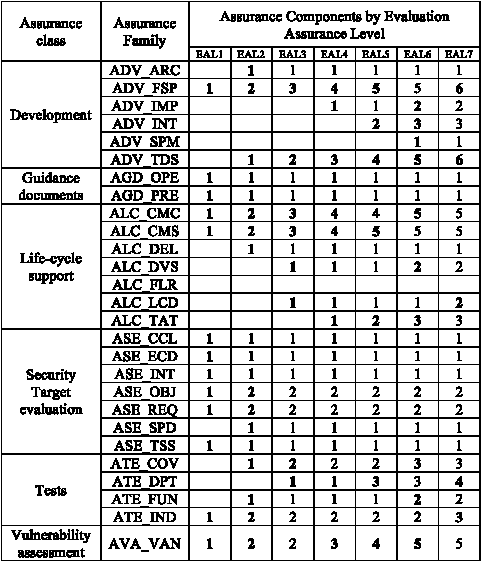
\includegraphics[scale=1.2]{images/cc_eal_table.pdf}
\caption[]{Evaluation assurance level Zusammenfassung aus \cite{bsi_ccguide}}
\label{fig:eal_sum}
\end{figure}

\paragraph{Vorgehen}

Für die Zertifizierung sehen die CC zwei Möglichkeiten vor: Zum einen kundengetrieben, zum anderen entwicklergetrieben. Bei der ersten Möglichkeit stellt der Kunde seine Anforderungen an Hardware und Software in einem Protection Profile (PP) zusammen. Anhand dessen kann er das im PP beschriebene System oder Produkt in Auftrag geben. Alternativ kann er anhand dessen existierende Lösungen evaluieren. Die Entwickler müssen mit dem Security Target (ST) nachweisen, dass das entwickelte System/Produkt den Anforderungen aus dem Protection Profile genügt. Mit Hilfe von PP und ST kann von einer unabhängigen Prüfstelle zertifiziert werden, dass die Inhalte und die Umsetzung der beiden Dokumente der Wahrheit entsprechen.

\begin{figure}[htbp]
\centering
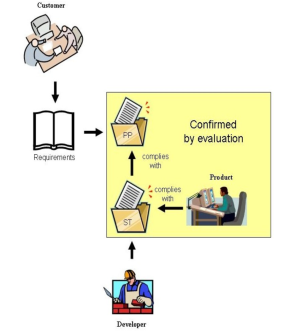
\includegraphics[scale=1.8]{images/cc_prozess.pdf}
\caption[]{Common Criteria Vorgehen aus \cite{bsi_ccguide}}
\label{fig:cc_prozess}
\end{figure}

Die Inhalte aus Protection Profile und Security Target sind großteils identisch, wobei das ST zusätzlich konkrete beschreibt, wie die Anforderungen des PP erfüllt wurden. Bei der zweiten Möglichkeit fällt der Kunde weg und die Entwickler schreiben ein Security Target, um von einer Prüfstelle ein Zertifikat zu erhalten, welches als Qualitätsmerkmal ihres Produktes beworben werden kann. Die Beschreibung des erfüllen von Anforderungen ist stark produkt- bzw. systemabhängig und wird daher nicht weiter erläutert.

\paragraph{Protection Profile}

Die Erstellung eines Protection Profiles wird im folgenden mit der Erklärungs-Methode beschrieben, welche aus insgesamt sechs Teilen besteht. Das Vorgehen dieser Methode soll vor allen Dingen Verständlichkeit beim Leser schaffen. Die Informationen darüber stammen aus \cite{bsi_ccguide}.
\begin{enumerate}
\item Als erstes werden Konformitätsansprüche beschrieben. Darunter fallen Verweise auf die Version des CC, abhängige Protection Profile und welche EAL-Pakete genutzt werden. Abschließend wird noch beschrieben, wie strikt sich PPs und STs, die diese PP benutzen wollen, an die Inhalte halten müssen.
\item Im zweiten Schritt werden die Sicherheitsprobleme definiert. Dabei werden in Bezug auf das zu evaluierende Ziel (Target of Evaluation--TOE) Gesetze, sonstige Regulierungen und Bedrohungen analysiert. Bei den Bedrohungen liegt der Fokus auf den zu schützenden Gütern.
\item Im dritten Schritt werden zu den Sicherheitsproblemen aus dem vorherigen Schritt abstrakte, präzise Lösungsvorschläge erarbeitet. Dabei soll sich auf das "Was" konzentriert werden und nicht beschrieben werden, "Wie" etwas zu lösen ist. Im CC-Kontext heißen diese Lösungsvorschläge Security Objects. 
\item Im vierten Schritt wird für jedes Security-Object ein detailliertes Security Functional Requirement (SFR) erfasst. Die SFRs werden dabei an relevante, thematische Gruppen gekoppelt, welche im CC-Standard vorgegeben sind. Die Beschreibung als SFR umfasst die Beteiligten, die Informationsflüsse, die Operationen und die Daten. Mit Abschluss dieses Schrittes sind die Sicherheitsanforderungen an das System beziehungsweise Produkt festgelegt. 
\item Im Schritt fünf werden Security Assurance Requirements (SAR) festgelegt. Diese sagen aus, wie das TOE zu evaluieren ist und ermöglichen dadurch den Vergleich von zwei Security Targets.
\item Die Einleitung kommt zum Schluss, sie fasst die Inhalte des PP in Prosa zusammen und führt den Leser in die Thematik ein.
\end{enumerate}

\subsection{Sicherheitsmodell}

Ein Sicherheitsmodell bietet einen Leitfaden zur Erstellung eines Sicherheitskonzeptes. Ein ganzheitliches Modell stellt das Bundesamt für Sicherheit in der Informationstechnik (BSI) in seinem IT-Grund\-schutz vor.

\subsubsection{BSI-Sicherheitsmodell}

Folgende Ausführungen sind den BSI IT-Grundschutzempfehlungen entnommen \cite{bsi_grundsch1,bsi_grundsch2,bsi_grundsch3,bsi_grundsch4}.
Das Ziel des Grundschutzes ist das Erreichen eines mittleren, angemessenen und ausreichenden Schutzniveaus für IT-Systeme \cite{wiki_itgrundschutz}. Zu diesem Zweck stellt das BSI ein Modell zur Entwicklung von Sicherheitskonzepten zur Verfügung. In Abbildung~\ref{fig:bsi_sicherheit} sind die empfohlenen Schritte gezeigt. 

Schritt eins verlangt die Erfassung aller Komponenten im Geltungsbereich. Dazu soll das Zusammenspiel zwischen Geschäftsprozessen und Anwendungen herausgearbeitet werden. Als nächstes soll der Schutzbedarf der Komponenten aus Schritt eins ermittelt werden. Der ermittelte Schutz soll gemäß der eingesetzten Informationstechnik ausreichend beziehungsweise angemessen sein. Anhand dieser Informationen werden für die Zielobjekte aus Strukturanalyse und Schutzbedarf Bausteine aus dem IT-Grundschutz gewählt. Der anschließende Basis-Sicherheitscheck soll das aktuelle Sicherheitsniveau einschätzen und liefert als Ergebnis eine Liste der relevanten Maßnahmen und ihren Umsetzungsstatus "entbehrlich", "ja", "teilweise" oder "nein". Dafür sollen Gefährdungenkataloge und Maßnahmenkataloge des BSI genutzt werden. In Schritt vier wird geprüft, ob die Standard-Sicherheitsmaßnahmen ausreichend sind, was für die meisten typischen Geschäftsfelder der Fall sein sollte. Sollten erweitere Sicherheitsmaßnahmen nötig werden, müssen für diese Risikoanalysen durchgeführt werden. Bei den Standard-Sicherheitsmaßnahmen ist dies bereits durch die IT-Grundschutz-Kataloge abgedeckt. 

\begin{figure}[htb]
\centering
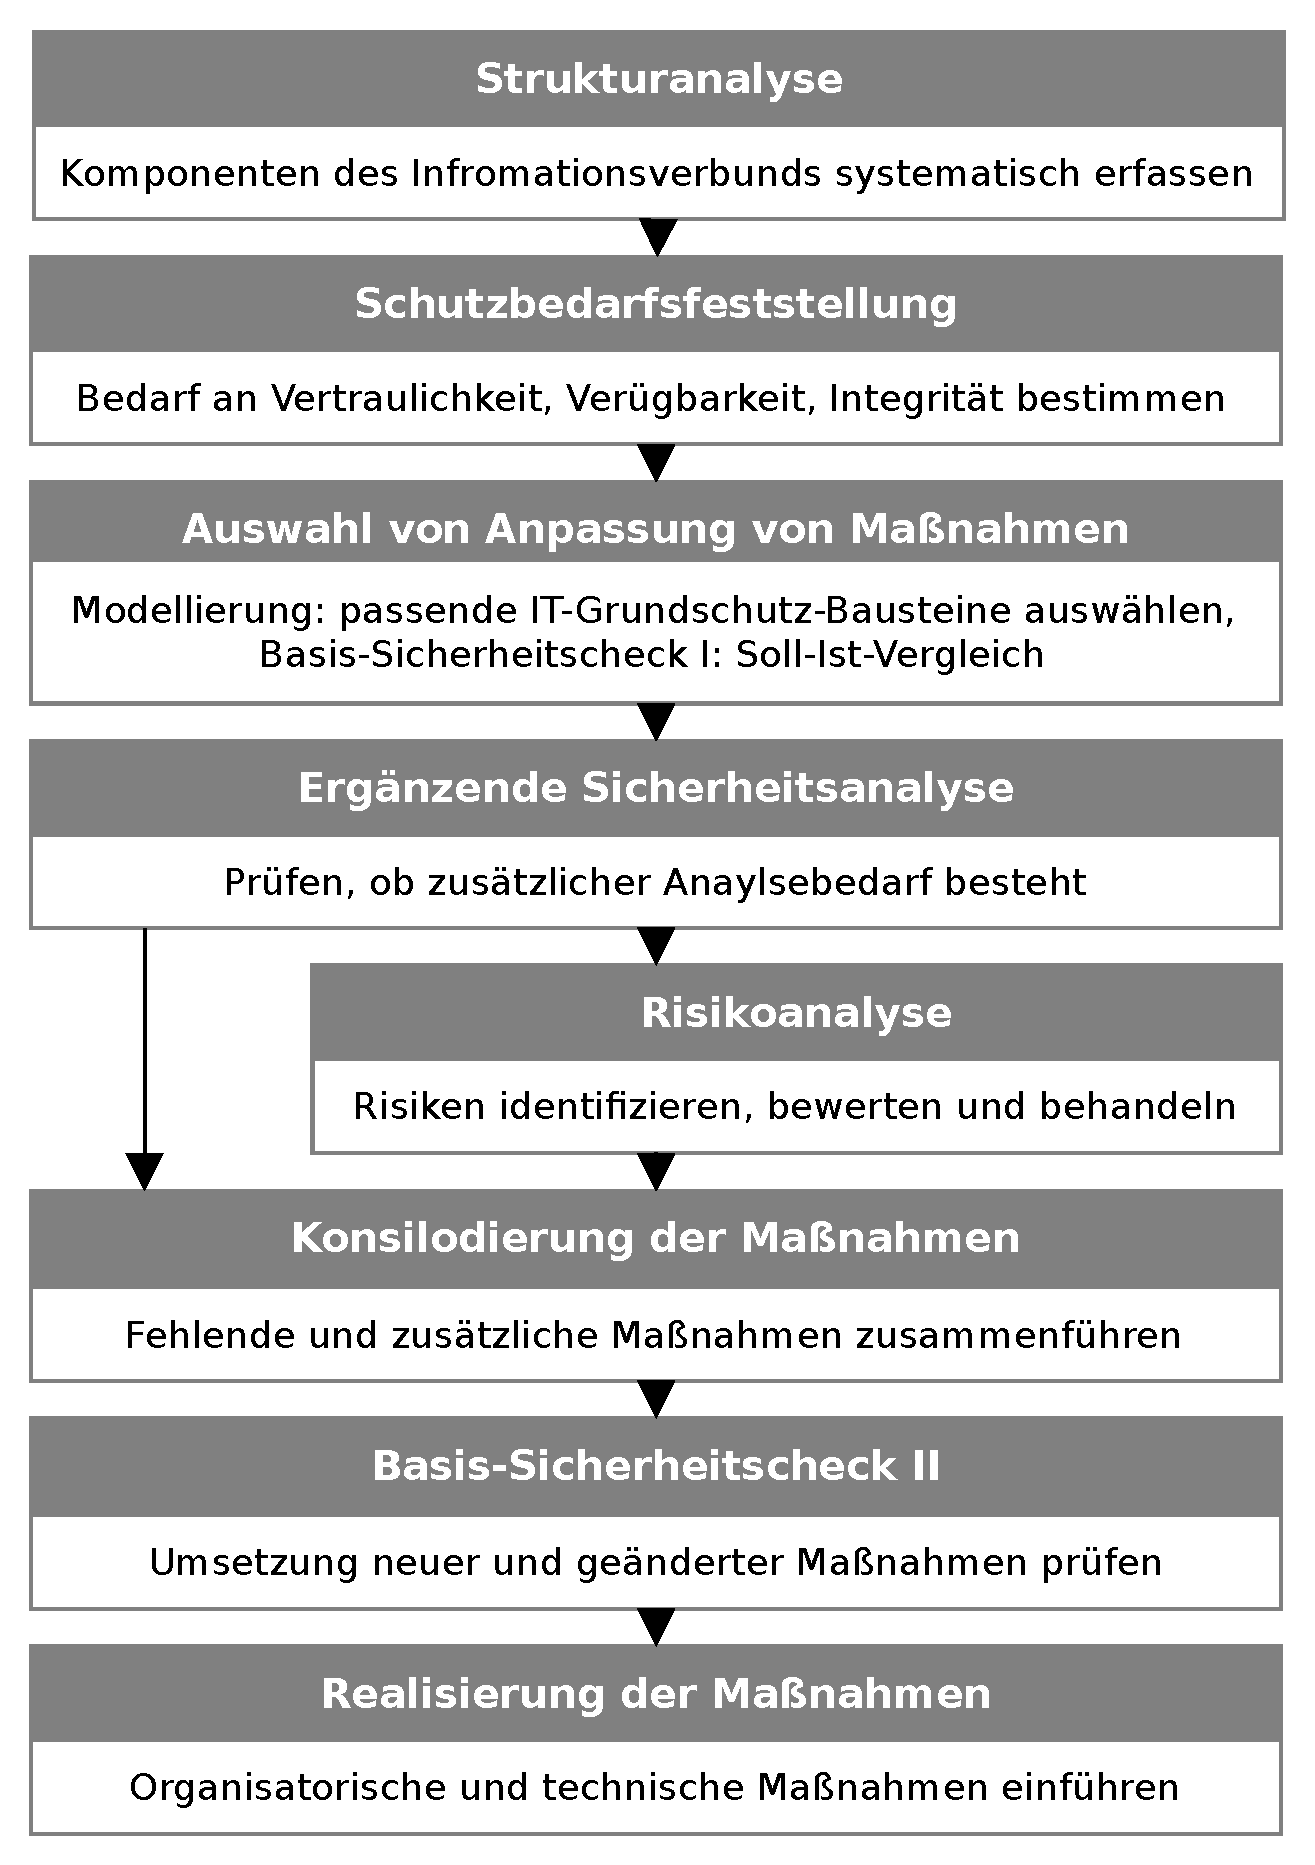
\includegraphics[scale=0.7]{images/bsi_sicherheitskonzept.pdf}
\caption[BSI Sicherheitskonzept]{BSI Sicherheitskonzept\footnotemark}
\label{fig:bsi_sicherheit}
\end{figure}
Ab Schritt sechs erfolgt die Durchführung der Maßnahmen. Bei der Konsolidierung wird geprüft, welche Maßnahmen aus den IT-Grundschutz-Katalogen tatsächlich in der Praxis umsetzbar sind. Teilweise müssen einige Maßnahmen noch an Gegebenheiten im Unternehmen angepasst werden. Unter Berücksichtigung des verfügbaren Budgets und des verfügbaren Personals werden die entsprechenden Maßnahmen für die Umsetzung geplant. Im zweiten Sicherheitscheck wird abschließend ein erneuter Soll-Ist-Vergleich durchgeführt, um die Ergebnisse der Maßnahmen zu überprüfen. Als letzter Schritt werden die Maßnahmen im Alltagsgeschäft in Betrieb genommen.

Das vom BSI vorgeschlagene Konzept und das damit verbundene Vorgehen betrachtet ein Sicherheitsmodell ausgiebig aus technischer Sicht. Es wurde entwickelt, um als internationaler Standard genutzt zu werden, dort hat es jedoch aufgrund schlechter englischer Übersetzungen keinerlei Verbreitung und auch in Deutschland ist die Verbreitung nur sehr gering \cite{bsi_kritik}.

\footnotetext{Der Zeichnung \cite{bsi_img} des BSI nachempfunden, aufgrund unangemessener Bildqualität}

\subsection{Methoden zur Bedrohungsanalyse}

Zusätzlich zum Vorgehen des BSI werden weitere Methoden für die Bedrohungsanalyse vorgestellt, die nützlich für das Erstellen eines Sicherheitskonzepts sind. Denn Aufgrund von Finanznöten des BSI kann sich nicht darauf verlassen werden, dass die Inhalte des IT-Grund\-schutzes immer aktuell sind \cite{bsi_not}.

\subsubsection{Soft Systems Methodology} \label{sec:ssm}

Nachfolgende Erläuterungen beziehen sind auf \cite[s.~252]{gutmann}. 
Das Lösen von Sicherheitsproblemen ist ein kniffeliges Unterfangen, da die typische Vorgehensweise von vielen Informatikern, ein Problem mit Technologien zu bewerfen, nicht funktioniert. Fragt man diese--"Wie löst man das Problem, Benutzer sicher über das Internet zu authentifizieren?"--dann werden Antworten wie OpenID, LDAP, SecurID oder ähnliches zu hören sein. Nur die wenigsten werden fragen--"Wer soll, wo, wogegen authentifiziert werden, wie benutzerfreundlich (einfach) kann der Mechanismus sein und welches Budget steht zur Verfügung?"--Um das natürliche Verlangen, die Lieblingstechnologie verwenden zu wollen, zu unterdrücken, ist es sinnvoll, Problem Structuring Methods (PSK) einzusetzen. Eine dieser PSK-Methoden ist die Soft Systems Methodology (SSM).

\begin{figure}[htbp]
\centering
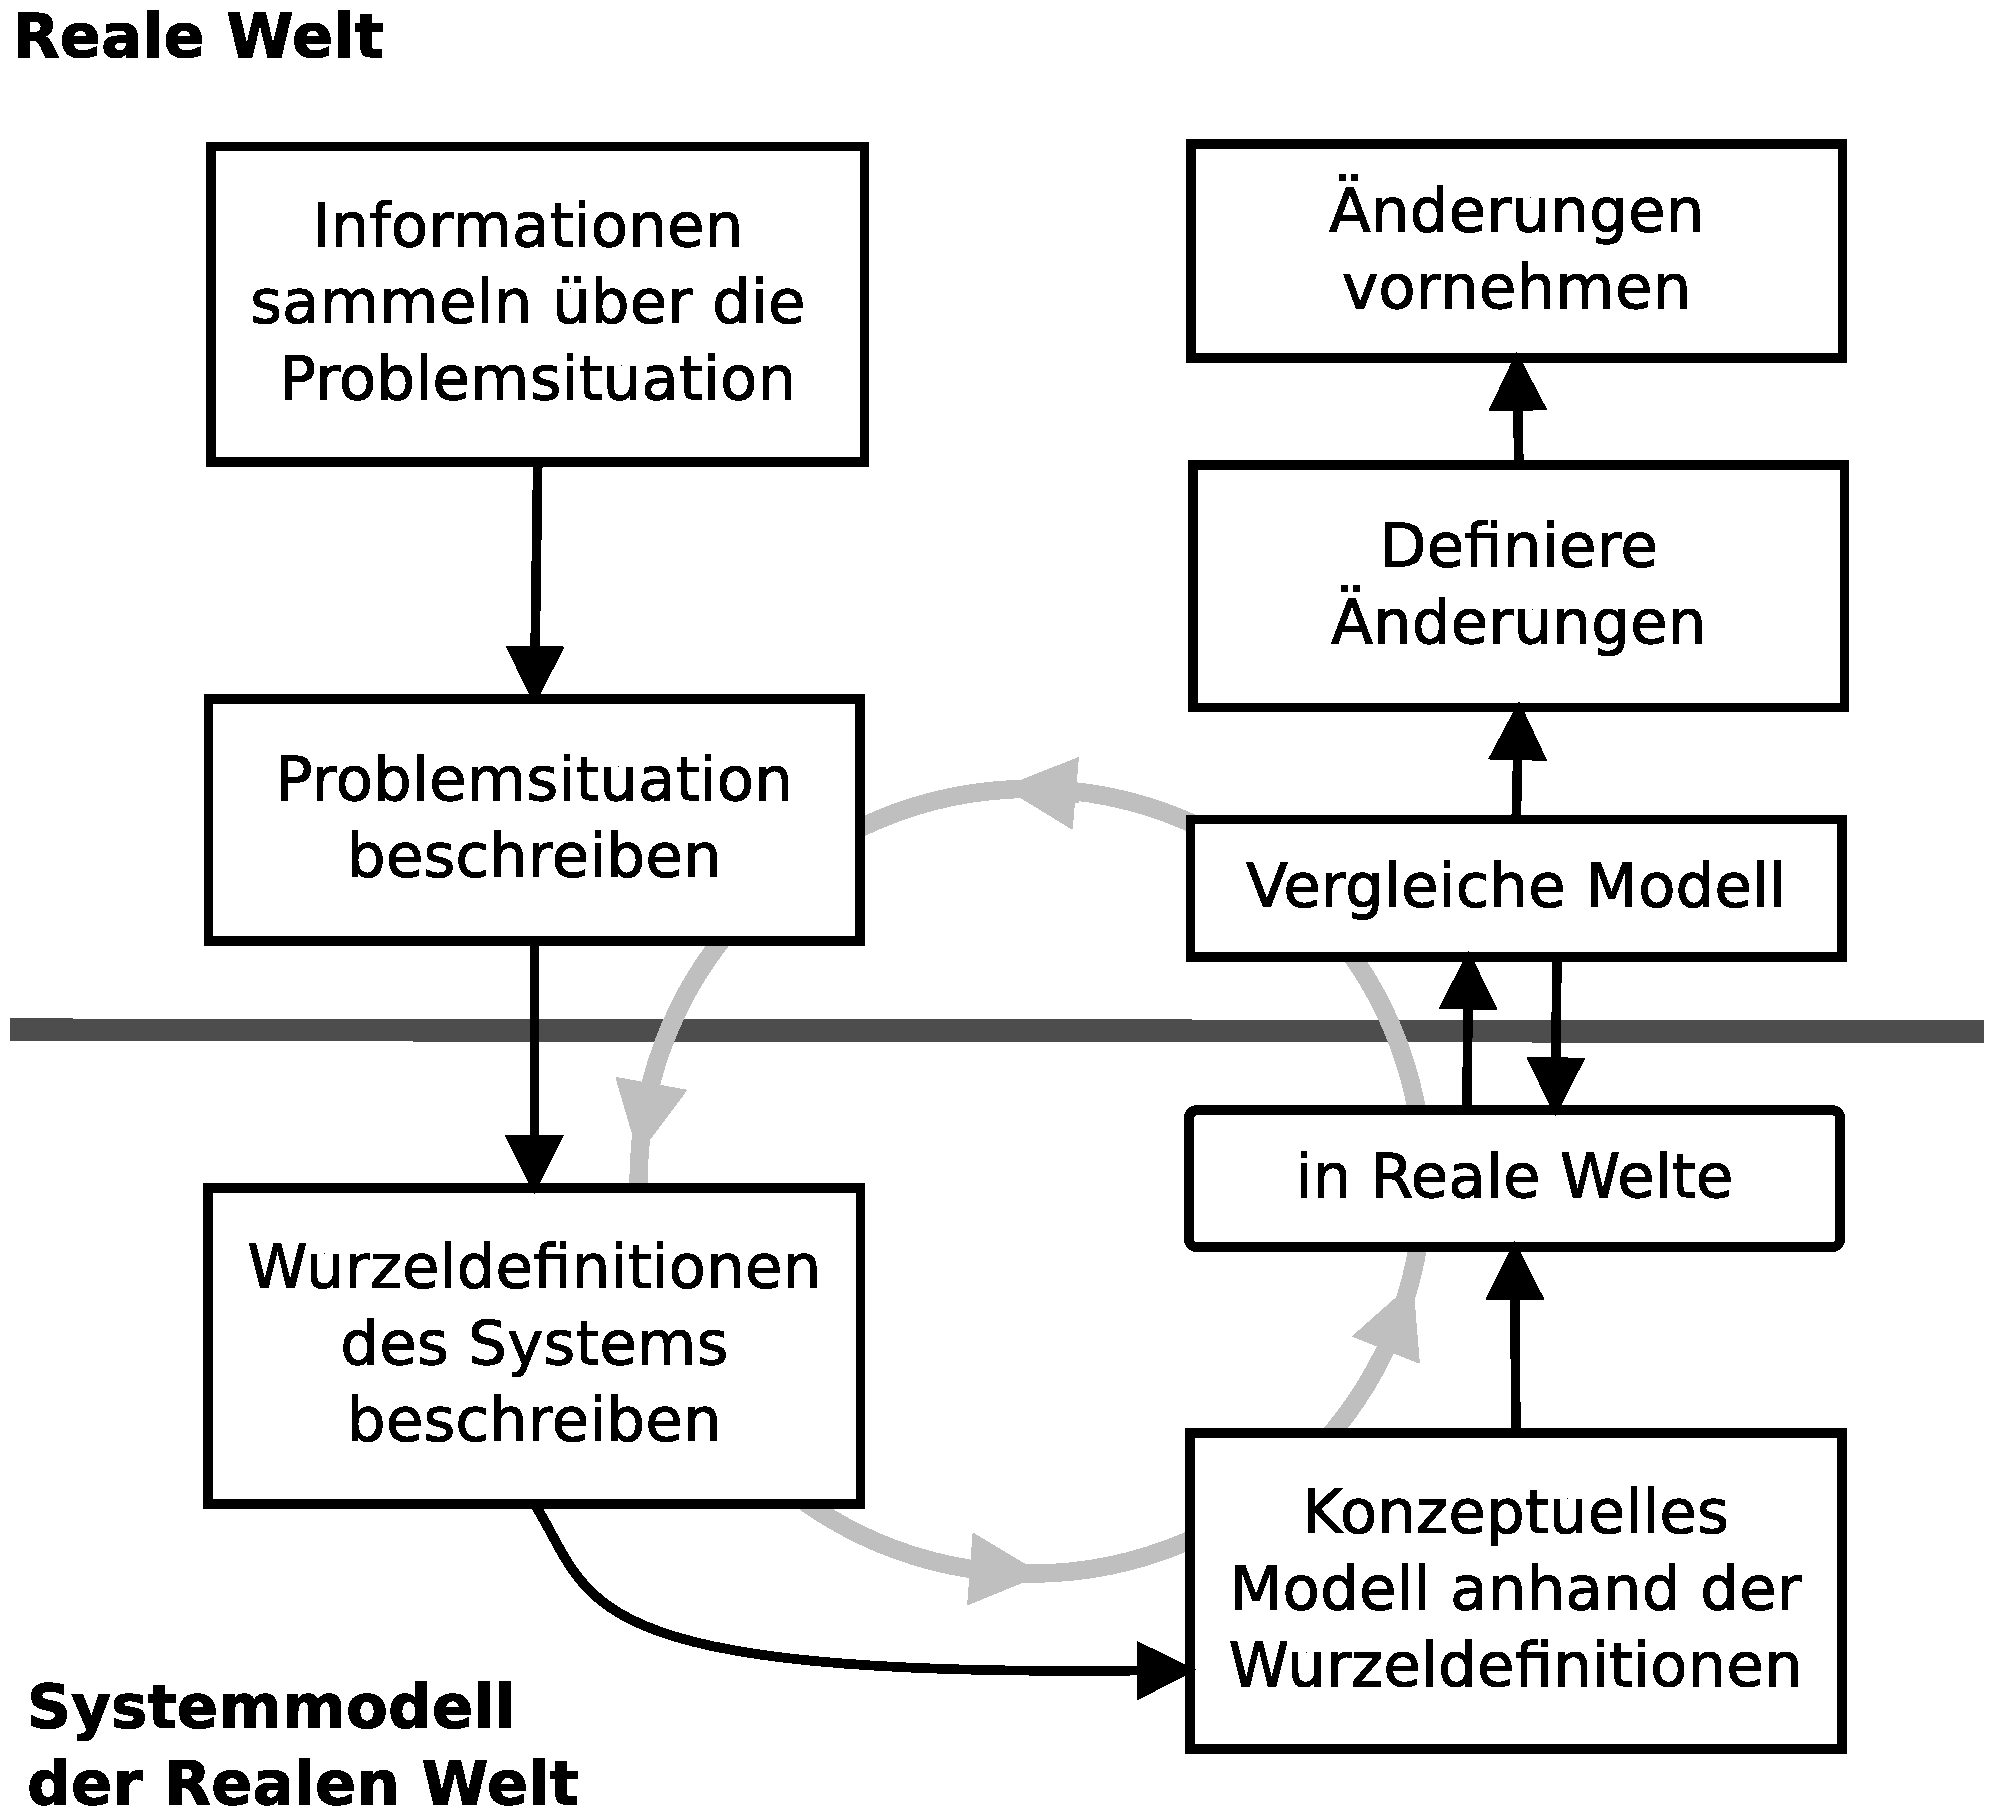
\includegraphics[scale=0.9]{images/ssm.pdf}
\caption{Soft Systems Methodologie}
\label{fig:ssm}
\end{figure}

Die folgenden Inhalte sind den Quellen \cite{checkland, bobwill, ssmger} entnommen. Die Entwicklung von SSM begann in den späten 60er Jahren an der Universität von Lancaster und wurde von Peter Checkland geleitet. Es war zunächst als Modellierungswerkzeug gedacht, wird aber hauptsächlich als Lern- und Bedeutungswerkzeug angesehen, denn SSM kann prinzipiell immer dann eingesetzt werden, wenn jemand versucht, zielgerichtet zu handeln. Das Forscherteam um Peter Checkland hat SSM, beispielsweise während des Flugzeug-Projekts Concorde eingesetzt, bei welchem Sie beauftragt wurden zu helfen. Ein wichtiger Teil von SSM ist die Weltansicht, welche einem Vorgehen Sinn und Zweck verleiht. Beispielsweise ist des einen Terrorist des anderen Freiheitskämpfer. Beide Weltansichten betrachten jedoch dasselbe Geschehen. Durch mehrere zielgerichtete Vorgehen unterschiedlicher Weltansichten wird in SSM versucht, die reale Welt zu beschreiben. Diese ist jedoch viel zu komplex, um in irgendeiner Modellsprache erfasst zu werden. Daher wird das Vorgehen bewusst auf ein rein konzeptionelles Modell beschränkt. Diese Einschränkung verringert die Komplexität und vereinfacht dadurch die Problemlösung. Die Abbildung~\ref{fig:ssm} zeigt die Schritte des SSM-Modells in drei Phasen. Die Trennung zwischen realer Welt und Systemmodell der realen Welt findet zwischen Phasen eins und zwei statt. In der ersten Phase wird die gesamte Problemsituation der realen Welt aus Sicht aller Beteiligten erörtert und unstrukturiert beschrieben. Anhand dieser Informationen wird in der zweiten Phase ein Bild, in SSM-Terminologie Rich-Picture genannt, erstellt. Dieses ist ein wichtiges Hilfsmittel zur Beschreibung der Problemsituation, welches möglichst viele Informationen in einem Bild erfassen soll. Mit dessen Hilfe sollen Grenzen, Struktur, Informationsflüsse, Kommunikationskanäle und das menschliche Aktivitätssystem eines Systems aufzeigt werden. Das Bild dient als Grundlage für die Ursachendefinitionen, welche einen festen Rahmen für die konzeptionellen Modelle ermöglichen. Die Ursachendefinitionen sorgen dafür, dass wichtige Aspekte nicht weggelassen werden. Die Gedächtnisstütze CATWOE\footnote{Übersetzungen wurden aus dem Artikel \cite{ssmger} übernommen.} ist eine Empfehlung zur Erstellung der Ursachendefinitionen:

\begin{itemize}[leftmargin=*]
\item \textbf{Client (Kunde)}, wer oder Was profitiert von dem Umwandlungsprozess.
\item \textbf{Actor (Akteur)}, wer ermöglicht den Kunden den Umwandlungsprozess.
\item \textbf{Transformation process (Umwandlungsprozess)}, von einem Startzustand in eine Endzustand.
\item \textbf{Weltanschauung}, gibt dem Umwandlungsprozess Bedeutung.
\item \textbf{Owner (Inhaber)}, vor wem muss sich das System verantworten und/oder wer kann veranlassen, dass es nicht existiert.
\item \textbf{Environmental constraints (Randbedingungen)}, was beeinflusst das System, ohne es zu kontrollieren.
\end{itemize}

Die Rollen welche Kunde, Akteur und Inhaber belegen, können in bestimmten Fällen überlappen. CATWOE ist keine willkürlich Ansammlung von Eigenschaften, sondern resultiert aus Beobachtungen der realen Welt. Bei der Ausübung von SSM ist aufgefallen, dass insbesondere Akteur und Inhaber oft bei der Betrachtung ausgelassen werden, da diese "zu offensichtlich" erscheinen \cite[s.~255]{gutmann}. Die Reihenfolge, in welcher die Eigenschaften abgearbeitet werden, ist beliebig. Je nach Problemsituation sind einige Eigenschaften offensichtlicher als andere. Die konzeptionellen Modelle, welche aus den Ursachendefinitionen gebildet wurden, dienen dazu, Debatten über die Thematik zu strukturieren, indem sie mit der realen Welt verglichen werden. In einem iterativen Prozess werden die ersten beiden Phasen wiederholt, bis die Thematik klar genug ist, um Ergebnisse zu treffen. Die Ergebnisse werden abschließend, in Phase drei, in konkrete Schritte formuliert, die ausgeführt werden sollen.

Die Soft Systems Methodology ist zwar keine Methodik, die explizit zur Erstellung eines Sicherheitskonzeptes gedacht ist, ihre Vorgehensweise für die Analyse, durch Trennung von realer Welt und deren Abstraktion, jedoch gut geeignet zum Lösen beliebiger Problemstellungen. SSM nimmt bewusst Einfluss auf das menschliche Denken und Vorgehen, um dieses zu fokussieren und dadurch zu optimieren.

\subsubsection{Data Flow Diagramme}

Der nachfolgender Paragraph bezieht sich auf \cite[s.~263]{gutmann}.
Durch die Bedrohungsanalyse (Kapitel~\ref{chap:threat_analysis}) mittels SSM wird geklärt, gegen welche Bedrohungen geschützt werden soll und welche Maßnahmen dafür notwendig sind. Darauf aufbauend kann die Bedrohungsmodellierung der Implementierung, unter Verwendung von Data Flow Diagrammen, angewandt werden. Data Flow Diagramme (DFD) gehen zurück auf die 70er Jahre. Ihre Aufgabe ist es, die gefährdeten Informationen der Applikation zu identifiziert, die Bedrohungen zu finden und Maßnahmen dagegen zu treffen. Es gibt mehrere Level von DFDs, welche den Detailgrad des Diagramms bestimmen. Für die Bedrohungsmodellierung reicht Level 0 aus. Es zeigt den Informationsfluss zwischen internen und externen Anwendungsgrenzen. Für die Bedrohungsmodellierung wird der Aufbau der Diagramme auf die fünf Objekte (Abbildung~\ref{fig:dfd_intro}) beschränkt. Die Vertrauensgrenze ist ein Objekt, dass das klassische DFD erweitert, um den Aspekt der Bedrohungen eines System darstellen zu können. Generell gilt, überschreitet eine Datenfluss eine Vertrauensgrenze, ist er durch Bedrohungen verwundbar.

\begin{figure}[htbp]
\centering
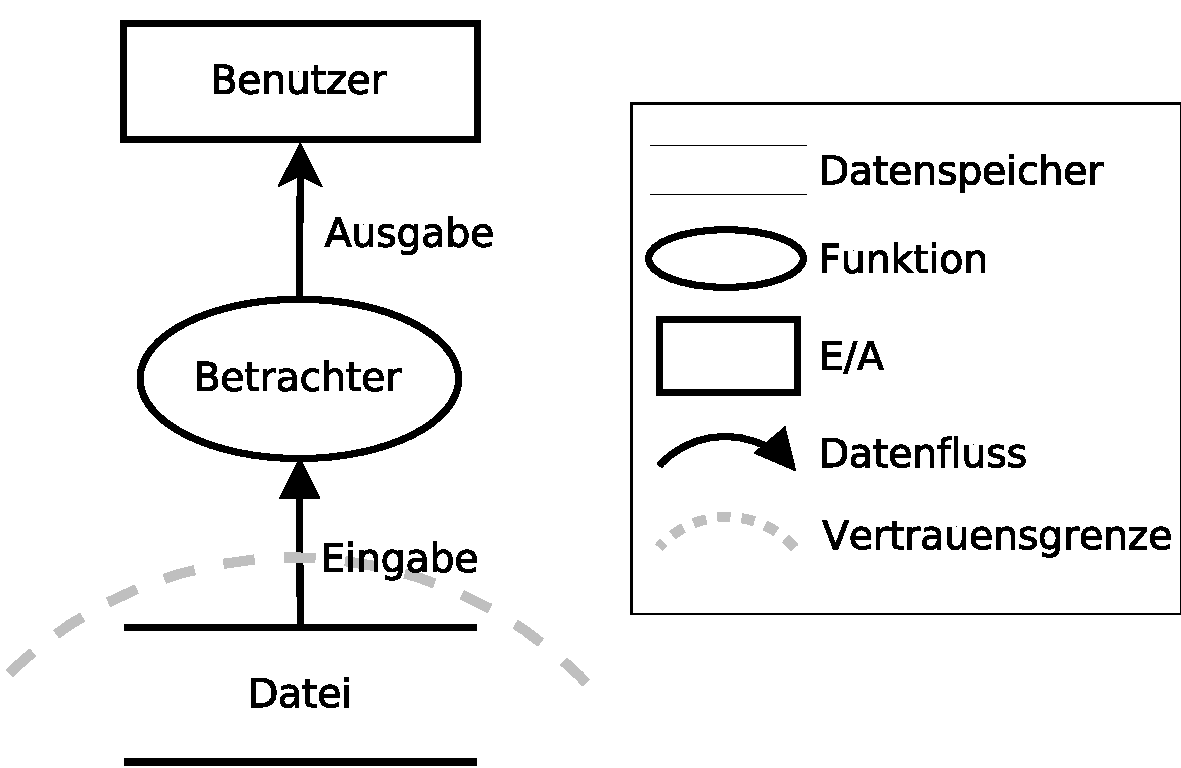
\includegraphics[scale=0.4]{images/dfd_intro.pdf}
\caption{Data Flow Diagramm Beispiel}
\label{fig:dfd_intro}
\end{figure}

Anhand der Data Flow Diagramme werden Gefährdungen für Informationsflüsse gesucht. Diese werden zunächst einfachheitshalber in fünf Kategorien gegliedert werden:

\begin{table}[h] % htbp ~ here, top, bottom, page
\begin{tabularx}{\linewidth}{@{}lX@{}}
\textbf{Sabotage} & unentdeckt Daten modifizieren\\
\textbf{Personifikation} & vorgeben, jemand oder etwas Anderes zu sein\\
\textbf{Informationspreisgabe} & unberechtigter Zugriff auf Informationen\\
\textbf{Disput} & meiden der Verantwortung für ein Tun oder Nichttun\\
\textbf{Denial of Service} & einen Service an seiner Ausführung hindern\\
\end{tabularx}
\end{table}

Denial of Service (DoS) ist eine sehr allgemeine Gefährdung, deshalb soll diese nur bei Netzwerkzugriffen berücksichtigt werden. Auf Grundlage dieser fünf Kategorien können detaillierte Analysen durchgeführt werden.

\section{Authentifizierungsverfahren} \label{sec:auth_modells}

Für die Authentifizierung gibt es verschiedene Möglichkeiten, diese unterscheiden sich sowohl in ihrem Aufwand als auch ihrem Nutzen. Zuvor wird noch der Begriff "Vertrauen" definiert.

\subsection{Vertrauen}

Vertrauen ist der Zustand, der durch Authentifizierung erreicht werden soll. Vertrauen sagt aus, dass ein Partner einem anderen Partner in Funktion, Ehrlichkeit und Zuverlässigkeit, aufgrund von eigenen Erfahrungen, glaubt \cite{chen}. Dabei unterscheidet man einseitiges und beidseitiges Vertrauen. Von einseitigem Vertrauen wird gesprochen, wenn nur ein Partner einen Nachweis seiner Identität erbracht hat. Bei beidseitigem Vertrauen haben beide Kommunikationspartner gegenseitig überprüft, dass der Andere derjenige ist, welcher er vorgibt zu sein.

\subsection{Passwörter}

Bei passwortbasierter Authentifizierung weist sich ein Kommunikationspartner über einen eindeutigen Namen und ein Passwort gegenüber einem anderen Kommunikationspartner aus. Passwortbasierende-Authentifizierung wird meistens verwendet, um einseitiges Vertrauen herzustellen. Der typische Einsatz ist die Anmeldung an einem Server, um Zugriff auf dessen Services zu erhalten. Der Benutzer weist sich mit Name und Passwort gegenüber dem Server aus, umgekehrt gibt es oft keinen Nachweis über die Identität. Eine Möglichkeit des Identitätsnachweises von Serverseite sind Zertifikate (vgl.~\ref{sec:auth_asym}). Die Sicherheit von Passwörtern basiert auf der Annahme, dass der Benutzer ein sicheres Passwort gewählt hat und dieses stets vor fremden Zugriff schützt. Die Realität zeigt jedoch, dass diese Annahme selten zutrifft \cite[s.~2]{gutmann}.

\subsection{Symmetrisch}

Symmetrische Verfahren arbeiten mit einem Passwort oder Schlüssel, der beiden Kommunikationspartnern bekannt ist. Dieser muss vor der Kommunikation, über einen zweiten Kanal, etwa persönlich, ausgetauscht werden. Das Verfahren wird deshalb auch als Pre-Shared-Key (PSK) bezeichnet. Die verbreitetste Anwendung von PSKs sind WLAN-Netzwerk im privaten Bereich. Zugang zu einem solchen WLAN-Netzwerk kann jeder erhalten, der den Schlüssel kennt. Unter der Annahme, dass nur Berechtigte den Schlüssel kennen, wird ein Vertrauensverhältnis zwischen den Kommunikationspartnern in dem Netzwerk aufgebaut. Bei steigender Anzahl der Kommunikationspartner wird dieses System unbrauchbar, denn jeder neue Partner erhält den gleichen Schlüssel. Soll nun einem Berechtigten der Zugriff verboten werden, muss der Schlüssel gewechselt werden. Dies führt dazu, dass alle, außer demjenigen, dem die Berechtigung entzogen werden soll, einen neuen Schlüssel benötigen.

\subsection{Asymmetrisch} \label{sec:auth_asym}

Asymmetrische Verfahren arbeiten mit zwei Schlüsseln, einem öffentlichen und einem privaten (Abbildung~\ref{fig:pp_keygen}). Der öffentliche Schlüssel wird dem Kommunikationspartner übergebenen, der private Schlüssel bleibt im eigenen Besitz und wird vor fremden Zugriff geschützt. 

\begin{figure}[htbp]
\centering
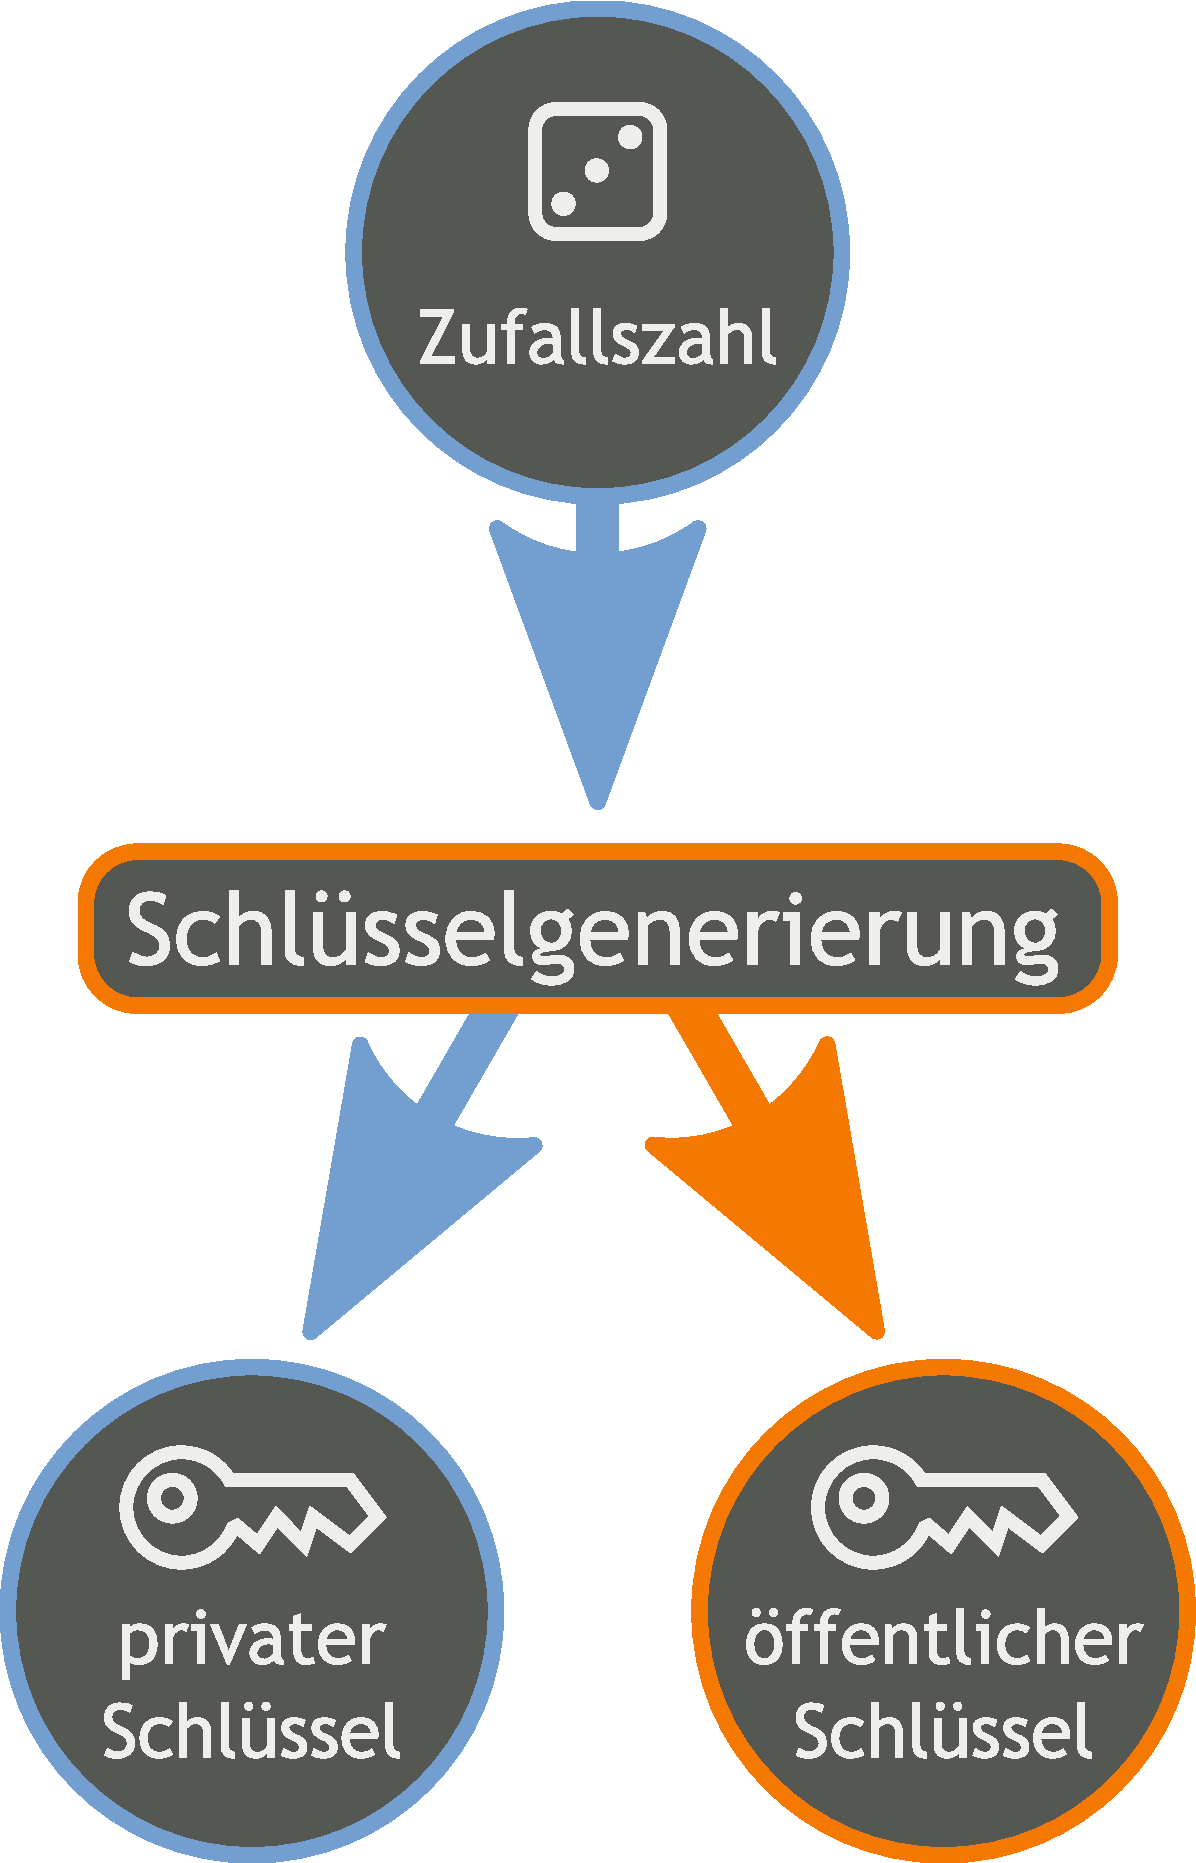
\includegraphics[scale=0.2]{images/public_private_keygeneration.pdf}
\caption{Public/Private Schlüsselgenerierung aus \cite{wiki_asym_crypto}}
\label{fig:pp_keygen}
\end{figure}

Der große Vorteil dieses Verfahrens gegenüber den Symmetrischen ist, das der öffentliche Schlüssel über einen nicht vertrauenswürdigen Kanal geteilt werden kann. Bei der Authentifizierung wird der private Schlüssel genutzt, um eine Nachricht zu signieren. Mit dem öffentlichen Schlüssel kann der Kommunikationspartner verifizieren, dass die Nachricht von dem Kommunikationspartner kommt, der den passenden privaten Schlüssel hat (Abbildung~\ref{fig:pp_veri}). Dadurch kann festgestellt werden, ob die Nachricht auf dem Transportweg manipuliert worden ist, allerdings bleibt das Problem des Vertrauens, denn ob der Schlüssel von demjenigen stammt, der der Kommunikationspartner vorgibt zu sein, ist dadurch nicht garantiert. Hierbei wurde die Notwendigkeit nach einem expliziten Austauschkanal eliminiert, da der Schlüsselaustausch, über einen unsicheren Kanal erfolgen kann. Allerdings hat man dadurch das Bedürfnis nach einen Authentifizierungskanal geschaffen, um eine Identitätsprüfung durchführen zu können.
 
\begin{figure}[htbp]
\centering
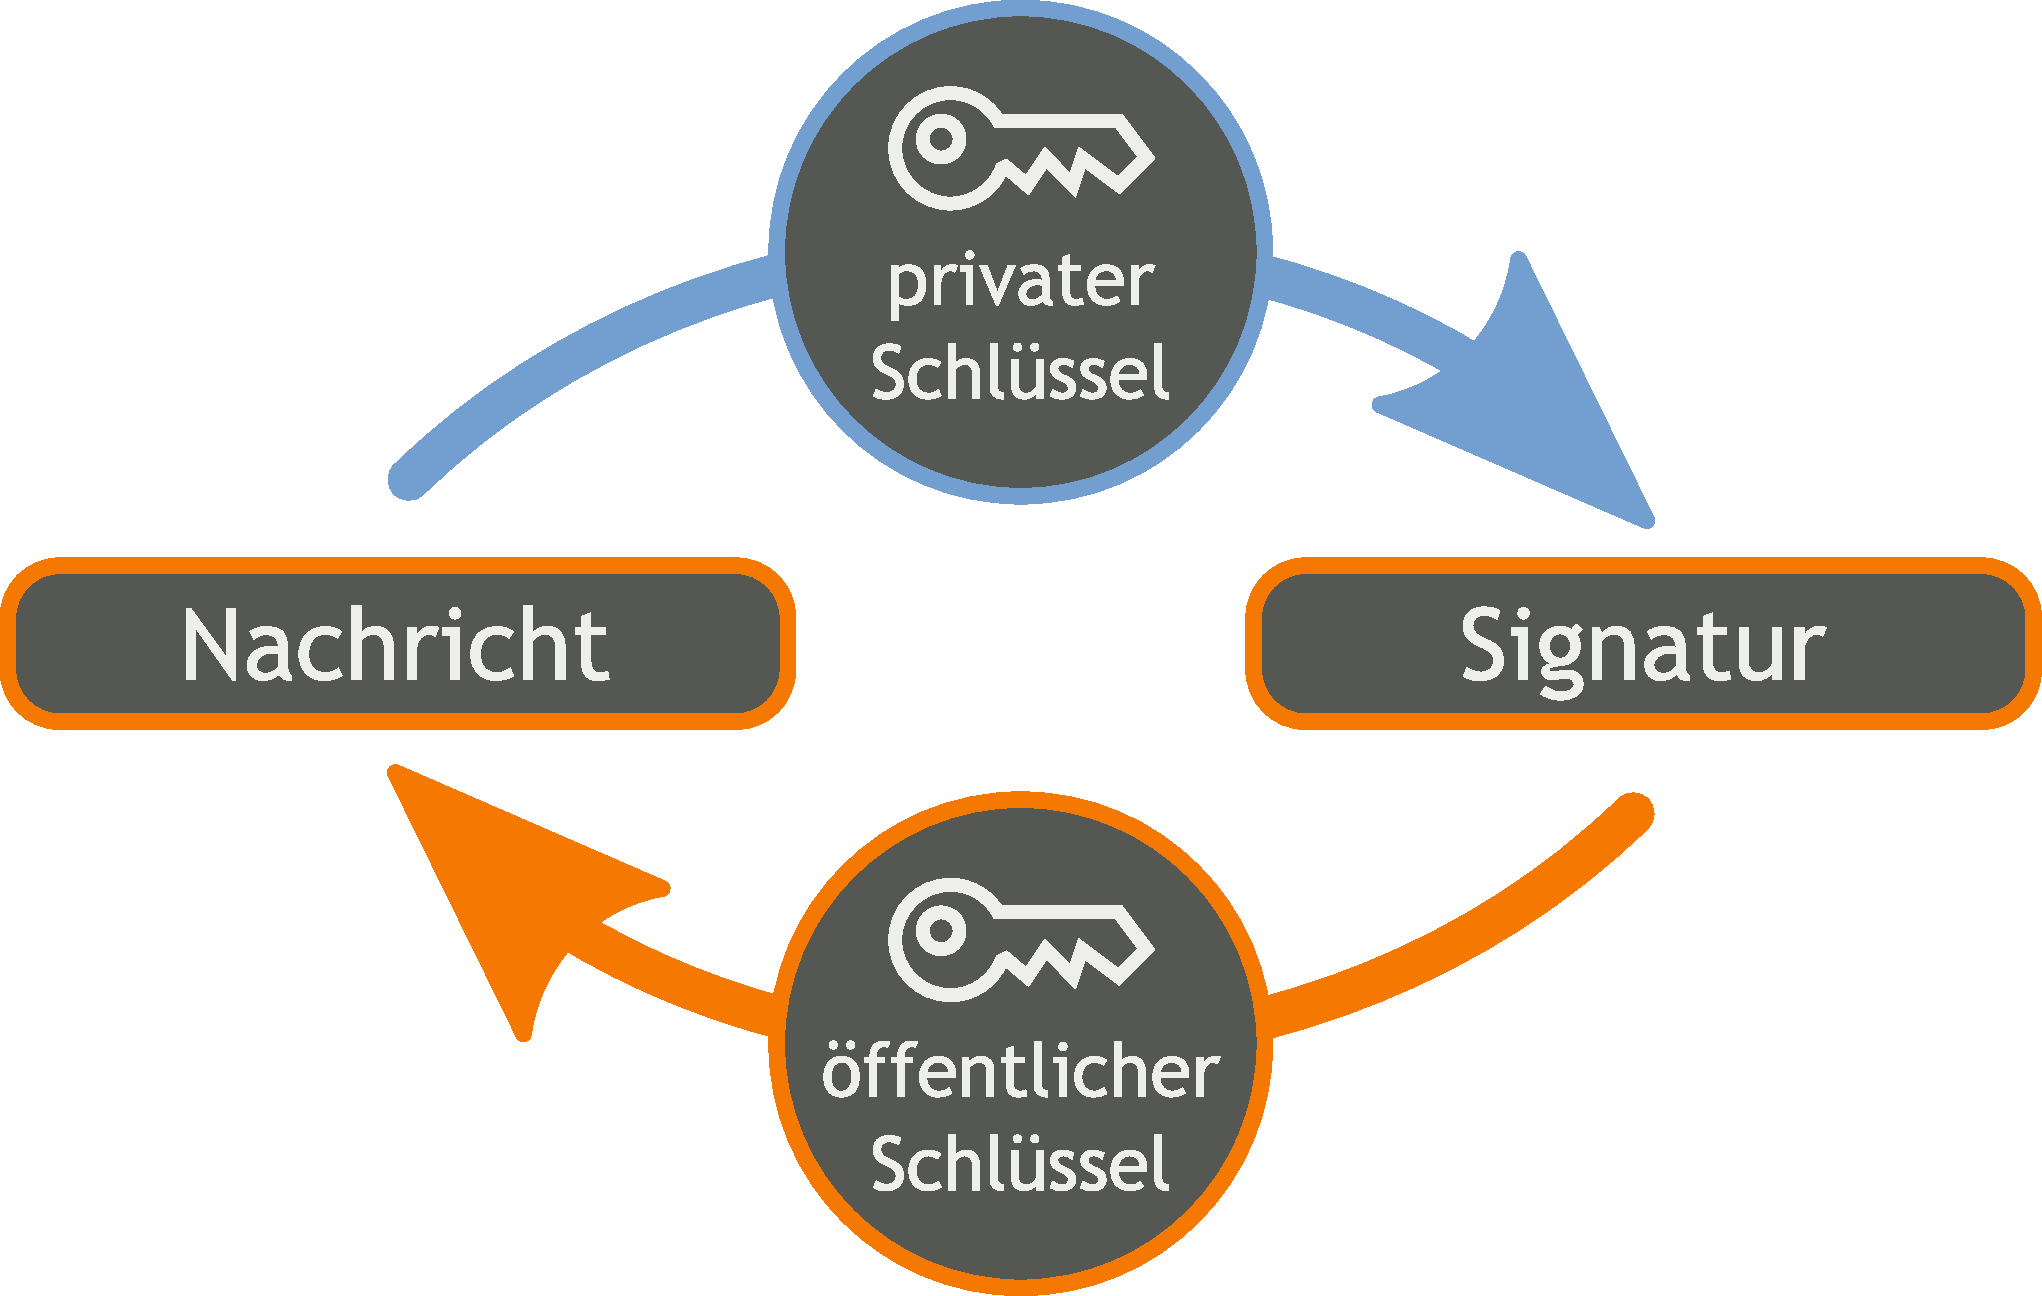
\includegraphics[scale=0.2]{images/public_private_verification.pdf}
\caption{Public/Private Verifizierung aus \cite{wiki_asym_crypto}}
\label{fig:pp_veri}
\end{figure}

Aus diesem Hintergrund wurden Zertifikate erschaffen. Der heutige verbreitetste Standard sind Zertifikate im X.509-Format. Ein Zertifikat beinhaltet Informationen über den Inhaber, die Zertifizierungsstelle, die Gültigkeit und den öffentlichen Schlüssel. Anstatt den öffentlichen Schlüssel auszutauschen, wird nun das Zertifikat gesendet. Bei der Zertifizierungsstelle kann die Echtheit verifiziert werden. 

\chapter{Bedrohunganalyse} \label{chap:threat_analysis}
\epigraphhead[70]{\epigraph{The only truly secure system is one that is powered off, cast in a block of concrete and sealed in a lead-lined room with armed guards.}{\textit{Gene Spafford}}}

Als erstes wird in diesem Kapitel die Zielsetzung dieser Thesis beschrieben. Die eigentliche Bedrohungsanalyse gliedert sich in die drei SSM-Phasen, die in Abschnitt~\ref{sec:ssm} beschrieben sind. Zunächst wird die Problemsituation beschrieben, danach werden zwei konzeptionelle Modelle aus unterschiedlichen Weltansichten erstellt. Die unterschiedlichen Weltansichten entstammen der Betrachtung eines Beschützers und eines Angreifers des Systems. Durch den Vergleich der konzeptionellen Modelle mit der realen Welt werden konkrete Maßnahmen formuliert. Das Ergebnis der Bedrohungsanalyse soll mögliche Bedrohungen aufdecken und erste Maßnahmen hervorbringen. 

\section{Zielsetzung}

Ziel dieser Thesis ist es, einen Lösungsvorschlag zur Authentifizierung und Autorisierung für den Fernzugriff auf den Marktrechner zu unterbreiten. Abbildung~\ref{fig:uc_solution} zeigt die dafür relevanten Use-Cases. Auf der linken Seite sind die Benutzer zu sehen. Diese wollen lokal oder remote bestimmte Funktionen auf dem Marktrechner aufrufen. Dazu müssen Sie vorher authentifiziert und autorisiert werden. Die Autorisierung soll auf einem Rollenmodell basieren, wobei ein Benutzer mehrere Rollen innehaben kann. Die Benutzung über den Remotezugriff soll über HTTPS und das RestGateway des Marktrechners erfolgen. Zur Überprüfung der Authentifizierungs- und Autorisierungsdaten des Nutzers soll ein Authentifizierungs- und  Autorisierungs-Server (AAS) kontaktiert werden. Dieser AAS kann räumlich getrennt von den Benutzern, etwa über das Internet, erreichbar sein. Der Marktrechner soll die Möglichkeit bieten, mehrere AAS abfragen zu können.

\begin{figure}[htbp]
\centering
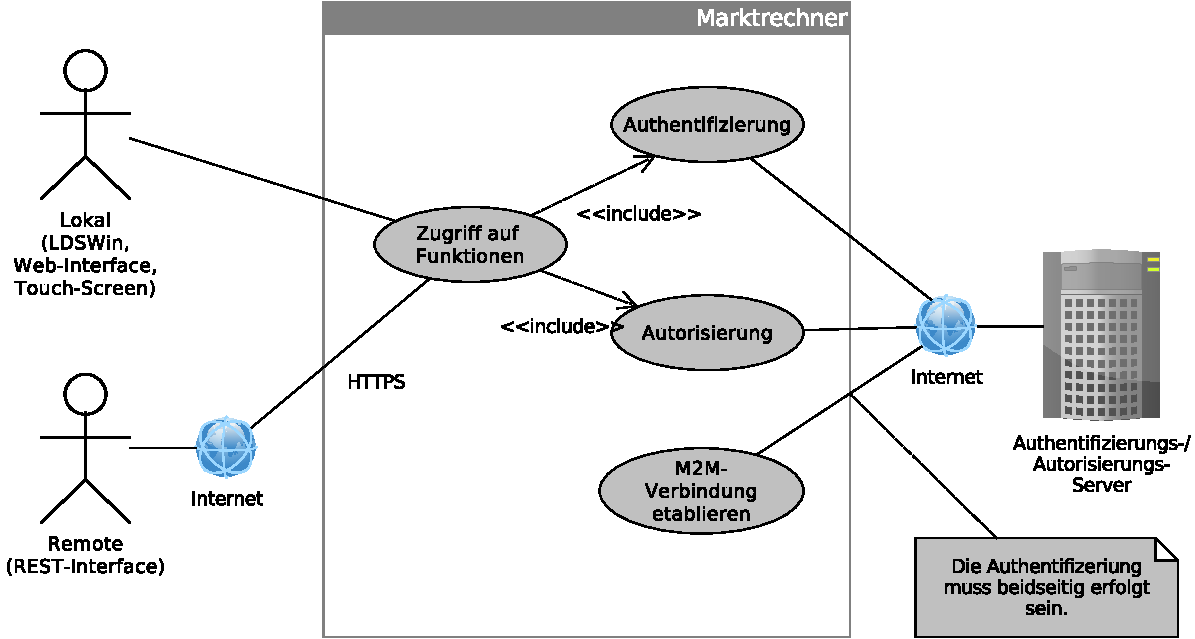
\includegraphics[scale=0.6]{images/ziel_usecase.pdf}
\caption{Zielsetzung Use-Case-Diagramm}
\label{fig:uc_solution}
\end{figure}

\subsection{Vorgehen}

Im Grundlagenteil~\ref{sec:sec_standard} wurde die Common Criteria als internationaler Sicherheitsstandard vorgestellt, welcher für die Entwicklung sicherer Systeme verwendet wird. Das für diese Thesis relevante Protection Profile analysiert die aus Kundensicht relevanten Anforderungen des zu sichernden Systems. Ein komplettes PP zu erstellen, würde den Rahmen der Thesis sprengen, deswegen werden die wichtigsten Aspekte herausgenommen und behandelt. Dazu werden zunächst die zu schützenden Güter und deren Bedrohungen analysiert. Anschließend werden Maßnahmen zu den Bedrohungen gesucht. Dabei soll zunächst vermieden werden, Bezug auf eine bestimmte Technologie oder ein bestimmtes Konzepte zu nehmen, außer die Randbedingungen beziehungsweise Maßnahmen lassen keine alternativen Lösungen zu. Zum Schluss werden die Kriterien aufgestellt, anhand welcher die Evaluierung durchgeführt werden soll.

\subsection{Methoden}

Als Methoden für die Erkennung der Bedrohungen werden die Soft Systems Methodology und Data Flow Diagramme eingesetzt. Unterstützend werden Gefährdungenkataloge und Maßnahmenkataloge aus dem IT-Grundschutz des BSI herangezogen. 

Der BSI hat Gefährdungen und Maßnahmen zu Bausteinen zusammengefasst, die sich in fünf Kategorien gliedern:

\begin{itemize}
\item Übergreifende Aspekte
\item Infrastruktur 
\item IT-Systeme
\item Netze 
\item Anwendungen
\end{itemize} 

Die Übergreifenden Aspekte beinhalten wichtige Bausteine, etwa Datensicherungskonzept, Sensibilisierung und Schulung zur Informationssicherheit oder Behandlung von Sicherheitsvorfällen. Mit dem Blick auf den Schwerpunkt dieser Thesis, wird aus dieser Kategorie lediglich auf das Kryptokonzept eingegangen. Aus dem selben Grund werden die Bausteine aus der Kategorie Infrastruktur nicht weiter betrachtet. Ebenso werden die Gefährdungen der höheren Gewalt und die Maßnahmen der Notfallvorsorge nicht betrachtet.

Die Bedrohungsanalyse bewegt sich auf einem abstrakten generischen Level, weshalb die Kategorien IT-Systeme und Netze hier nicht betrachtet werden. In der anschließenden Bedrohungsmodellierung wird das System konkretisiert, womit diese Bausteine dann zur Geltung kommen. Jeder Abschnitt in diesen beiden Kapiteln erklärt seine relevanten Bausteine, Gefährdungen und Maßnahmen.

\section{Beschreibung der Problemsituation} \label{sec:problem_situation}

Die in Abschnitt~\ref{sec:marktrechner} geschilderte Architektur des Marktrechnerumfeldes wird mit dem Rich-Picture in Abbildung~\ref{fig:problem_situation} auf Sicherheitsmängel untersucht. Der Fokus dieser Arbeit liegt auf dem Fernzugriff, dennoch werden auch die Probleme des lokalen Zugriffes erfasst. Dadurch soll verhindert werden, dass der Fernzugriff unnötige Hindernisse für die lokale Zugriffskontrolle schafft. 

\begin{figure}[htb]
\centering
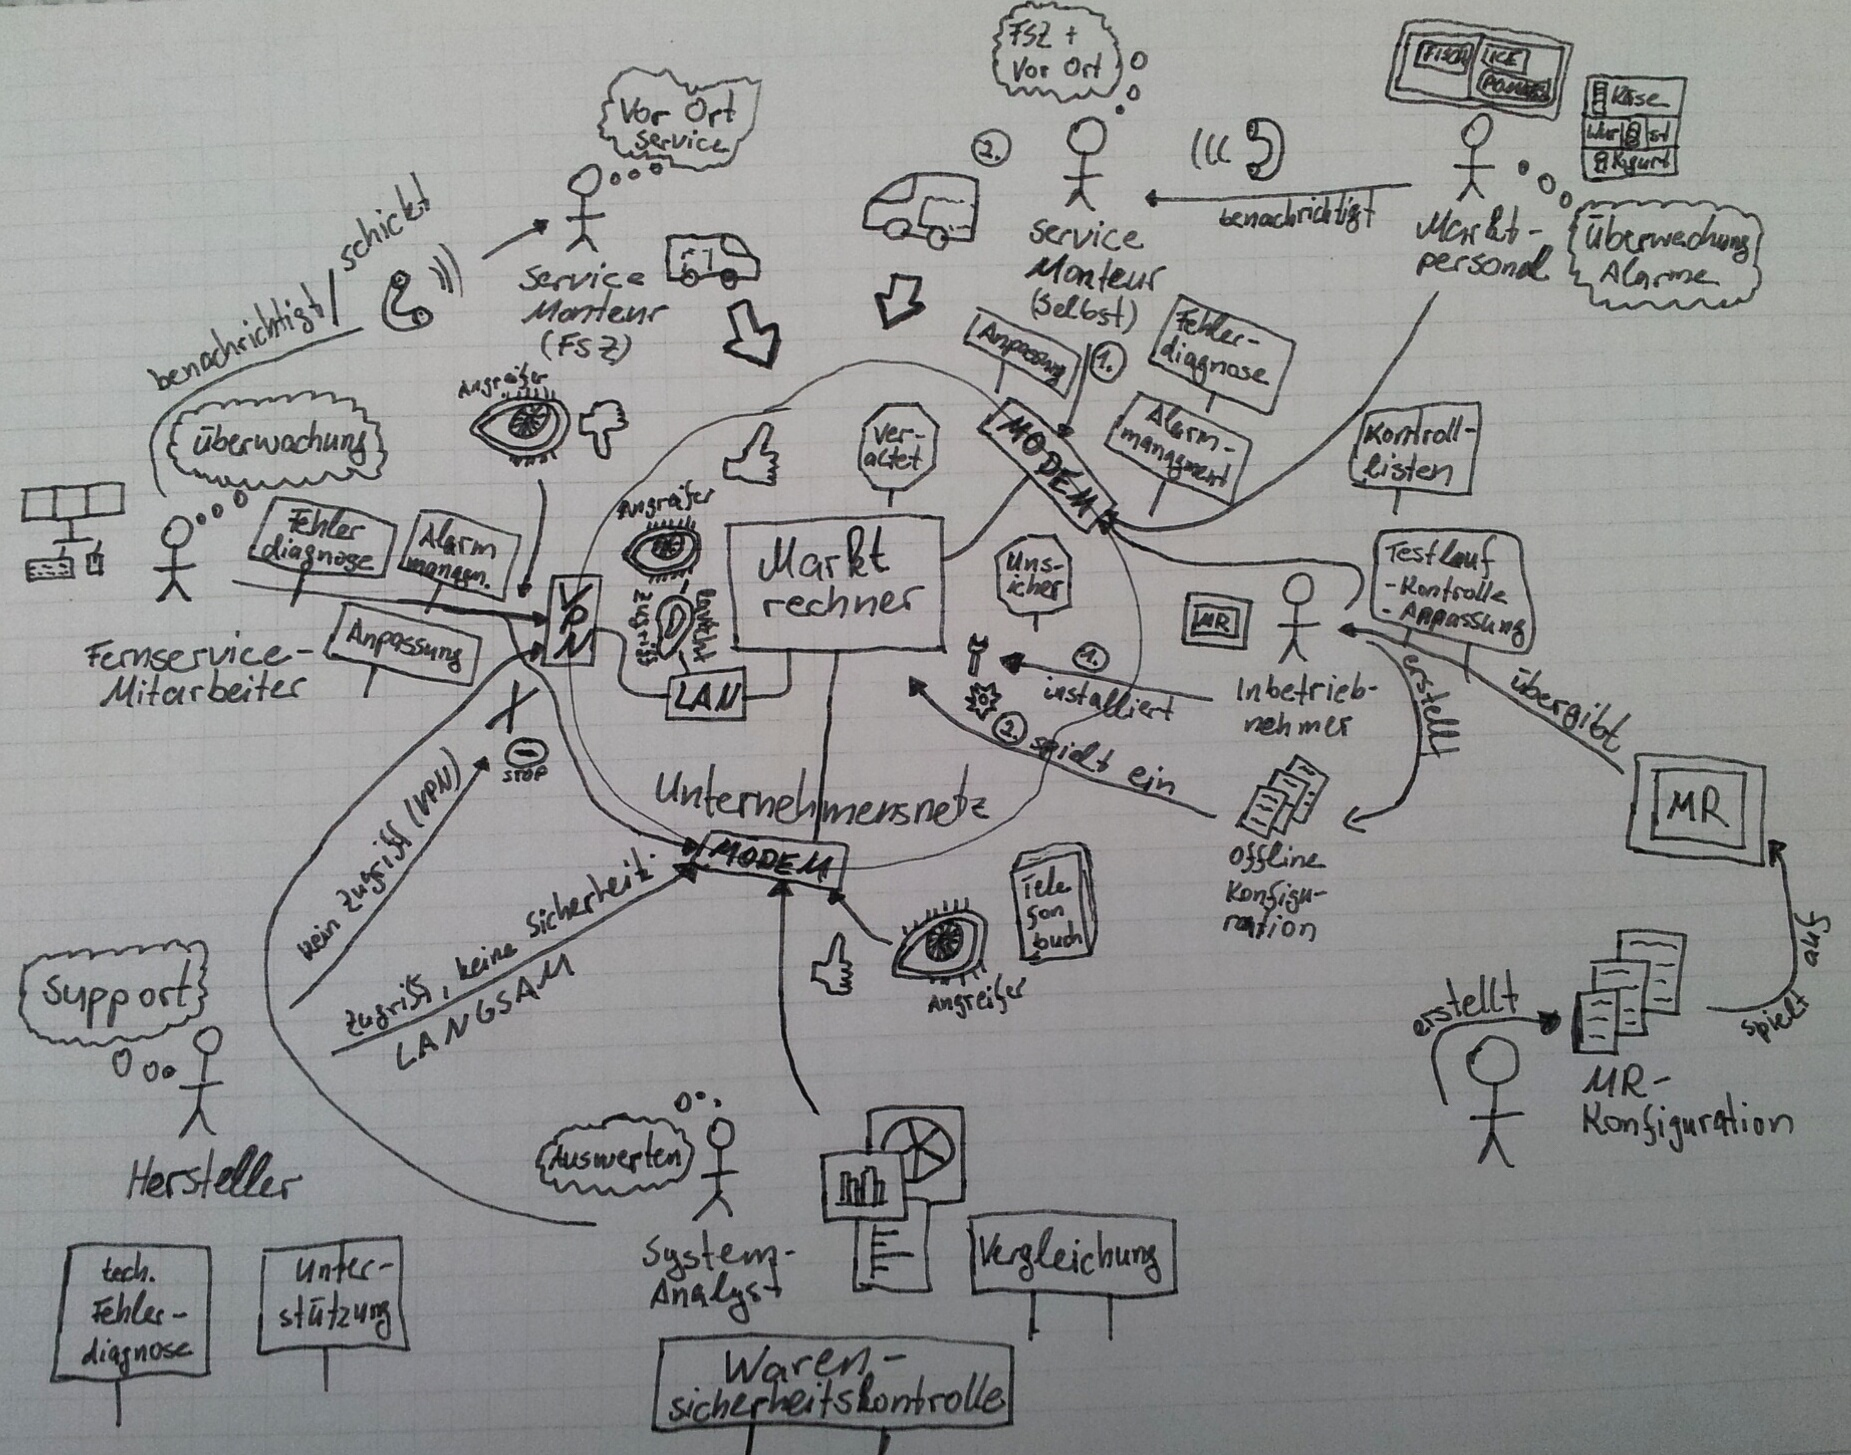
\includegraphics[scale=0.215]{images/problemsituation.jpg}
\caption{Problemsituation}
\label{fig:problem_situation}
\end{figure}

\subsection{Identifizieren der Rollen} \label{sec:roles}

Zunächst wird ein Überblick über alle Zugriffsberechtigten geschaffen. Diese werden anhand von Rollen zusammengefasst, welche Funktion und Zugriffsart beschreiben. Alle Rollen sind in der Abbildung~\ref{fig:problem_situation} illustriert. Die Beschreibungen der Rollen sind allgemein gehalten und nehmen keinen Bezug auf aktuelle oder zukünftige technologische Begebenheiten.

\paragraph{Der Projektierer} konzipiert und entwirft komplette Kälteanlagen. Ein Teil seiner Aufgabe kann das Erstellen der Offline-Konfiguration sein. Diese kann direkt von Werk aus aufgespielt werden. Der Inbetriebnehmer muss den vorkonfigurierten Marktrechner dann lediglich noch installieren und testen.

\paragraph{Der Inbetriebnehmer} ist die Rolle, welche das System initial zum Laufen bringt. Der Inbetriebnehmer muss vor Ort die Anlage in Betrieb nehmen. Dazu kann er bereits im Voraus eine Offline-Konfiguration anlegen, welche an die Anlage des Kunden angepasst ist. Die Konfiguration wird auf die Anlage eingespielt, sobald die Hardware installiert ist. Bevor die Anlage produktiv eingesetzt werden kann, wird ein Testlauf durchgeführt. Während des Testlaufs muss der Inbetriebnehmer die Anlage überwachen, um bei Problemen die Konfiguration, die Parameter und die Einstellungen anzupassen. Zur Überwachung des Testlaufes muss der Inbetriebnehmer nicht zwingend permanent vor Ort sein, sondern kann den Status auch aus der Ferne abrufen, damit der Inbetriebnehmer nicht etliche Stunden neben dem Marktrechner auf das Auftreten von Fehlern warten muss.

\paragraph{Der Service-Monteur} führt Wartungen und Störungsbehebungen durch. Für den Service-Monteur gibt es zwei denkbare Ausprägungen. Als Selbständiger wird er im Fall einer Störung durch den Eigentümer der Anlage oder dessen Personal benachrichtigt. Nun hat er die Möglichkeit, aus der Ferne eine Fehlerdiagnose durchzuführen und Veränderungen an der Konfiguration und dem Alarmmanagement durchzuführen. Sollte er nicht in der Lage sein, die Störung aus der Ferne zu beheben, muss er dieselbe Tätigkeiten vor Ort durchführen können. Als Mitarbeiter im Außendienst einer Fernservice-Zentrale entfällt die Diagnose und die Fehlerbehebung aus der Ferne, da dies bereits durch den Fernservice-Mitarbeiter durchgeführt wurde. Wenn die Störung von dort nicht gelöst werden kann, wird der Service-Monteur zur Anlage geschickt.

\paragraph{Der Fernservice-Mitarbeiter} überwacht mehrere Anlagen aus der Ferne. Diese Rolle führt die selben Tätigkeiten wie ein Service-Monteur durch. Allerdings erfolgt die bereits erwähnte Fehlerdiagnose, Kontrolle und Anpassung von Parametern und Einstellungen sowie das Alarm-Management ausschließlich aus der Ferne. Einige Störungen können durch Anpassen der Konfiguration hinausgezögert werden, bis ein Service-Monteur vor Ort ist. Dadurch kann zum Beispiel Warenschaden auf Kosten von Energieeffizienz verhindern werden.

\paragraph{Der System-Analyst} wertet relevante und vergleichbare Daten zur Energieeffizienz und Warensicherheit aus. Auch er arbeitet ausschließlich aus der Ferne. Auswertbare Daten sind etwa Temperaturwerte oder Energieverbrauch. Sollten diese Werte im Vergleich mit anderen Anlagen negativ auffallen, kann er veranlassen, dass eine Anlage überprüft wird.

\paragraph{Der Eigentümer/Das Marktpersonal} ist daran interessiert, eine Kontrolle der Parameter zur Warensicherheit durchzuführen und eine Dokumentation der Waren-Temperaturen zu erhalten. Auch soll das Marktpersonal über Alarme informiert werden, um einen Service-Monteur zu benachrichtigen und Warenschaden zu verhindern. Die Rolle des Marktpersonals kann Zugriff vor Ort benötigen, aber auch der Zugriff aus der Firmenzentrale wäre denkbar.

\paragraph{Der Hersteller} produziert die Hardware und entwickelt die Software des Marktrechners. Nach der Installation eines Marktrechner kann er anderen Rollen Unterstützung bei der Durchführung ihrer Arbeiten geben. Damit bei Softwareproblemen schnell Hilfe geleistet werden kann, will er sich aus der Ferne verbinden können	. 

\subsection{Systemumgebung}

Der Marktrechner wird als Teil einer Kälteanlage beim Kunden installiert und wird dort an dessen Netzwerk angeschlossen. Der Fernzugriff auf einen Marktrechner ist prinzipiell immer möglich. Zwei Arten des Fernzugriffs sind etabliert, über VPN oder Modem. Verbindungen über VPN kommen ausschließlich in Fernwarten zum Einsatz. Zum aktuellen Zeitpunkt sind etwa ein Viertel der Marktrechner über VPN erreichbar. Der Einsatz von VPN hat den Nachteil, dass er extrem aufwendig zu etablieren ist. Denn hier treffen unterschiedliche IT-Infrastrukturen zusammen, was ein Garant für Probleme ist. Beispielsweise sind Überschneidungen bei IPv4-Adressen eines der Hauptprobleme, da viele Administratoren Subnetze aus der Literatur übernehmen und diese diesbezüglich größtenteils gleich ist. Außerdem beschränkt sich der Zugriff ausschließlich auf die gekoppelten Netze. Dadurch ist es dem Hersteller nicht möglich, Unterstützung aus der Ferne zu leisten. Zwar ist es durchaus möglich einen temporären VPN-Zugriff für den Hersteller einzurichten, in der Praxis hat sich jedoch gezeigt, dass dies ein sehr langwieriger Prozess ist. Über VPN ist die Verbindung bis zum Unternehmensnetz abgesichert, sodass ein Angreifer hier wenig Möglichkeit hat einzudringen. Alle anderen Verbindungen werden über Modems ermöglicht. Deren Einsatz ist veraltet und bietet nur sehr geringe Übertragungsgeschwindigkeiten. Zudem stellen immer mehr Internet-Provider analoge ISDN-Anschlüsse auf Voice-over-IP (VoIP) Lösungen um. VoIP sorgt dafür, dass eine zuverlässige Modem-Kommunikation unmöglich wird. Durch diese VoIP-Problematik, wird das Modem im Rahmen der Thesis nicht weiter berücksichtigt, da es in absehbarer Zeit abgelöst werden muss. Für das LAN, indem sich der Marktrechner befindet, gilt, dass ein Angreifer durch keine geeigneten Sicherheitsmaßnahmen aufgehalten wird.

\section{Sichtweise der Beschützer} 

Anhand der in Abschnitt~\ref{sec:problem_situation} beschriebenen Problemsituation wird hier die Sichtweise der Beschützer des Systems betrachtet. Zunächst legen die Ursachendefinitionen das Grundgerüst fest, in welchem sich die Beschützer bewegen. Anhand derer wird dann das konzeptionelle Modell aufgebaut, das klare Anforderungen stellt, die die Beschützer für sinnvoll halten. Dieses Systemmodell wird abschließend mit der realen Welt verglichen.

\subsection{Ursachendefinitionen}

Bei den Ursachendefinitionen der Beschützer sind die Eigenschaften für Kunden, Inhaber und Umwandlungsprozess offensichtlich. Für den Akteur, die Weltanschauung und die Randbedingungen bedarf es hingegen einer genaueren Analyse:

\setlength{\tabcolsep}{12pt}
\renewcommand{\arraystretch}{1.5}
\begin{table}[h] % htbp ~ here, top, bottom, page
\begin{tabularx}{\linewidth}{@{}lX@{}}
\textbf{Kunden} & Alle Rollen aus Abschnitt~\ref{sec:roles} und der Marktrechner\\
\textbf{Inhaber} & Angreifer\\
\textbf{Umwandlungsprozess} & 
Von einem nicht vertrauenswürdigen Zustand in einen vertrauenswürdigen Zustand wechseln.\\
\end{tabularx}
\end{table}

\paragraph{Akteur} Diese Rolle kann je nach Dienstleister und Kundenwünschen unterschiedlich besetzt sein. Die offensichtlichsten Akteure sind Hersteller und Fernservice-Zentralen. Darüber hinaus wäre es denkbar, dass ein Marktbetreiber selbst diese Rolle einnehmen möchte.

\paragraph{Weltanschauung} Hersteller und Fernservice-Zentralen sind daran interessiert, unerwünschte Zugriffe zu verhindern und ihre jeweiligen vertraulichen Daten zu schützen.

Das zu schützende Gut des Hersteller ist sein proprietäres Protokoll, da mit dessen Kenntnis unbemerkt Schaden angerichtet werden kann. Deshalb sollen die Kommunikationsinhalte geschützt werden, um zu verhindern, dass Angreifer Kenntnisse über Programmroutinen und Protokolle erlangen. Ein kompromittiertes Protokoll könnte ein Angreifer nutzen, um Warenschaden anrichten, wofür der Hersteller und/oder die Fernservice-Zentrale haftbar sein können. Darüber hinaus kann ein Imageschaden verursacht werden, um zum Beispiel Endkunden abzuwerben. 

Die Benutzer hingegen wollen ein funktionierendes System, sie haben einen Kältehintergrund und keine Ahnung von IT, Vertraulichkeit ist für sie von sekundärer Natur. Wenn der Prozess, Vertrauen zu schaffen, Dinge kompliziert, wird der Benutzer versuchen, ihn zu umgehen. Sollte das System nicht funktionieren, weil der Benutzer die Authentifizierung falsch bedient, ist trotzdem das System schuld, denn es ist seine Aufgabe, den Benutzer darauf hinzuweisen \cite[s.~5]{gutmann}. 

Zusätzlich spielt die Nachvollziehbarkeit eine große Rolle, denn durch das Wissen---"Wer hat wann mit welchen Mitteln was veranlasst beziehungsweise worauf zugegriffen?" \cite{bsi_m2110}---können unerlaubte Handlungen seitens der eigenen Mitarbeiter kontrolliert werden.

\paragraph{Randbedingungen} Die Marktrechner sind im Unternehmensnetz des Endkunden installiert und haben einen Internetzugang. Die Kommunikation mit dem Benutzer findet über den unsicheren Kommunikationskanal Internet statt. Der Benutzer nutzt das RestGateway für den Fernzugriff. Die Kommunikation dabei soll über das HTTPS-Protokoll stattfinden, weil dieses meist bei restriktiven Firewallregeln Einstellungen funktioniert. Die Authentifizierung der Benutzer wird durch den Marktrechner an einen oder mehrere AAS delegiert. Die Authentifizierung der Fernservice-Mitarbeiter obliegt der Fernservice-Zentrale, nicht dem Endkunden. Der Hersteller kann zur Unterstützung temporären Zugriff durch die FSZ oder den Endkunde bekommen. Die Zutrittskontrolle zum Marktrechner obliegt dem Endkunden.

\subsection{Konzeptionelles Modell}

Die folgende Beschreibung des konzeptionellen Modells nimmt direkten Bezug auf die Ursachendefinitionen. Das Modell darf nichts hinzufügen, das nicht in den Ursachendefinitionen aufgeführt wurde. Durch diese Einschränkung soll verhindert werden, dass Instanzen aus der realen Welt hinzugefügt werden, und damit das Modell unbrauchbar komplex wird \cite[s.~256]{gutmann}. Aus den Ursachendefinitionen ergibt sich das folgende konzeptionelle Modell:

\begin{enumerate}[leftmargin=*]
\item[B1] Der Marktrechner darf Verbindungen von Kunden nur akzeptieren, wenn deren Berechtigungsnachweis von einem AAS verifiziert wurde.
\item[B2] Der Marktrechner soll lokale Kunden ebenfalls durch einen AAS authentifizierten lassen.
\item[B3] Der Marktrechner soll die Rollen des authentifizierten Kunden beim AAS erfragen.
\item[B4] Der Marktrechner soll den Zugriff anhand von Rollen autorisieren.
\item[B5] Die Kommunikation zwischen Marktrechner und Kunde muss über HTTPS verschlüsselt werden.
\item[B6] Angreifer (Inhaber) können sich Zugang zum Unternehmensnetzwerk verschaffen.
\item[B7] Angreifer (Inhaber) dürfen kein Wissen über Kommunikationsinhalte haben.
\item[B8] Angreifer (Inhaber) dürfen nicht unbemerkt vorgeben, Benutzer (Kunden) zu sein.
\end{enumerate}

\subsection{Vergleich mit der realen Welt}

Der Vergleich des konzeptionellen Modells mit der realen Welt soll Schwächen aufdecken, die zunächst ignoriert werden konnten. Für den Vergleich werden Gefährdungen und Maßnahmen aus den Anwendungsbausteinen 5.4 "Webserver" und 5.21 "Webanwendungen" der IT-Grundschutz-Kataloge des BSI verwendet \cite{bsi_b5004, bsi_b5021}. Unter Berücksichtigung auf den Umfang der Thesis werden menschliche Fehlhandlungen von Benutzern und Administratoren, sowie technisches Versagen durch Softwarefehler-Fehler als Gefährdungen ignoriert.

\paragraph{Zu B1-B2} Durch die Gefährdung 4.33 "Schlechte oder fehlende Authentikation\footnote{Rechtschreibfehler des BSI, korrekt ist Authentifizierung}" \cite{bsi_g4033} des BSI, wird darauf hingewiesen, das Unbefugte, ohne Maßnahmen der Zugriffskontrolle, jederzeit ein System kompromittieren können. Als Maßnahme empfiehlt der BSI, unter 2.7 "Vergabe von Zugangsberechtigungen" \cite{bsi_m2007}. Diese besagt, dass Benutzer sich mit einer Identifikation und einem Passwort oder Token gegenüber einem System ausweisen müssen, um Zugang zu erlangen. Die weiterführende Maßnahme 2.11 "Regelung des Passwortgebrauchs" trifft Regelungen, unter welchen Benutzer sichere Passwörter wählen müssen \cite{bsi_m2011}. Die Maßnahme 2.7 wird vom Marktrechner erfüllt, indem der AAS zur Überprüfung des Berechtigungsnachweises kontaktiert wird. Maßnahme 2.11 obliegt allerdings dem Authentifizierungsserver, welcher in dieser Thesis lediglich als Black-Box betrachtet wird.

\paragraph{Zu B3-B4} Bei der Autorisierung warnt der BSI vor 2.67 "Ungeeignete Verwaltung von Zugangs- und Zugriffsrechten" \cite{bsi_g2067}. In vielen Organisationen ist die Vergabe und Verwaltung von Rechten sehr arbeitsintensiv, da diese schlecht geregelt ist und teilweise die falschen Tools eingesetzt werden. Sind die Tools nicht flexible genug, dann ist mit der Gefährdung,  5.19 "Missbrauch von Benutzerrechten" zu rechnen \cite{bsi_g5019}, denn Benutzer die mehr Rechte besitzen, als zur Ausübung ihrer Tätigkeiten benötigt werden sind oft nicht verlegen auch zu nutzen. Da der Autorisierungsserver, ebenfalls als Black-Box betrachtet wird, sind diese Gefährdungen für die Thesis zu vernachlässigen. 

\paragraph{Zu B5} In Punkt B5 soll eine Verbindung über HTTPS hergestellt werden, damit die Übertragung der Benutzer-Berechtigungsnachweise verschlüsselt stattfindet. Der BSI hat diesen Punkt in der Maßnahme 5.66 "Verwendung von TLS/SSL" \cite{bsi_m5066} erfasst. TLS verwendet Zertifikate im X.509-Format, zur Verschlüsselung der Daten. Es gibt drei Möglichkeiten TLS einzusetzen. Die erste Möglichkeit sind Zertifikate von Zertifizierungsstellen. Die Zertifikat-Branche heutzutage ist allerdings rein kommerziell getrieben \cite[s.~50]{gutmann}. Dadurch gibt es keine Vorgabe für Zertifizierungsstellen, wie die Prüfung des Wahrheitsgehaltes der Informationen des Zertifikatbeantragers zu erfolgen hat. Ein Zertifikat bescheinigt deshalb allenfalls, dass der Inhaber des Zertifikates der Zertifizierungsstelle Geld transferiert hat. Ein Benutzer, der ein erhaltenes Zertifikat bei einer Zertifizierungsstelle verifizieren möchte, hat zu dieser meist keinerlei Beziehung. Von einer Entität, die Echtheit von etwas verifizieren zu lassen, zu welcher kein Vertrauen besteht, ist sinnlos. Daher fällt diese Möglichkeit weg. Die zweite Möglichkeit sind selbst-signierte Zertifikate. Wie in Möglichkeit eins setzt sich der Benutzer der Gefahr aus, ein gefälschtes Zertifikat erhalten zu haben, ohne eine wirkungsvolle Verifikation durchführen zu können. Die dritte Möglichkeit sind Client-Zertifikate. TLS verwendet zur Schlüsselverteilung allerdings das "Schlüssel fallen aus dem Himmel"-Modell. Dieses Modell ignoriert die komplexe Schlüsselverteilung komplett und überlässt sie dem Benutzer, daher ist diese Möglichkeit viel zu aufwendig. Unter Beachtung des Aufwandes und der Kosten ist TLS mit selbst-signierten Zertifikaten ausreichend sicher. In Abschnitt~\ref{sec:attackers} wird darauf eingegangen, wie das Risiko ein gefälschtes Zertifikat zu erhalten minimiert werden kann. Zusätzlich zur generellen Empfehlung des BSI sollte ausschließlich die aktuelle TLS Version 1.2 mit Chiffrensammlungen, die Perfekt Forward Security (PFS) nutzen, verwendet werden. Älteren Versionen haben allesamt Schwachstellen, die durch diverse Attacken verwundbar sind \cite{ssl_lighttpd}. Deshalb wird B5 des konzeptionellen Modell durch folgenden Punkt ersetzt:

\begin{itemize}[leftmargin=*]
\item Die Kommunikation zwischen Marktrechner und Kunde muss über HTTPS verschlüsselt werden unter Verwendung von TLS 1.2 und Verwendung einer Chiffrensammlungen, die der PFS genügt.
\end{itemize}

Für die Authentifizierung von Maschine-zu-Maschine (M2M) Kommunikation hat das BSI keine vordefinierte Maßnahme. Die M2M-Kommunikation zwischen Marktrechner und AAS ist essentiell für den Zugriffsschutz, deshalb muss hier eine beidseitige asynchrone Authentifizierung eingesetzt werden, die es ermöglicht, Vertrauen zwischen beiden Partnern aufzubauen. Folgende Punkte werden daher Teil des konzeptionellen Modell.

\begin{itemize}[leftmargin=*]
\item Die Authentifizierung zwischen Marktrechner und AAS soll ausschließlich über ein Public/Private-Key Verfahren erfolgen.
\item Die Identität des Gegenüber muss durch einen zweiten Kommunikationskanal bestätigt werden.
\end{itemize}

Für den lokalen Zugriff ergibt sich durch den Einsatz von Authentifizierungs- und Autorisierungsservern eine Besonderheit. Für den Fall, dass kein AAS erreichbar ist, zum Beispiel durch eine Netzwerkstörung, muss es einen einmaligen Mechanismus geben, um einem lokalen Kunden den Zugriff zu erlauben. Ein Beispiel für einen solchen Mechanismus sind Einmal-Passwörter, die die Fernservice-Zentrale auf Anfrage ausstellt. Daher wird das Konzept noch ergänzt durch:

\begin{itemize}[leftmargin=*]
\item Der Marktrechner muss lokal durch einen Einmal-Mechanismus entsperrbar sein, wenn kein AAS verfügbar ist.
\end{itemize}

\paragraph{Zu B6-B8} Punkt fünf ist aufgrund der Randbedingungen aus der Herstellersicht nicht regulierbar. Punkt sechs verlangt, dass die Kommunikation verschlüsselt zwischen den Kommunikationspartnern erfolgt und wird durch die bereits erläuterte BSI Maßnahme 5.66 umgesetzt. In Punkt sieben wird auf die sichere Verwaltung der Berechtigungsnachweise hingewiesen. Diese werden vom AAS verwaltet und sind daher nicht relevant für diese Thesis.

\section{Sichtweise der Angreifer} \label{sec:attackers}

Nach der Analyse der Gefährdungen aus Sicht der Beschützer wird nun die Sichtweise der Angreifer beleuchtet. Im wesentlichen werden fünf Angriffsarten unterschieden \cite[s.~256]{gutmann}\cite{emp_sabo}\cite{wiki_cyberwar}.

\begin{itemize}[leftmargin=*]
\item Spionage
\item Cyberkrieg
\item Finanziell motiviert
\item Selbstbestätigung des Egos
\item Frustrierte oder verärgerte Mitarbeiter
\end{itemize}

Für Spionage kommen hauptsächlich Konkurrenten des Systemherstellers in Frage. Spionage von Endkunden-Konkurrenz, um Informationen auf diesem Weg erlangen, ist eventuell denkbar, allerdings bieten sich hierzu andere Möglichkeiten an, beispielsweise das Abwerben von Mitarbeitern. 

Der Cyberkrieg ist die kriegerische Auseinandersetzung im Bereich der Informationstechnik. Ein militärisch motivierter Angreifer könnte durch die massenhafte Zerstörung von Kühlgütern, die Lebensmittelversorgung eines Landes/Kontinentes stark beschädigen. Das solche Angriffe möglich sind, ist seit Bekanntwerden des Stuxnet-Wurms gewiss, welcher die Leittechnik einer Urananreicherungsanlage eines iranischen Atomkraftwerkes stören sollte \cite{wiki_stuxnet}.

Finanziell motivierte Angreifer können bei einem Angriff auf eine Kälteanlage keinen direkten, unbemerkten finanziellen Diebstahl begehen, da dort keinerlei Zahlungsströme abgewickelt werden. Durchaus denkbar wäre, die Erpressung gegen einen Eigentümer vieler Anlagen, mit der Drohung, Warenschaden zu verursachen. Die dafür benötigte technische Expertise verlangt allerdings detailliertes Informatik- und Kältetechnikwissen. Ein Angreifer, welcher auf einen direkten Konkurrenten zurückzuführen ist, hätte dieses Wissen. Ein solcher Angreifer könnte durch seine(n) Angriff(e) Imageschaden verursachen, beispielsweise durch Verursachen von Fehlfunktionen. Dadurch ist es der Konkurrenz möglich, die eigenen Produkte unter Kunden besser zu bewerben und die eigene Marktmacht auszubauen. 

Der vierte Angreifertyp ist aufgrund erforderlicher Expertise fast vollständig auszuschließen, zudem wird das Hacken einer Kälteanlage kein großes öffentliches Interesse wecken, wodurch der erfolgreiche Hack ohne Prestige beziehungsweise Ruhm bleibt, welches das Ego aufbauen würde. 

Angreifer aus Mitarbeiterkreisen sind ebenso zu berücksichtigen. Das Hauptmotiv dabei ist eine aus Mitarbeitersicht ungerechtfertigte Kündigung. Durch sein Fachwissen und seine Zugriffsrechte kann der Mitarbeiter erheblichen Schaden anrichten, der im schlimmsten Fall zur Insolvenz führen kann.

\subsection{Ursachendefinitionen}

\begin{table}[h] % htbp ~ here, top, bottom, page
\begin{tabularx}{\linewidth}{@{}lX@{}}
\textbf{Kunden} & Angreifer, beziehungsweise deren Auftraggeber\\
\textbf{Inhaber} & Beschützer\\
\textbf{Akteur} & Alle Rollen aus Abschnitt~\ref{sec:roles} und die Angreifer\\
\end{tabularx}
\end{table}

\paragraph{Umwandlungsprozess} Authentifizierung und Autorisierung ohne Wissen der Beschützer aushebeln, um geschützte Inhalte zu kompromittieren und Daten zu extrahieren oder Fehlfunktionen zu verursachen.

\paragraph{Weltanschauung} 

\begin{itemize}[leftmargin=*]
\item Die Angreifer, respektive deren Auftraggeber, wollen durch Spionage und/oder Manipulation dem Hersteller, der Fernservice-Zentrale und dem Eigentümer Schaden zufügen. 
\item Ein militärisch motivierter Angreifer möchte die Infrastruktur, etwa eines Landes, zerstören oder beschädigen. 
\item Ein finanziell motivierter Konkurrent möchte dem Hersteller Marktanteile abnehmen und verhindern, dass dieser neue Anteile erhält. Der größte Erfolg für ihn ist es, einen Konkurrenten komplett vom Markt zu verdrängen. 
\item Ein verärgerter Mitarbeiter sucht Genugtuung gegenüber seinem Arbeitgeber. Sein Handeln erfolgt aus dem Affekt und verfolgt keine weiteren Ziele.
\end{itemize}

\paragraph{Randbedingungen} Die Kommunikation erfolgt verschlüsselt durch ein geeignetes Kryptoverfahren, der Zugriff auf alle Systeme ist durch entsprechende Berechtigungsnachweise geschützt, die Zutrittskontrolle zum Marktrechner obliegt dem Endkunden.

\subsection{Konzeptionelles Modell}

\begin{enumerate}[leftmargin=*]
\item[A1] Angreifer (Kunden) können sich Zugriff zum LAN der Endkunden verschaffen.
\item[A2] Alle Aktionen der Angreifer (Kunden) sollen geschehen, ohne Kenntnisnahme der Beschützer (Inhaber).
\item[A3] Angreifer (Kunden) wollen in den Besitz von Berechtigungsnachweisen der Akteure kommen (Phishing, Social Engineering).
\item[A4] Angreifer (Kunden) können verschlüsselte Kommunikation aufnehmen und später erneut einspielen (Replay-Attacke).
\item[A5] Angreifer (Kunden) können eine Kommunikation kompromittieren, indem Sie zwischen den Kommunikationspartnern auftreten (MITM-Attacke).
\item[A6] Angreifer (Kunden) können den Verbindungspool des Marktrechners erschöpfen und diesen überlasten (DOS-Attacke).
\end{enumerate}

\subsection{Vergleich mit der realen Welt}

Für den Vergleich mit der realen Welt wird neben den bereits für die Beschützer benutzten Bausteine, zusätzlich der Baustein 5.22 "Protokollierung" verwendet \cite{bsi_b5022}. Der Aspekt des menschliches Versagens, dieses Bausteines, wird ebenfalls ignoriert.

\paragraph{Zu A1} In Punkt eins des konzeptionellen Modells gelten die selben Randbedingungen, wie auch bei den Beschützern. Je nach Strenge der Zutrittskontrolle des Endkunden hat der Angreifer Zugriff auf das LAN des Marktrechners.

\paragraph{Zu A2} Der Zweite Punkt zeigt das Verlangen der Angreifer, unentdeckt zu bleiben, um eine Schwachstelle möglichst lange auszunutzen. Diese Gefährdung führt der BSI unter 2.160 "Fehlende oder unzureichende Protokollierung" \cite{bsi_g2160}. Anhand der Protokollierung können Angriffe aufgedeckt und Sicherheitslücken geschlossen werden. Darauf aufbauend wird auf die Gefährdung 2.22 "Fehlende oder unzureichende Auswertung von Protokolldaten" gelistet \cite{bsi_g2022}. Diese macht darauf aufmerksam, dass vorhandene Protokolle auch ausgewertet werden müssen. Fallen allerdings zu viele Protokolldaten an, ist es aufgrund der Menge nicht mehr möglich, diese geeignet auszuwerten. Entstehen kann eine solche Menge an Informationen, beispielsweise durch falsche Filter, die im produktiven Einsatz die gleiche Informationsflut erzeugen, wie sie während der Entwicklungsphase notwendig sind. Aber auch legitim können riesige Datenmengen zustande kommen, etwa bei IT-Systemen in einem Informationsverbund, hier müssen sicherheitsrelevante Ereignisse protokolliert werden, die dabei helfen, Hard- und Softwareprobleme zu finden und zu beheben. Deshalb wird im Bezug auf die Auswertung, die Gefährdung 4.89 "Fehlendes oder unzureichendes Alarmierungskonzept für die Protokollierung" erwähnt \cite{bsi_g4089}. Bei der Alarmierung sollte jedoch darauf geachtet werden, dass die Quote der False-Positives (Fehlalarm) und False-Negatives (kein Alarm) möglichst gering ist. Bei den False-Positives können so fälschlicherweise Anwendungen, auf eine Blacklist gesetzt beziehungsweise von einer Whitelist genommen werden. Bei den False-Negatives besteht zudem die Gefahr, dass ein Angriff unerkannt bleibt. Als grundsätzliche Maßnahme schlägt der BSI in Punkt 2.499 vor "Planung der Protokollierung" \cite{bsi_m2499}. Diese Maßnahme beinhaltet die Erstellung eines Protokollierungskonzeptes, die Administration der Protokolldaten und das Einsetzen eines Frühwarnsystems. Das Protokollierungskonzept wird in der Maßnahme, 2.500 "Protokollierung von IT-Systemen" weitergehend erläutert. Hierbei wird ein mehrstufiger Prozess beschrieben, der alle wichtigen Aspekte von der Entwicklung bis zum Betrieb berücksichtigt. Zudem ist die Vertraulichkeit und die Integrität der protokollierten Ereignisse hervorzuheben, weshalb die Protokollierung vor unbefugten Zugriff geschützt werden muss. Das Erstellen eines Konzeptes für ein Frühwarnsystem wird aufgrund des Umfanges in dieser Thesis nicht weiter berücksichtigt.  Das konzeptionelle Modell der Beschützer wird durch folgende Punkte erweitert:

\begin{itemize}[leftmargin=*]
\item Unerlaubte Aktivitäten der Angreifer (Inhaber) sollen nachvollziehbar sein.
\item Unerlaubte Aktivitäten der Angreifer müssen durch ein Frühwarnsystem erkannt werden.
\item Angreifer (Inhaber) sollen die Protokolldaten nicht einsehen können.
\end{itemize}

Diese Punkte berücksichtigten allerdings nur die Angreifer. Unerlaubte Aktivitäten seitens der Mitarbeitern sind ebenfalls denkbar, da diese zu den möglichen Angreifertypen gehören. Für die Protokollierung wird daher folgendes gefordert:

\begin{itemize}[leftmargin=*]
\item Jegliche Aktivität von Kunden, Inhabern und Akteuren, die einen Zugriff auf den Marktrechner zur Folge hat, muss zum Zweck der Nachvollziehbarkeit protokolliert werden.
\item Jegliche unerlaubte Aktivitäten müssen durch ein Frühwarnsystem erkannt werden.
\item Angreifer (Inhaber) und unbefugte Kunden sollen die Protokollierung nicht einsehen können.
\end{itemize}

\paragraph{Zu A3} In Punkt drei versuchen die Angreifer, in Besitz von Berechtigungsnachweisen zu kommen. Durch das Stehlen von Berechtigungsnachweisen scheint der Zugriff trotz Protokollierung legitim. Dazu gibt es mehrere Möglichkeiten, die zwei beliebtesten sind Phishing und Social Engineering. Im Gefährdungen-Katalog des BSI tauchen diese Methoden der Angreifer auf als 5.157 "Phishing und Pharming" und 5.42 "Social Engineering" \cite{bsi_g5157, bsi_g5042}. Beim Phishing versucht ein Angreifer gezielt dem Opfer Passwörter oder andere vertrauliche Daten zu entlocken. Dabei gibt er vor, jemand zu sein, den das Opfer als vertrauenswürdig einstuft. Die Vielzahl solcher Angriffe findet über E-Mail statt, in der das Opfer einen Link klickt, der zu einer Webseite führt, die scheinbar zu der vertrauenswürdigen Entität in der E-Mail passt. Dort wird das Opfer dann aufgefordert, seine vertraulichen Daten preiszugeben. Um Mitarbeiter vor solchen Angriffen zu schützen, muss diesen ein Bewusstsein dieser Gefahren beigebracht werden. Die Verantwortung und das Risiko dafür, liegt bei den Fernservice-Zentralen und Endkunden. Deswegen wird diese Methode nicht weiter betrachtet. Beim Social Engineering versuchen die Angreifer ebenfalls eine vertrauenswürdige Entität zu mimen. Die Angreifer nutzen hierzu meist Telefonanrufe. Dabei geben diese sich als Vorgesetzter, Administrator oder Techniker aus, um auf diese Weise an vertrauliche Informationen zu kommen. Social Engineering setzt darauf, eine Beziehung zu dem Opfer aufzubauen, dazu können im Voraus viele unwichtige Telefonate geführt werden. Auch hier liegt die Verantwortung und das Risoko bei den FSZs und den Endkunden. Die geringen Möglichkeiten, mit der Protokollierung diese Angriffe zu entdecken, werden in Abschnitt~\ref{sec:bmod_logaud} erläutert.

\paragraph{Zu A4} In Punkt vier versuchen die Angreifer durch Aufzeichnen und Wiedereinspielen von Nachrichten Schaden anzurichten. Vor dieser Gefährdung warnt der BSI durch 5.24 "Wiedereinspielen von Nachrichten" \cite{bsi_g5024}. Die Replay-Attacke kann Schaden anrichten, ohne dass die Angreifer über die Inhalte der Kommunikation wissen. Deshalb muss das konzeptionelle Modell erweitert werden, durch:

\begin{itemize}[leftmargin=*]
\item Aufgezeichnete Kommunikation ist vom Marktrechner beim Wiedereinspielen zu erkennen und zu verwerfen.
\end{itemize}

\paragraph{Zu A5} Der fünfte Punkt besagt, dass ein Angreifer sich als Man-in-the-Middle zwischen zwei Kommunikationspartner bringt. In dieser Rolle leitet er die Nachrichten an den eigentlichen Empfänger weiter, sodass es für diesen so aussieht, als kommt die Nachricht von dem eigentlichen Sender. In diesem Zug kann der Angreifer die Nachrichten mitlesen und manipulieren. Über die beiden Gefährdungen, 5.48 "IP-Spoofing" und 5.78 "DNS-Spoofing", weist der BSI auf MITM-Attacken hin \cite{bsi_g5048, bsi_g5078}. Beim IP-Spoofing wird der Absender eines IP-Paketes gefälscht, sodass der Empfänger glaubt, die Nachricht stammt von einem asnderen Teilnehmer. Im Zusammenhang mit leicht fälschbaren Sequenznummern des TCP-Protokolls lassen sich auf diese Wiese Angriffe durchführen. Jedoch muss der Angreifer berücksichtigen, dass Der keine Antworten von dem Opfer bekommt. Beim DNS-Spoofing gelingt es einem Angreifer, die Zuordnung zwischen Rechnername und zugehöriger IP-Adresse zu fälschen. Einige Dienste nutzen DNS zur Authentifizierung, indem sie beim DNS-Dienst die korrekte IP-Adresse erfragen, wenn diese manipuliert wurde, kann ein Angreifer unbefugt Zugriff erlangen. Eine erweiterte Form ist das Web-Spoofing, dort werden Domain-Name einer falschen IP-Adresse zugeordnet, sodass ein Client bei der Eingabe einer Adresse im Browser auf die Webseite des Angreifer geleitet wird. Wie einfach ein DNS-System zu kompromittieren ist, hängt von der verwendeten Software und Konfiguration ab. Zum Schutz vor DNS-Spoofing schlägt der BSI mit der Maßnahme 5.59 "Schutz vor DNS-Spoofing bei Authentisierungsmechanismen" vor, komplett auf DNS zu verzichten und IP-Adressen statt Domainnamen zu nutzen \cite{bsi_m5059}. Gegen IP-Spoofing helfen besser Algorithmen zur Authentifizierung und zur Berechnung der TCP-Sequenznummern.

\begin{itemize}[leftmargin=*]
\item Der Marktrechner soll darauf verzichten AAS-Server über Domainnamen anzusprechen.
\end{itemize}

\paragraph{Zu A6} Punkt sechs kann ebenfalls durchgeführt werden ohne Wissen über Kommunikationsinhalte oder Berechtigungsnachweise. Der Marktrechner wird hierbei durch eine Vielzahl von Verbindungsanfragen überlastet. Dadurch wird verhindert, dass sich legitime Akteure verbinden können. DoS-Attacken aus dem LAN des Endkunden sind aufgrund der Randbedingungen nicht zu unterbinden, da die Zugriffskontrolle dem Endkunden obliegt. Im Falle eines Schadens kann dieser keine Ansprüche geltend machen. Sollte eine DoS-Attacke über das Internet möglich sein, könnte der Hersteller durchaus zur Verantwortung gezogen werden. Das BSI berücksichtigt die Gefährdung von DoS-Attacken nur bei der Überlastung eines DNS-Server, 5.151 "DNS-Flooding - Denial-of-Service" \cite{bsi_g5151}, um die Namensauflösung von Domains zu unterbinden. Um einen kleinen Rechner, wie den Marktrechner zu überlasten, dürfte eine kleine Anzahl von Angreifern genügen. Dieser Angriff im Verbund nennt sich, Distributed-Denial-of-Service (DDoS). Im Gegensatz zu DDoS Attacken gibt es auch Low-rate-Denial-of-Service (LDoS) Attacken \cite[s.~303]{gutmann}. Deren Ziel ist es alle Threads eines Server zu erschöpfen und diese möglichst lange am Leben zu halten. Kontrolliert ein Angreifer alle Threads, ist nur er noch in der Lage mit dem System zu kommunizieren. Um Angriffe dieser Art zu entdecken, wird Spezialhardware benötigt. Aus diesem Grund sollte der Marktrechner niemals direkt aus dem Internet zu erreichen und damit lahm zu legen sein. Anhand dieser Einsichten wird das konzeptionelle Modell der Beschützer um folgende Eigenschaft ergänzt:

\begin{itemize}[leftmargin=*]
\item Direkte beliebige Verbindungsversuche aus dem Internet auf den Marktrechner sind zu unterbinden.
\end{itemize}

\section{Maßnahmen} \label{sec:analysis_measures}

Die Sichtweise der Beschützer und der Angreifer haben jeweils ein konzeptionelles Modell hervorgebracht, welches mit der realen Welt verglichen wurde. Die praktikablen Inhalte werden zu Funktionensgruppen zusammengefasst, ähnlich der Security Objects aus dem Protection Profile der CC.

\subsection{Logging \& Audit}
Das Verlangen nach \textit{Nachvollziehbarkeit} der Beschützer und das Verlangen der Angreifer, unentdeckt zu bleiben, zieht sich durch alle Eigenschaften der konzeptionellen Modelle. Daraus folgt die wichtigste Maßnahme der Beschützer, einen \textit{Logging- und Audit-Mechanismus} zu etablieren.

\begin{enumerate}
\item[M1] Jegliche Aktivität von Kunden, Inhabern und Akteuren, die einen Zugriff auf den Marktrechner zur Folge hat, muss zum Zweck der Nachvollziehbarkeit protokolliert werden.
\item[M2] Jegliche unerlaubte Aktivitäten müssen durch ein Frühwarnsystem erkannt werden.
\item[M3] Angreifer (Inhaber) und unbefugte Kunden sollen die Protokollierung nicht einsehen können.
\end{enumerate}

Die genau Planung der Protokollierung ist sehr wichtig, da dieser Mechanismus zudem komplex ist, wird in Kapitel~\ref{chap:threat_modelling} diese Maßnahme, mit geeigneten Techniken, weiterführend unter die Lupe genommen.

\subsection{M2M-Kommunikation} \label{m2m_comm} 
Der AAS ist für die Überprüfung von Berechtigungsnachweisen und deren Rollenzuordnung zuständig. Die technische Umsetzung eines AAS ist keine Maßnahme, die in dieser Thesis Beachtung finden soll. Es wird angenommen, dass diese Problematik bereits gelöst ist. Die folgenden Maßnahmen wurden für die M2M-Kommunikation festgelegt:

\begin{enumerate}
\item[M4] Die Authentifizierung zwischen Marktrechner und AAS soll über ein Public/Private-Key Verfahren erfolgen.
\item[M5] Die Identität des Gegenüber muss durch einen zweiten Kommunikationskanal bestätigt werden.
\item[M6] Eine Verbindung darf erst aufgebaut werden, wenn M4 und M5 erfüllt wurden.
\item[M7] Der AAS (Akteur) soll dem Marktrechner die Rolle(n) des zu authentifizierten Kunden verifizieren, falls diese gesendet werden.
\item[M8] Der AAS (Akteur) soll dem Marktrechner die Rolle(n) des zu authentifizierten Kunden mitteilen, falls diese nicht gesendet wurden.
\end{enumerate}

Die Kommunikation zwischen Marktrechner und AAS ist Grundlage für Authentifizierung und Autorisierung. Deshalb werden die Informationsflüsse in Kapitel~\ref{chap:threat_modelling}, an einer konkreten Architektur, auf Gefährdungen untersucht.

\subsection{Benutzer-Kommunikation} 
Die nächste Maßnahme widmet sich der Kommunikation zwischen Marktrechner und Kunde. Als Voraussetzung wird angenommen, dass die M2M-Kommunikations\-maßnahmen erfolgreich umgesetzt wurden. Um Vertrauen herzustellen, wie das bei der M2M-Kommunikation der Fall ist, benötigt es einer gegenseitigen Authentifizierung, da die gegenseitige Authentifizierung mit hohem administrativen Aufwand einhergeht, wird zwischen Marktrechner und Kunde lediglich eine einseitige Authentifizierung durchgeführt. Dadurch wird eine ausreichend sichere Authentifizierung geschaffen, die gleichzeitig praktikabel und in einem angemessenem Budget umsetzbar ist.

\begin{enumerate}
\item[M9] Der Marktrechner darf Verbindungen von Kunden nur akzeptieren, wenn dessen Berechtigungsnachweis von einem AAS verifiziert wurde.
\item[M10] Der Marktrechner soll lokale Kunden ebenfalls durch einen AAS authentifizierten lassen.
\item[M11] Die Kommunikation zwischen Marktrechner und Kunde soll über HTTPS verschlüsselt werden, unter der Verwendung von TLS 1.2.
\end{enumerate}

Auch hier werden die Datenflüsse in Kapitel~\ref{chap:threat_modelling} erbracht weitergehend betrachtet.

\subsection{Autorisierung}
Nicht jeder Benutzer soll vollen Zugriff auf alle Funktionen am System haben. Für einen Analysten, beispielsweise genügt es, wenn er lesend auf Energie- und Temperaturdaten zugreifen kann. Der AAS ist verantwortlich, die ihm bekannten Rollen eines Benutzers dem Marktrechner beim Verbindungsaufbau mitzuteilen.

\begin{enumerate}
\item[M12] Der Marktrechner soll den Zugriff anhand der vom AAS verifizierten oder mitgeteilten Rolle(n) autorisieren.
\item[M13] Die verfügbaren Rollen sind jene, die anhand des Rich-Picture identifiziert wurden.
\end{enumerate}

\subsection{Verschlüsselung}
Damit ein Angreifer nicht die Kommunikationsinhalte abhören kann, müssen diese ausreichend verschlüsselt werden. Ausreichend nimmt Bezug auf Möglichkeit, welche der Marktrechner aufgrund seiner Hardware leisten kann. Folgende Maßnahmen sollen bei der Auswahl eines geeigneten Verschlüsselungsalgorithmus helfen:

\begin{enumerate}
\item[M14] Die Verschlüsselung soll unabhängig von der Authentifizierungsmethode asynchron sein.
\item[M15] Das Verschlüsselungsverfahren muss Perfekt Forward Security (PFS) einsetzen.
\item[M16] Aufgezeichnete, verschlüsselte Kommunikation ist vom Marktrechner beim Wiedereinspielen zu erkennen und zu verwerfen. (Nonce)
\end{enumerate}

\subsection{Verbindungen}
Verbindungen zu und vom Marktrechner unterliegen potentiellen Gefährdungen, welche ein Angreifer ausnutzen kann. Dem sollen die folgenden Maßnahmen Einhalt gebieten:

\begin{enumerate}
\item[M17] Der Marktrechner soll darauf verzichten, AAS-Server über Domainnamen anzusprechen. (Spoofing)
\item[M18] Direkte beliebige Verbindungsversuche aus dem Internet auf den Marktrechner sind zu unterbinden. (DoS)
\end{enumerate}

\subsection{One-Time-Token}
Für den Fall des Verbindungsausfalles zum AAS, beispielsweise während eines Netzwerkausfalls oder einer Netzwerkstörung, muss weiterhin der Zugriff vor Ort auf das System gewährleistet werden. Dazu sollen nach Bedarf, beispielsweise Einmalkennwörter vom Eigentümer oder von der Fernservice-Zentrale ausgestellt werden.

\begin{enumerate}
\item[(M19)] Der Marktrechner muss lokal durch einen Einmal-Mechanismus entsperrbar sein, wenn kein AAS vefügbar ist.
\end{enumerate}

Die Maßnahme \textit{M9}, muss bei der Umsetzung unbedingt berücksichtigt werden. Im weiteren Verlauf dieser Thesis, wird sie jedoch nicht weiter betrachtet.

\chapter{Bedrohungsmodellierung} \label{chap:threat_modelling}

In der Bedrohungsanalyse wurden Gefährdungen auf abstrakter, konzeptioneller Ebene mit der Problem Structuring Method SSM betrachtet. Es wurde absichtlich darauf verzichtet, die eigentliche Implementierung zu berücksichtigen. Anhand von Data Flow Diagrammen wird in diesem Kapitel die Architektur und die Implementierung analysiert, um die gefährdeten Informationsflüsse auf Bedrohungen hin zu untersuchen. Betrachtet werden die für die Authentifizierung und Autorisierung wichtigsten Informationensflüsse: Logging und Audit, M2M-Kommunikation und Benutzer-Kommunikation.

\section{Log-/Auditdateien} \label{sec:bmod_logaud} 

In Abschnitt~\ref{sec:analysis_measures} wurden die Maßnahmen aus der Bedrohungsanalyse festgehalten. Eine der Wichtigsten ist der Logging-/Audit-Mechanismus. Damit dieser korrekt funktioniert und nicht seinerseits zur Sicherheitslücke wird, werden dessen Informationsflüsse genauer betrachtet. Dieser Abschnitt geht auf Gefährdungen und Bedrohungen aus dem Baustein 5.22 "Protokollierung" und 3.102 "Server unter Unix" ein.

\subsection{Informationsfluss}

Der Informationsfluss berücksichtigt Log- und Auditdaten von Anwendungen des Marktrechners, die auf dessen permanenten Speicher protokolliert wurden. In der Abbildung~\ref{fig:dfd_logs} ist der Informationsfluss von Log- und Auditdaten zu sehen. Ausschließlich Administratoren sollen in der Lage sein, über eine  Betrachtungsfunktion die Daten einzusehen, da dort sensitive Daten, etwa Passwörter, beinhaltet sein können. Unter keinen Umständen soll es möglich sein, die Daten zu verändern. Für die Inhalte ist anzunehmen, dass diese nur von vertrauenswürdigen Anwendungen des Systems geschrieben werden. Die Inhalte selbst können aber von nicht vertrauenswürdigen Quellen kommen, daher muss dort mit Schadcode gerechnet werden.

\begin{figure}[htbp]
\centering
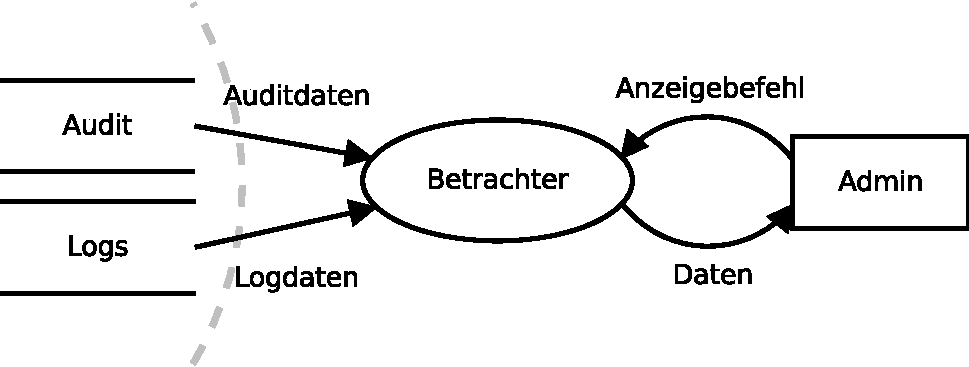
\includegraphics[scale=1.2]{images/dfd_logs.pdf}
\caption{DFD Log-/Audit-Datenfluss}
\label{fig:dfd_logs}
\end{figure}

\subsection{Gefährdungen identifizieren}

Die Protokollierung auf dem Marktrechner findet lokal statt, sodass die Aspekte der zentralen Protokollierung aus dem Baustein "Protokollierung" nicht betrachtet werden. Abbildung~\ref{fig:dfd_logs_threat} zeigt die Gefährdungen der einzelnen Beteiligten. Sabotage ist ein Aspekt, der bei Log- und Audit-Dateien gegeben ist, denn diese enthalten Informationen, die auf unerlaubte Aktivitäten schließen lassen. Versucht ein Angreifer, beispielsweise per Bruteforce-Angriff, das Passwort eines Benutzers herauszufinden, dann sind im Audit die fehlgeschlagenen Authentifizierungsversuche aufgezeichnet. Sollte dieser geglückt sein und der Benutzer hat Rechte das Audit zu verändern, kann der Angreifer seine Spuren verwischen. Ein anderer Angreifer könnte versuchen, Schwachstellen in der Implementierung zu finden. Im Log würden dadurch zahlreiche Fehlermeldungen entstehen. Durch Entfernen dieser kann er sicherstellen, dass eine eventuelle Sicherheitslücke unentdeckt bleibt. Der zweite Aspekt für Log- und Audit-Daten ist die Informationspreisgabe, da in beiden sensitive Daten enthalten sein können, welche Unberechtigte nicht einsehen dürfen. Der BSI hat diese Gefährung unter 2.161 "Vertraulichkeits- und Integritätsverlust von Protokolldaten" \cite{bsi_g2161} gelistet. Vertrauliche sensitive Informationen sind, beispielsweise Benutzername, IP-Adresse oder E-Mail. Falls Unberechtigte diese Daten einsehen können, entsteht dadurch eine neue Gefährdung, die der BSI unter 5.18 "Systematisches Ausprobieren von Passwörtern" benennt \cite{bsi_g5018}. Sollte ein Angreifer den Benutzernamen aus den vertraulichen Daten der Protokollierung erlangen, kann er diesen dazu nutzen, gezielt das Passwort zu erraten. Informationspreisgabe ist auch für die Betrachtungsfunktion zu berücksichtigen, diese darf Daten nur für Administratoren anzeigen. Zudem unterliegt sie der Personifikation, indem die eigentliche Betrachtungsfunktion mit Schadcode modifiziert wurde und nun vorgibt, die Ursprüngliche zu sein. Der BSI weist in 5.2 "Manipulation an Informationen oder Software" auf diese Gefährdung hin \cite{bsi_g5002}. Auch der Administrator unterliegt der Personifikation, indem ein Angreifer in Besitz der Berechtigungsnachweise kommt. Eine weitere Gefährdung bei Inhalten von Log- und Auditdaten wird durch die Bedrohungstunnelung verursacht \cite[s.~265]{gutmann}. Dabei wird Schadcode durch einen oder mehrere Instanzen getunnelt. Beispielsweise eine Anwendung, die bei jedem Anmeldeversuch den Benutzernamen protokolliert, kann zu einer Tunnelinstanz werden, indem ein Angreifer statt eines Benutzernamens Javascript-Schadcode angibt. Das Opfer des Angriffes ist eine Betrachtungsfunktion für die Protokollierung, welche die Inhalte in einer Web-Anwendung darstellt. Da die Web-Anwendung der protokollierenden Anwendung vertraut, werden die Inhalte nicht auf der Schadcode geprüft. Deshalb muss beachteten werden, dass die Daten zwar von vertrauenswürdigen Quellen kommen, die Inhalte allerdings aus nicht vertrauenswürdigen Quellen stammen. Unter diesem Gesichtspunkt muss eine Web-Anwendung in den Daten nach JavaScript-Inhalten suchen, auch wenn diese scheinbar von vertrauenswürdigen Quellen stammen.\footnote{Ein solcher Angriff wurde erfolgreich an https://github.com/nlaplante/syslogng-web durchgeführt}

\begin{figure}[htbp]
\centering
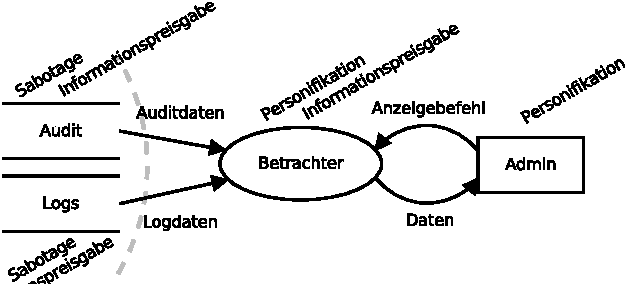
\includegraphics[scale=1.2]{images/dfd_logs_threats.pdf}
\caption{DFD Logdaten Gefährdungen}
\label{fig:dfd_logs_threat}
\end{figure}

\subsection{Maßnahmen}

Aus den Gefährdungen ergeben sich folgende Maßnahmen, welche zur Sicherung der Informationsflüsse durchgeführt werden müssen. Für Unix Systeme, unter welche Linux aus der Sicht des BSI fällt, hat der BSI die Maßnahme 4.25 "Einsatz der Protokollierung im Unix-System" erstellt \cite{bsi_m4025}. Diese weißt darauf hin, dass die Protokolldateien möglichst von Systemtools zu erstellen sind. Log- und Audit-Daten dürfen in einer Datei oder Datenbank abgelegt werden. Dabei weißt der BSI darauf hin, dass die Datei-Attribute ausschließlich dem Systembenutzer für Logging und Auditing modifizierende Rechte geben soll. Dabei wird angenommen, dass Datei-/Datenbankzugriffsmechanismus sowie Systemauthentifizierung nicht komprimiert sind. Der BSI empfiehlt für die Protokollierung mindestens folgende Ereignisse zu berücksichtigen: Logins (auch Fehlversuche), Aufruf von su, Fehlerprotokollierungsdatei / Protokollierung wichtiger Vorgänge (errorlog) und Administratortätigkeiten (insbesondere von root ausgeführte Befehle). Für die Alarmierung verweist der BSI zusätzlich noch auf halbautomatische Logfileparser des Systems, beispielsweise swatch, logsurfer oder checksyslog. Das Betrachten der Daten darf nur durch einen Administrator geschehen, der durch die Datei-Attribute ausschließlich lesend Zugriff erhält. In der Maßnahme 2.33 "Aufteilung der Administrationstätigkeiten unter Unix" weißt der BSI daraufhin, dass unter Linux Administratoren meist mit Super-User Rechten versehen werden \cite{bsi_m2033}. In diesem Fall ist es einem Benutzer möglich alle Dateien zu lesen, schreiben und auszuführen. Als eine mögliche Lösung werden daher spezielle Systembenutzer vorgeschlagen die Eigentümer von benötigten Programmen und Dateien sind. Für das Betrachten der Protokolldaten bedeutet dies, dass es einen Benutzer gibt der Rechte hat die Daten zu lesen und dessen Berechtigungsnachweis muss zwischen allen Administratoren des System ausgetauscht werden. Durch das Vermeiden von vielen Benutzern mit Super-User Rechten wird zudem das Risiko, dass die Betrachtungsfunktion von einem Angreifer modifiziert wurde gesenkt. Da die potentiellen Opferkandidaten reduziert wurden. Bei der Auswahl eines Administrators muss trotzdem mit besonderer Sorgfalt vorgegangen werden. Der BSI empfiehlt dies in der Maßnahme 3.10 "Auswahl eines vertrauenswürdigen Administrators und Vertreters" \cite{bsi_m3010}. Dort wird zudem darauf aufmerksam gemacht, dass der Administrator eine wichtige Schlüsselrolle ist und daher in seiner Abwesenheit genügend qualifizierte und natürlich auch vertrauenswürdige Vertreter vorhanden sein müssen. Ist die Betrachtungsfunktion eine Web-Anwendung, benötigt sie eine Authentifizierung, die mit der Systemauthentifizierung integriert ist. Log- und Audit-Daten müssen vor der Darstellung durch einen Sanitizer von schadhaften Inhalten befreit werden. Wurden solche Daten entfernt, muss der Administrator darauf hingewiesen werden. Der Administrator weist sich durch seinen Berechtigungsnachweis aus, dieser wird von ihm vor fremden Zugriff geschützt. Weiterhin erfolgt erneut die Annahme, dass die Systemauthentifizierung nicht komprimiert wurde. Als letzten Punkt der Maßnahme 4.25 empfiehlt der BSI die Sicherung der Protokollierung und verweist dabei auf gesetzliche und vertragliche Fristen.

\section{Benutzer-Anfragen} \label{sec:model_http}

Eingehende Benutzerverbindungen sollen ausschließlich über HTTPS erfolgen. Zu diesem Zweck wurde das RestGateway entwickelt, über welches auf den Marktrechner zugegriffen werden kann. 	

\subsection{Informationsfluss}

In Abbildung~\ref{fig:dfd_http} wird der Informationsfluss über das RestGateway gezeigt. Dabei fließen die Daten durch drei Vertrauensgrenzen. Sowohl RestGateway als auch LanGateway fungieren dabei als Datenproxy. Beide leiten die Anfragedaten ohne Validierung der Inhalte weiter. Deswegen muss darauf geachtet werden, dass ein Angreifer keine Bedrohungstunnelung durchführen kann. Das RestGateway arbeitet als Wrapper, unterschiedliche Abfragen werden anhand der URL unterschieden und in entsprechende TCP-CAN-Telegramme übersetzt. Die URL-Parameter einer Anfrage werden vom RestGateway auf einen gültigen Wertebereich überprüft. Die Antwort auf eine solche Anfrage sind menschenlesebare interpretierte Inhalte.

\begin{figure}[htbp]
\centering
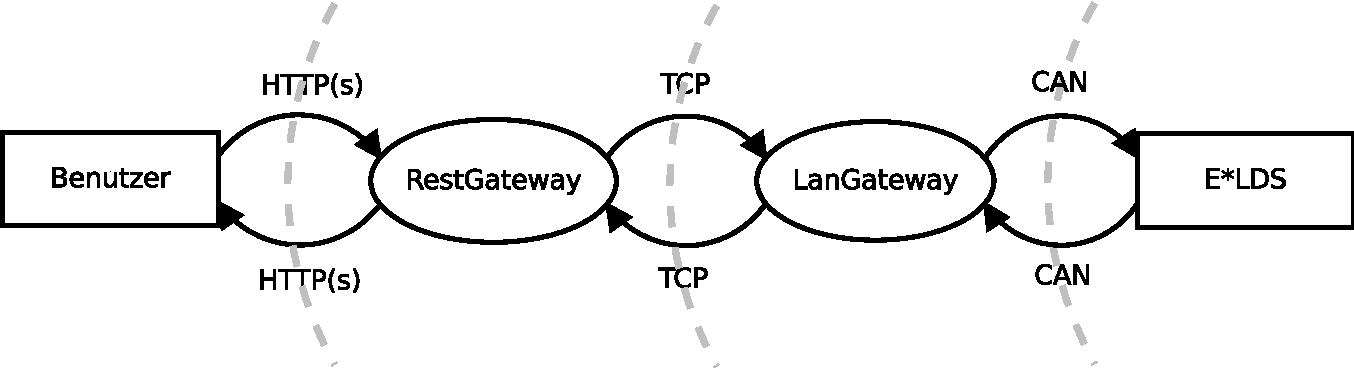
\includegraphics[scale=0.3]{images/dfd_http.pdf}
\caption{DFD HTTP-Anfrage}
\label{fig:dfd_http}
\end{figure}

\subsection{Gefährdungen identifizieren}

In Abbildung~\ref{fig:dfd_http_threat} sind die Bedrohungen in den fünf Kategorien aufgezeigt. Der Benutzer unterliegt der Gefahr der Personifizierung durch das Stehlen seines Berechtigungsnachweises. Dazu werden Phishing-Attacken genutzt, die bereits in Abschnitt~\ref{sec:attackers} ausführlich erläutert wurden. Ein Gefährdung durch Disput ist für den Benutzer ausgeschlossen, da die Log- und Audit-Daten nicht verändert werden können und der Zugriff zur Nachvollziehbarkeit im Audit dokumentiert ist. 

Auf dem Weg, den eine Benutzeranfrage zurücklegen muss, unterliegt diese an zwei Stellen der Möglichkeit einer Man-in-the-Middle-Attacke. Zunächst zwischen Benutzer und RestGateway und anschließend zwischen RestGateway und LanGateway. Durch einen MITM können an beiden Gateways Informationen preisgegeben werden, die der MITM mitliest. Zudem ist dieser auch in der Lage, die Inhalte zu sabotieren, anstatt die Informationen nur passiv mitzulesen. Auf Seiten des RestGateway sind die Informationen einfach zu interpretieren und daher einfach zu manipulieren. Ein MITM zwischen den beiden Gateways benötigt für die gleichen Aufgaben ein detailliertes Wissen über das Herstellerprotokoll. Ein dritter Angriffsvektor für den MITM ist, personifizierend aufzutreten. In der Personifikation als RestGateway kann der Angreifer eine Anfrage direkt an das LanGateway weiterleiten, wodurch eventuelle Sanatizer übergangen werden. Die Antwort des LanGateway kann er zudem beliebig sabotieren. Als LanGateway-Personifizierung ist er zwar nicht in der Lage, eine Nachricht an den CAN-Bus weiterzuleiten, kann jedoch dem Benutzer die Illusion einer erfolgreichen Kommunikation geben. Die Voraussetzungen sind hierbei die gleichen wie bei der Informationspreisgabe und Sabotage. Die verschieden Möglichkeiten eine MITM-Attacke durchzuführen, wurden in Abschnitt~\ref{sec:attackers} durch die verschiedenen Spoofing-Verfahren bereits detailliert erläutert.

Die Funktionen RestGateway und LanGateway unterliegen durch ihre Netzwerkschnittstellen der Gefahr einer DoS-Attacke. Während das RestGateway über das Internet kontaktiert werden kann, ist das LanGateway nur über das LAN zu erreichen. Das LAN obliegt der Kontrolle der Endkunden, daher liegt das Risiko alleine beim Endkunden und wird nicht weiter betrachtet. Auf die Gefährdungen durch DoS-Attacken wurde bereits ausführlich in Abschnitt~\ref{sec:attackers} eingegangen. Ziele die ein Angreifer durch die Überlastung des Marktrechners verfolgen kann, sind, Verhinderung der Datenarchivierung, der Alarmierung und der Überwachung der Anlage. Anlagenschaden kann er damit nicht anrichten, da alle Komponenten der Kälteanlage über einen Notmodus, ohne den Marktrechner arbeiten können. Bei der Beschreibung einer Kälteanlage wurde zudem gesagt, dass die Prozesse, um Warenschaden anzurichten, nur langsam voranschreiten. Aus diesem Grund wird ein Monteur die Anlage höchstwahrscheinlich wieder instand setzen, bevor Schaden entsteht, da der Angriff auf jeden Fall entdeckt wird.

\begin{figure}[htbp]
\centering
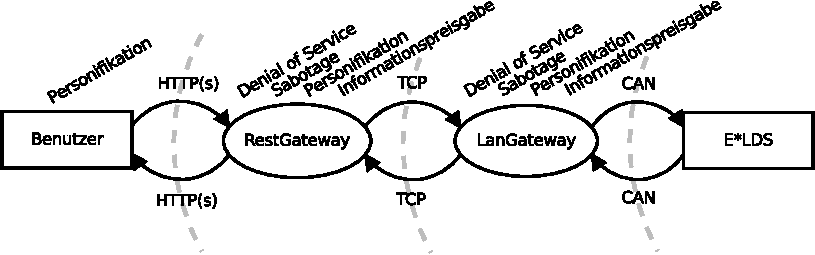
\includegraphics[scale=1]{images/dfd_http_threat.pdf}
\caption{DFD HTTP-Gefährdungen}
\label{fig:dfd_http_threat}
\end{figure}

\subsection{Maßnahmen}

An Berechtigungsnachweise von Benutzern zu gelangen, ist für einen motivierten Angreifer durch Phishing-Attacken möglich. Unter dieser Annahme wird festgelegt, dass ungewöhnliche Login-Muster in den Audit-Daten erkannt werden müssen, beispielsweise wenn sich ein Benutzer innerhalb weniger Minuten von unterschiedlichen physikalischen Orten verbindet. Um RestGateway und LanGateway durch einen Man-in-the-Middle zu schützen, wurde bereits in Abschnitt~\ref{sec:attackers} festgelegt, auf DNS-Adressen zu verzichten \cite{bsi_m5059}. Diese Anforderung ist jedoch problematisch, wenn es um die Flexibilität einer IT-Infrastruktur geht. Deshalb können DNS-Adressen eingesetzt werden, wenn bei der Konfiguration des DNS-Servers sorgfältig vorgegangen wird. Die Gefährdung durch eine Fehlkonfiguration wird durch eine menschliche Fehlhandlung verursacht und deshalb in diesem Rahmen nicht weiter betrachtet. Ein 100-prozentiger Schutz gegen einen MITM ist daher nicht zu gewährleisten. Der Authentifizierungsmaßnahmen des BSI für einen Schutz gegenüber Phishing-Attacken, ist leider nicht existent. Damit ein Angreifer, der über eine Phishing-Attacke an den Berechtigungsnachweis eines Benutzers gelangt ist, trotzdem keinen Zugriff auf das System erlagen kann, soll eine Zwei-Faktor-Authentifizierung (2FA) eingesetzt werden. Eine 2FA benötigt zur erfolgreichen Authentifizierung eines Benutzers zwei Komponenten. Zum einen etwas, was der Benutzer weiß und zum andern etwas, was der Benutzer besitzt. Die erste Anforderung wird durch das Wissen von Benutzername und Passwort bereits erfüllt. Für die zweite Anforderung muss sich der Benutzer durch Client-Zertifikat ausweisen. Bei der 2FA findet zunächst eine Zertifikatsüberprüfung statt, dabei überprüft der Client das Server-Zertifikat und vice versa. Aus Gründen der Benutzerfreundlichkeit wird das Client-Zertifikat auf den Endgeräten der Benutzer installiert, wodurch die Überprüfung für diese transparent funktioniert. Im nächsten Schritt weist sich der Benutzer aktiv durch seinen Berechtigungsnachweis aus. Auf diesem Weg wird verhindert, dass von unautorisierten Geräten auf den Marktrechner zugegriffen werden kann. Dadurch wird das Risiko einer MITM-Attacke, verglichen mit Aufwand und Kosten, auf ein akzeptables Niveau gesenkt. Durch den Einsatz von Zertifikaten entsteht allerdings das Risiko durch die Gefährdung 5.84 "Gefälschte Zertifikate" \cite{bsi_g5084}. Hier muss darauf geachtet werden, dass Zertifikate auch geprüft werden und das kein Mitarbeiter absichtlich oder fälschlicherweise beliebig Zertifikate generieren kann. Weitere Details zur Schlüsselverwaltung werden im nächsten Abschnitt, anhand der Schlüsselkontinuität, erläutert.

Die Authentifizierung, welche in Abschnitt~\ref{sec:analysis_measures} gefordert wird, muss über drei Vertrauensgrenzen sichergestellt werden. Bei jedem Durchschreiten einer Vertrauensgrenze besteht das Risiko attackiert zu werden. Um die Quellen für Gefährdungen durch zu viele Vertrauensgrenzen zu reduzieren, sollte die Funktionalität des LanGateway in das RestGateway integriert werden. Ein externes RestGateway würde anstatt des LanGateway mit dem internen RestGateway kommunizieren, welches dann lediglich als Proxy fungiert. Alternativ muss sichergestellt werden, dass das LanGateway ausschließlich lokal über die Loopback-Adresse (127.0.0.1) erreichbar ist. Aufgrund der Gefahr durch Bedrohungstunnelung muss jede Funktion, die für sich relevanten Eingaben von einem Sanatizer prüfen lassen.

\section{M2M-Kommunikation} \label{sec:model_auth}

Die Authentifizierung und Autorisierung wird vom Marktrechner an einen AAS-Server ausgelagert. Für diesen Abschnitt ist der Baustein 1.7 "Kryptokonzept" aus der Kategorie Übergreifende Aspekte von Bedeutung \cite{bsi_b1017}.

\subsection{Informationsfluss}

In Abbildung~\ref{fig:dfd_auth} wird der Informationsfluss zwischen Marktrechner und AAS dargestellt. Eingeleitet wird der Informationsfluss stets vom Marktrechner, wenn dieser eine Benutzeranfrage erhält und den Berechtigungsausweis validieren möchte. Als Antwort erhält er das Validierungsergebnis und für den Erfolgsfall, die Rollen des Benutzers. Alternativ kann der Marktrechner den Berechtigungsnachweis in Verbindung mit einer Rolle an den AAS senden. Ein positives Validierungsergebnis sagt dann aus, dass der Berechtigungsnachweis gültig ist und der Benutzer die geforderte Rolle inne hat. Dies kann, beispielsweise für eine mehrstufige Autorisierung lokal am Marktrechner genutzt werden, da hier die Einstellungen über die GUI in mehreren Ebenen organisiert sind. Die eigentlichen Module, beispielsweise das RestGateway, wurden in der Abbildung der Einfachheit wegen in Marktrechner und AAS abstrahiert. Bevor die Validierung erfolgen kann, muss zunächst eine authentifizierte Verbindung vom Marktrechner zum AAS hergestellt werden.

\begin{figure}[htbp]
\centering
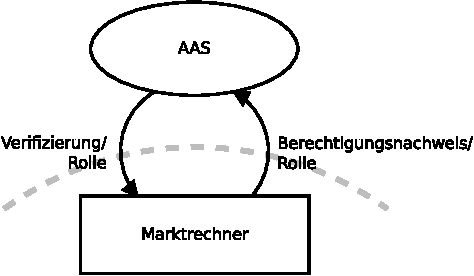
\includegraphics[scale=1.1]{images/dfd_auth.pdf}
\caption{DFD Authentifizierung-Autorisierung}
\label{fig:dfd_auth}
\end{figure}

\subsection{Gefährdungen identifizieren}

Die Gefährdungen wurden in Abbildung~\ref{fig:dfd_auth_threat} visualisiert. Sowohl Marktrechner als auch AAS unterliegen der Gefährdung der Personifikation. Die Verbindung zwischen den beiden Teilnehmern ist über ein Public/Private-Key Verfahren abgesichert. Dabei weist der BSI auf die Gefährdung 4.35 "Unsichere kryptographische Algorithmen" hin \cite{bsi_g4035}. Hierbei muss darauf geachtet werden, dass ein Angreifer nicht mit vertretbaren Ressourcen das kryptographische Verfahren brechen kann. Des Weiteren besteht die Gefahr 2.19 "Unzureichendes Schlüsselmanagement bei Verschlüsselung" \cite{bsi_g2019}. Ein ungeeignetes Schlüsselmanagement identifiziert der BSI an:

\begin{itemize}
\item kryptographischen Schlüssel die in einer ungesicherten Umgebung erzeugt oder aufbewahrt werden,
\item ungeeignete oder leicht erratbaren Schlüsseln,
\item zur Verschlüsselung bzw. Entschlüsselung eingesetzten Schlüssel, die den Kommunikationspartner nicht auf einem sicheren Weg erreichen.
\end{itemize}

Davon abgeleitet wird die Gefährdung 5.83 "Kompromittierung kryptographischer Schlüssel" \cite{bsi_g5083}. Bei Verfahren mit kryptographischen Schlüsseln hängt die Sicherheit maßgebend davon ab, dass diese geheim bleiben. Ein Beispiel der Kompromittierung, neben dem Schlüsselmanagement, ist das entwenden, der als Backup hinterlegten Schlüssel. Dadurch entsteht die Gefährdung der Informationspreisgabe am AAS. Ein Angreifer könnte sich als Marktrechner ausgeben und versuchen, über Bruteforce oder sonstige Verfahren das Passwort eines Nutzers herauszufinden.

Der Marktrechner unterliegt zudem der Gefährdung einer DoS-Attacke, da er jedoch derjenige ist, der die Verbindung initialisiert und eingehende Verbindungen nicht zugelassen werden, ist das Risiko bei der M2M-Kommunikation zu vernachlässigen.

\begin{figure}[htbp]
\centering
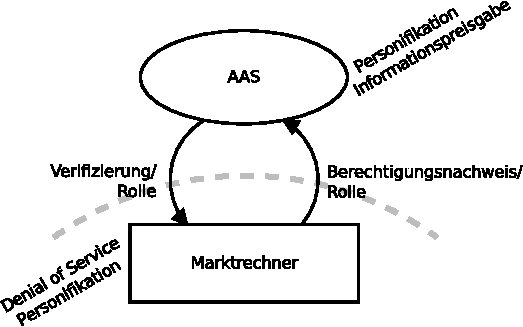
\includegraphics[scale=1.1]{images/dfd_auth_threat.pdf}
\caption{DFD Authentifizierung-Autorisierung}
\label{fig:dfd_auth_threat}
\end{figure}

\subsection{Maßnahmen}

Die Kryptographie von Authentifizierungslösungen wurde vor Jahrzehnten entworfen und ist dementsprechend erprobt. Die Auswahl eines geeigneten Verfahrens beschreibt das BSI in der Maßnahme 2.164 "Auswahl eines geeigneten kryptographischen Verfahrens" \cite{bsi_m2164}. Bei symmetrischen Verfahren, wie AES oder SERPENT, soll eine Mindestschlüssellänge von 100-Bit gewählt werden. Bei asymmetrischen Verfahren eignet sich RSA oder auf Elliptischen Kurven basierende Verschlüsselungsverfahren. Als Schlüssellänge für RSA wird mindestens 1536-Bit gefordert. Damit die Kryptographie funktioniert, müssen Schlüssel ausgetauscht werden. Das BSI hat in der Maßnahme 2.46 "Geeignetes Schlüsselmanagement" sinnvolle Hinweise für die einzelnen Aufgaben des Schlüsselmanagements zusammengestellt. Zunächst müssen die Schlüssel generiert werden, das soll in einer sicheren Umgebung und unter dem Einsatz geeigneter Schlüsselgeneratoren erfolgen. Die primäre Problemstellung bei der Schlüsselverwaltung ist allerdings: Wie gelangt ein Schlüssel vom Erzeuger, zu den vorgesehenen Empfängern? Das populärste Modell der Schlüsselverteilung ist das "Schlüssel fallen aus dem Himmel"-Modell. Es ist deshalb so weit verbreitet, weil durch die Komplexität des Problems, Entwickler von Sicherheitsprotokollen es gerne ignorieren und jemand Anderem die Lösungsfindung zuschieben. Das BSI macht hierzu keinen Lösungsvorschlag, es gibt lediglich den banalen Hinweis, die Schlüssel nicht unverschlüsselt zu übertragen, sondern entsprechende Verfahren, beispielsweise Key Encryption Key (KEK) bei X.509-Zertifikaten, zu verwenden. Ein Konzept das nicht dem "Schlüssel fallen aus dem Himmel"-Modell unterliegt, ist das der Schlüsselkontinuität \cite{ietf_kcm}. Implementiert wird dieses, beispielsweise in SSH oder PGP. Ihm zugrunde liegt das Konzept der Beständigkeit, dass bedeutet, anhand des Schlüssel kann überprüft werden, ob die Entität, mit welcher gestern kommuniziert wurde, auch heute noch dieselbe ist. Die Schlüsselkontinuität unterliegt allerdings einer Schwachstelle, denn beim initialen Austausch ist eine MITM-Attacke möglich. Ein Angreifer hat dementsprechend exakt eine Chance die Verbindung zu kompromittieren. Wenn er zu diesem Zeitpunkt die Attacke nicht durchführen kann, hat er seine Chance vertan. Ein derartiger Angriff ist nicht auszuschließen, jedoch ist das Wahrscheinlichkeit sehr gering und daher das Risiko für die M2M-Kommunikation akzeptable. Sollte in Zukunft entschieden werden, dass das Risiko eines MITM während des initialen Schlüsselaustausches nicht tragbar ist, können Fingerprints der öffentlichen Schlüssel oder Zertifikate ausgetauscht werden. Der Austausch von Fingerprints muss natürlich auf einem alternativen Kommunikationskanal erfolgen. Hierzu empfiehlt sich der Versandweg per Post oder Kurier. Beim Versand des verifizierenden Datenträgers gilt jedoch Vorsicht. Der BSI hat für die Versendung von Datenträgern eine Maßnahme verfasst. Unter 5.23 "Auswahl einer geeigneten Versandart für Datenträger" listet der BSI vier Möglichkeiten für den Versand \cite{bsi_m5023}: Post, Kurierdienste, persönlicher Kurier oder persönliche Übergabe. Für den Austausch von Datenträgern, die die Identität von AAS und Marktrechner bescheinigen, sollte die persönliche Übergabe gewählt werden. Hierbei wird ein vertrauenswürdiger Kurier, etwa ein Mitarbeiter, mit dem Datenträger gesendet und übergibt diesen persönlich dem dafür bestimmten Empfänger. Während der Übergabe bekommt der Kurier auch den Datenträger des Anderen, wodurch eine gegenseitige Authentifizierung möglich wird. Diese Maßnahme ist die sicherste, aber auch die teuerste. Ob eine FSZ statt eines persönlichen Kuriers die Post einsetzt, hängt von der eigenen Risikobewertung ab, der Hersteller kann hier nur eine Empfehlung aussprechen. Nach dem initialen Schlüsselaustausch besteht für den MITM eine weitere Möglichkeit die Verbindung zu komprimierten und zwar während eines Schlüsselwechsels. In einer Sicherheitsrichtlinie muss festgelegt werden, wie oft dies Vorkommen soll, dabei gibt es keine Richtwerte von Seiten des BSI. Ein ausgetauschter Schlüssel muss gespeichert werden. Unter dem Punkt Schlüsselinstallation und -speicherung, weist das BSI daraufhin, dass zumindest Zeitweise die Schlüssel im Klartext verfügbar sind. Kann dem System nicht vertraut werden, empfiehlt sich die Auslagerung auf Hardware-Verschlüsselungskomponenten. Letzter Teil der Schlüsselverwaltung ist die Schlüsselvernichtung. Hierbei muss sichergestellt werden, dass ein Schlüssel wirklich entfernt wurde, etwa durch mehrfaches überschreiben der Speicherzellen auf einem Datenträger.

\chapter{Prototypische Implementierung} \label{chap:implementation}

In diesem Kapitel wird eine prototypische Implementierung, anhand der in den vorherigen Kapiteln besprochenen Maßnahmen gezeigt. Zunächst werden Kriterien festgelegt, die die prototypische Implementierung erfüllen soll. Als Leitfaden dienen die Security Assurance Requirements (SAR) aus dem Protection Profile der Common Criteria. Diese definieren in einer standardisierten Sprache die notwendigen Aufgaben für die verschiedenen Stufen der Vulnerability Analysis (AVA\_VAN).

\section{Schlüsselwörter}

In diesem Abschnitt werden die folgenden Schlüsselwörter definiert, welche als Hilfe zur Bewertung bei der Evaluierung dienen. Die Schlüsselwörter und deren Bedeutung orientieren sich an dem Request For Change (RFC) 2119 der Internet Engineering Task Force (IETF) \cite{rfc_2119}:

\begin{center}
\textit{"MUSS", "SOLL", "ERFORDERLICH", "DARF" "EMPFOHLEN", "NICHT", "KANN" und "OPTIONAL"}
\end{center} 

\begin{enumerate}
\item \textbf{MUSS}~~~~Dieses Wort oder die Terme "SOLL" und "ERFORDERLICH" bedeuten, dass eine  Definition unverzichtbarer Teil einer Spezifikation sein soll.
\item \textbf{SOLL NICHT}~~~~Diese Phrase bedeutet ein Verbot einer Definition als Teil einer Spezifikation.
\item \textbf{DARF}~~~~Dieses Wort oder das Adjektiv "EMPFOHLEN" bedeuten, dass es  Gründe gibt, warum unter besonderen Umständen, auf diese Definition als Teil einer Spezifikation verzichtet werden darf. 
\item \textbf{DARF NICHT}~~~~Diese Phrase bedeutet, dass auf ein Verbot, einer Definition als Teil einer Spezifikation, unter besonderen Umständen verzichtet werden darf.
\item \textbf{KANN}~~~~Dieses Wort oder der Term "OPTIONAL" bedeuten, dass diese Definition als Teil einer Spezifikation nach belieben umgesetzt werden darf.
\end{enumerate}

\section{Anforderungen}

Die folgenden Anforderungen, werden an die prototypische Implementierung gestellt. Diese soll Benutzer authentifizieren und autorisieren können. Die Anforderungen an Log- und Audit-Mechanismus werden der Vollständigkeit halber erfasst. Aufgrund des Aufwandes in der prototypischen Implementierung jedoch nicht weiter berücksichtigt.

\subsection{Log-/Audit-Mechanismus}

Das System \textit{MUSS} einen Audit-Mechanismus implementieren, der Zugriffe \textit{SOLL} zumindest mit Benutzername, IP-Adresse, Zeitstempel und Häufigkeit protokolliert werden. Des Weiteren \textit{DARF} das System \textit{NICHT} Informationen protokollieren, die sensitive Daten oder datenschutzrechtlich illegal Inhalte beinhalten. Das System \textit{KANN} ein Frühwarnsystem haben, welches die Audit-Daten überwacht, ist dies nicht der Fall \textit{MUSS} die Möglichkeit bestehen, die Audit-Daten in Echtzeit mitzuverfolgen, um ein eigenes Frühwarnsystem zu installieren.

\subsection{M2M-Kommunikation}

Das System \textit{DARF} beidseitige asynchrone Authentifizierung unterstützten, die dabei genutzte Kryptographie \textit{DARF} der Perfect Forward Security genügen. Das System \textit{KANN} die Schlüsselkontinuität implementieren, ist dies nicht der Fall \textit{MUSS} der Authentifizierungsmechanismus erweiterbar sein. \textit{OPTIONAL} können Fingerprints der Schlüssel beziehungsweise Zertifikate getauscht werden. Beim Austausch der Fingerprints ist es \textit{ERFORDERLICH}, dass der Austauschkanal ein Anderer ist, wie der Kommunikationskanal.

\subsection{Benutzer-Kommunikation}

Der Benutzer wird zunächst eine Verbindung mit dem Marktrechner aufbauen. Der Marktrechner \textit{MUSS} das Client-Zertifikat prüfen, bevor eine Verbindung aufgebaut wird. Der Benutzer teilt anschließend seinen Berechtigungsnachweis mit. Anhand dessen bittet der Marktrechner das AAS-System um Validierung. Die Validierung \textit{MUSS} zu einem Ergebnis Berechtigungsnachweis gültig oder Berechtigungsnachweis ungültig kommen. Neben den Validierungsergebnis \textit{SOLL(EN)} die Rolle(n) des Benutzers an den Marktrechner geprüft oder übermittelt werden.

\section{Analyse}

Für die prototypische Implementierung wurden vor Beginn der Thesis zwei Softwareprodukte herausgesucht, die anhand ihrer Beschreibungen zu dem Thesis-Thema passten. In diesem Abschnitt, sollen die beiden Produkte anhand der Anforderungen auf Umsetzbarkeit geprüft werden. Zunächst wird die Middleware CodeMeter der Wibu-Systems AG betrachtet und anschließend der Open-Source RADUIUS-Server FreeRADIUS.

\subsection{CodeMeter}

CodeMeter ist die Middleware der Wibu-Systems AG, deren Hauptaufgabe der Softwareschutz und das Lizenzmanagement ist. Auf speziell geschützten USB-Sticks, den sogenannten Wibu-Keys, werden daher hauptsächlich Schlüssel für Softwarelizenzensierung verteilt. Es ist allerdings möglich beliebige Daten sicher durch die Wibu-Keys zu verteilen, beispielsweise Client-Zertifikate für die Benutzer-Kommunikation. Für WAN-Verbindungen sieht die Entwickler-Dokumentation folgende Architektur vor:

\begin{figure}[htbp]
\centering
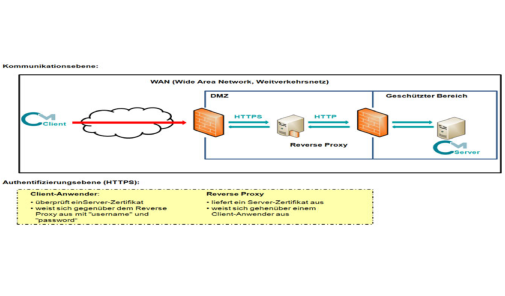
\includegraphics[scale=1.2]{images/codemeter_wan.pdf}
\caption{CodeMeter WAN-Architektur}
\label{fig:radius_access}
\end{figure}

Über HTTPS stellt ein CodeMeter-Client eine Anfrage. Diese muss von einem Reverse Proxy entgegengenommen werden. Dieser liefert daraufhin ein Server-Zertifikat aus, dass der Client überprüft. Optional kann der Reverse Proxy den Kunden durch Benutzername und Passwort authentifizieren. Client-Zertifikate werden, zum Zeitpunkt des Schreibens dieser Thesis, nicht von der CodeMeter-Software unterstützt. Des Weiteren gehört der Reverse-Proxy, sowie die Art und Weise der Benutzerauthentifizierung nicht zum Funktionsumfang der CodeMeter-Software. 

\subsection{FreeRADIUS}

RADUIS ist ein Authentifizierungsdienst für sich einwählende Benutzer (engl. Remote Authentication Dial-In User Service). Er besteht aus einem Client-Server-Protokoll zur Authentifizierung, Autorisierung und Buchhaltung (engl. Accounting). Dieses sogenannte Triple-A-System wird hauptsächlich bei VPN, WLAN oder DSL genutzt. Beispielsweise wird das weltweite eduroam-Netzwerk, dass Studierenden und Mitarbeitern von Hochschulen erlaubt einen WLAN-Internetzugang, an allen Standorten teilnehmender Organisationen, anhand ihres eigeneeduroamn Berechtigungsnachweises, zu erhalten. Der Accounting-Aspekt von RADIUS ist nicht Teil dieser Thesis und wird deshalb vernachlässigt. RADUIS selbst besitzt nur eine sehr einfach Konfigurationsdatenbanken zur Authentifizierung. Aus diesem Grund können moderne RADIUS-Server diese Funktionalität an gängige Authentifizierungsserver, beispielsweise SQL-Datenbanken, Kerberos, LDAP oder Active Directory, delegieren. Ein RADIUS-Server kann daher als Multiplexer eingesetzt werden, um verschiedene externe Authentifizierungsserver mit einem Protokoll zu anzusprechen.

Das RADIUS-Protokoll zur Authentifizierung läuft in zwei Phasen ab (Abbildung~\ref{fig:radius_access}). Zunächst sendet ein RADIUS-Client einen Access-Request, welcher von einem RADIUS-Server entweder mit Access-Accept, für eine erfolgreiche Authentifizierung, oder Access-Reject, für einen fehlerhafte Authentifizierung, beantwortet wird. Die dritte Möglichkeit Access-Challange wird für komplexere Authentifizierung genutzt, um zusätzliche Informationen abzufragen, beispielsweise ein zweites Passwort oder einen Token. Für den Rahmen der prototypischen Implementierung wird diese Möglichkeit nicht weiter betrachtet. Alle Attribute einer RADIUS-Nachricht, beispielsweise Benutzer oder Passwort, bestehen aus Attribute-Value-Pairs (AVP). Neben im Protokoll vorgeschriebenen gibt es herstellerspezifische und benutzerdefinierte Attribute. RADIUS-Client und RADIUS-Server verschlüsseln die AVPs anhand eines beiden bekannten Geheimnisses.

\begin{figure}[htbp]
\centering
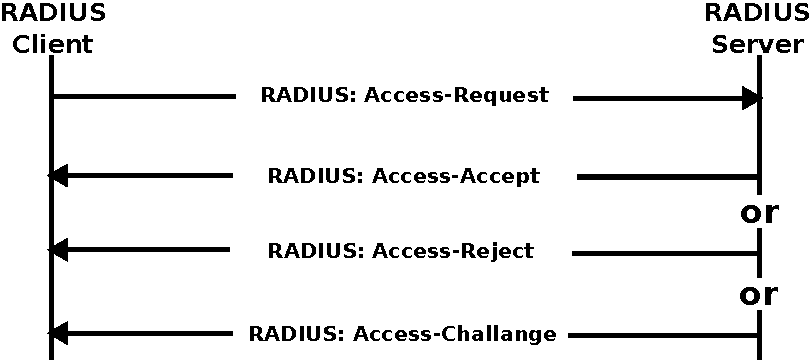
\includegraphics[scale=0.8]{images/RADIUS_access.pdf}
\caption{RADUIS Access-Protokoll}
\label{fig:radius_access}
\end{figure}

Der FreeRADIUS-Server besitzt zudem eine Richtliniensprache, welcher er zur Umsetzung einer rollenbasierten Autorisierung nutzen kann. Damit ist er in der Lage Attribute-Value-Pairs auszuwerten und das Ergebnis der Authentifizierung zu manipulieren. Der FreeRadius-Server kann unter Windows, Mac, Linux und BSD Systemen aufgesetzt werden. Die Client-Library läuft wenigsten unter Linux, was für den Einsatz auf dem Marktrechner ausreichen ist.

\subsection{Schlussfolgerung}

\paragraph{CodeMeter}

Die Wibu-Keys können für die sichere Verteilung der Client-Zertifikate genutzt werden, die für die Benutzer-Kommunikation nötig sind. Die CodeMeter-Software ist allerdings, zum Zeitpunkt des Schreibens dieser Thesis, unbrauchbar, da Sie keine Client-Zertifikat unterstützt, was die Anforderung an die Benutzerkommunikation verletzt. Ob der Einsatz von Wibu-Keys zur Verteilung von Client-Zertifikaten wirtschaftlich ist, muss gesondert von der Firma ECKELMANN evaluiert werden. Für die prototypische Implementierung wird die CodeMeter-Software daher nicht eingesetzt.

\paragraph{FreeRADIUS}

Der Marktrechner ist in der Lage mit Hilfe der Client-Library den FreeRADUIS-Server zur Authentifizierung und Autorisierung zu kontaktieren. Durch die Multiplexer Funktionalität sind zudem die meisten Authentifizierungsserver abgedeckt, welche eine Fernservice-Zentrale zur Verwaltung ihrer Benutzer nutzen könnte. Dadurch ist der FreeRADUIS-Server bestens geeignet die Authentifizierung und die Autorisierung für den Marktrechner durchzuführen. Lediglich die Authentifizierung und Verschlüsselung zwischen Client und Server auf Basis des geteilten Geheimnisses erfüllt nicht die Anforderungen. Weder KCM noch PFS können hierbei unterstützt werden, noch ist der Mechanismus erweiterbar. Unter diesen Bedingungen erhält der Einsatz eines RADIUS-Server die Auflage, das Anfragen nicht über das Internet gestellt werden sollen, da das Risiko dort angegriffen zu werden zu hoch ist. Trotz dieser Einschränkung ist der FreeRADIUS-Server eine sinnvolle Lösung und soll deshalb für die prototypische Implementierung aufgesetzt werden.

\section{Prototyp}

In diesem Abschnitt wird zunächst das Konzept für die prototypische Implementierung beschrieben. Anschließend wird auf die Konfiguration der Komponenten für die Benutzer-Kommunikation und M2M-Kommunikation eingegangen. Zum Schluss wird die eigentlich Implementierung erläutert.

\subsection{Konzept}

Das Konzept der prototypischen Implementierung ist zweigeteilt. Auf der einen Seite die Benutzer-Kommunikation zum Marktrechner hingehend und auf der anderen Seite die Authentifizierung und Autorisierung vom Marktrechner ausgehend. In der Abbildung~\ref{fig:konzept_proto_impl} sind alle Komponenten gezeigt.

\begin{figure}[htbp]
\centering
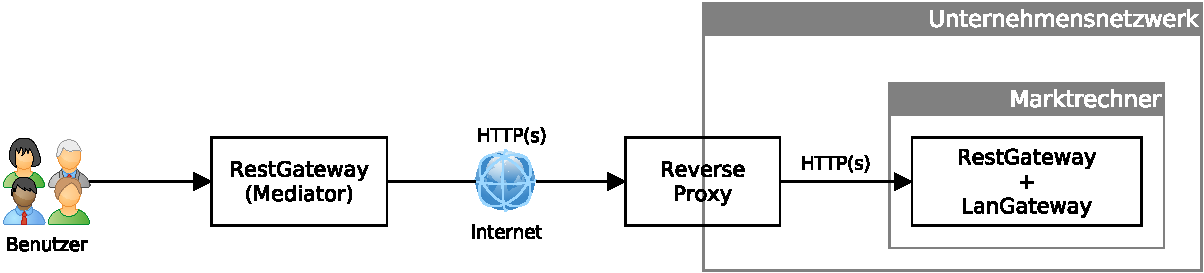
\includegraphics[scale=1]{images/design_architekture.pdf}
\caption{Konzept prototypische Implementierung}
\label{fig:konzept_proto_impl}
\end{figure}

Für die Benutzer-Kommunikation wird als Client der Firefox-Browser eingesetzt. Dieser stellt seine Anfrage gegen den Reverse Proxy, welcher durch einen lighttpd-Webserver realisiert wird. Nach erfolgreicher Zertifikatsprüfung wird eine Anfrage an den Marktrechner weitergeleitet. Das RestGateway-Modul entnimmt Benutzername und Passwort aus den Anfrageparametern. Mit Hilfe der FreeRADIUS-Client-Library sendet es eine Access-Request-Nachricht an den FreeRADIUS-Server. Der RADIUS-Server delegiert die Authentifizierung an den LDAP-Server ApacheDS und führt anschließend eine rollenbasierte Autorisierung durch. Im Erfolgsfall sendet er eine Access-Accept-Nachricht, ansonsten eine Access-Reject-Nachricht. Dementsprechend beantwortet der Marktrechner die Benutzeranfrage mit dem Anfrage-Ergebnis oder dem HTTP-Fehlercode 503 (Forbidden).

\subsection{Benutzer-Kommunikation}

Bevor mit dem Benutzer kommuniziert werden kann muss ein Client-Zertifikat erstellt werden. Dazu wird die openssl-Biblithek verwendet ... eigene CA ... 

Das Client-Zertifikat im p12-Format kann nun im Firefox-Browser hinzugefügt werden. Über den folgenden Aufruf, sendet der Benutzer eine Anfrage an den Reverse-Proxy.

\begin{lstlisting}[caption=HTTPS-Anfrage an Reverse Proxy, label=lst:https_request]
https://marktrechner.eckelmann.de/rest/1.0/controller?user=ksapp&pass=123456
\end{lstlisting}

Der Reverse-Proxy lässt ausschließlich HTTPS-Anfragen zu. Erfolgt ein HTTP-Aufruf, wird dieser nach HTTPS gezwungen. Der Reverse Proxy liefert daraufhin sein selbst signiertes Server-Zertifikat aus und fordert das mit diesem signierte Client-Zertifikat an. Dies geschieht vollkommen transparent für den Benutzer. Im Falle einer erfolgreichen Authentifizierung des Client-Zertifikates wird die Anfrage an den Marktrechner weitergeleitet.

\subsection{M2M-Kommunikation}

Zur Benutzerauthentifizierung wird eine Benutzerverwaltung benötigt. Das Lightweight Directory Access Protocol (LDAP) wird von den meisten Benutzerverwaltungen unterstützt und soll deshalb hier genutzt werden. Eine Benutzerverwaltung die dieses Protokoll unterstützt, ist der ApacheDS-Server. LDAP legt Daten in einer Baumstruktur ab. Für eine Benutzerverwaltung gibt es jedoch keine Vorgaben, wie die Baumstruktur anzulegen ist. Jeder Knoten kann von beliebig vielen Objekt-Klassen erben. Anhand der Objekt-Klassen sind Attribute verfügbar, die teilweise verpflichtend sind. 
\begin{figure}[htbp]
\centering
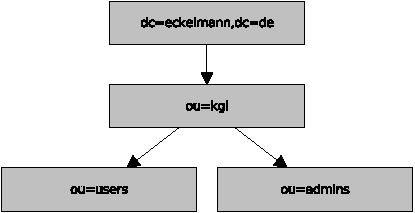
\includegraphics[scale=1]{images/ldap_structure.pdf}
\caption{LDAP Struktur}
\label{fig:ldap_sturcture}
\end{figure}
In Abbildung~\ref{fig:ldap_sturcture} ist die Struktur dargestellt, die für die prototypische Implementierung gewählt wurde. Vom root-Knoten, mit den Domain Components \textit{dc=meinedomain,dc=local}, ausgehend, wurden drei Kinderknoten, die von der Objekt-Klasse \textit{organizationalUnit} erben, erzeugt. Diese Objekt-Klasse verpflichtet zur Angabe des Namens der Unternehmenseinheit (\textit{ou}). Zunächst wurde die Einheit \textit{radius} gewählt, welche die Untereinheiten \textit{users} und \textit{admins} hat. Diese beiden beinhalten jeweils Benutzerknoten.

Der Benutzerknoten, in Auflistung~\ref{lst:ldif_user} im LDIF-Format dargestellt, erbt von zwei Objekt-Klassen. Der Distinguished Name (\textit{dn}) erlaubt es einen Knoten eindeutig im Baum zu finden. Über die Objekt-Klasse \textit{person} wird verpflichten das Attribut Common-Name (\textit{cn}) verfügbar, sowie weitere optionale Attribute für Vorname, Nachname, Benutzername und Passwort. Der Benutzername wird über uid angegeben und spielt eine wichtige Rolle für die spätere FreeRADIUS-Konfiguration. Die Objekt-Klasse \textit{radiusProfile} ermöglicht das hinzufügen von Rollen, die der FreeRADIUS-Server als \textit{radiusGroupName}-Attribute kennt und auslesen kann.

\begin{lstlisting}[caption={Benutzerbeschreibung im LDIF-Format},label=lst:ldif_user]
dn: cn=Kevin Sapper,ou=users,ou=radius,dc=meinedomain,dc=local
objectClass: top
objectClass: radiusProfile
objectClass: person
cn: Kevin Sapper
givenName: Kevin
sn: Sapper
uid: ksapp
userPassword:: e3NoYX1mRXFOQ2NvM1lxOWg1WlVnbEQzQ1pKVDRsQnM9
radiusGroupName: analyst
radiusGroupName: fernservice
\end{lstlisting}

Der komplette Inhalt des LDAP-Server, im LDIF-Format, ist im Anhang zu finden. 

Die Konfiguration des FreeRADIUS-Server beginnt mit dem Einrichten der LDAP-Verbindung. Zunächst muss eine Verbindung mit dem LDAP-Server aufgebaut werden. Der FreeRADIUS-Server loggt sich dazu über den Berechtigungsnachweis eines Benutzers, der Unternehmenseinheit \textit{admins}, ein. Über das \textit{identity}-Attribute wird dieser Benutzer angegeben. Für die prototypische Implementierung wurde hierzu der Benutzer \textit{cn=binduser} angelegt. Damit die Admin-Benutzer nicht für die allgemeine Authentifizierung genutzt werden können, wird die Unternehmenseinheit \textit{users} Basisknoten, über das \textit{basedn}-Attribute festgelegt. Valide Benutzerknoten erben von der \textit{radiusprofile} Objekt-Klasse und besitzen das \textit{uid}-Attribute für den Benutzernamen. Findet der FreeRADIUS-Server einen übereinstimmenden Benutzernamen, liest er dessen Passwort aus und vergleicht es mit dem übermittelten. Ist dies erfolgreich markiert der FreeRADIUS-Server den Access-Request mit \textit{accept} und liest er die Rollen des Benutzers über die \textit{radiusGroupName}-Attribute aus.

Bevor ein Marktrechner eine Anfrage an den FreeRADIUS-Server stellen kann, muss dieser als Client-konfiguriert werden. Clients werden anhand einer IP-Adresse oder Domain unterschieden und bekommen ein Geheimnis. Dieses Geheimnis muss dann anschließend mit dem Marktrechner geteilt werden. Dieser konfiguriert ebenfalls einen RADIUS-Server, anhand von IP-Adresse oder Domain, mit dem geteilten Geheimnis. Dieses Geheimnis wird genutzt, um die übertragenen Attribute einer Anfrage zwischen Server und Client zu verschlüsseln. Um die rollenbasierte Authentifizierung durchführen zu können muss zusätzlich das Wörterbuch, des Marktrechners und das Wörterbuch des FreeRADIUS-Server, um das \textit{service}-Attribute, erweitert werden. In einer Richtliniendatei kann der FreeRADIUS-Server anhand des übermittelten \textit{services}-Attributes nachschauen, ob der Benutzer die erforderliche Rolle, zum Aufruf diese Services, besitzt. Ist dies nicht der Fall manipuliert der RADIUS-Server das Authentifizierungsergebnis auf \textit{reject}. Auflistung~\ref{lst:policy} zeigt einen Auszug der Richtlinien für die Autorisierung. Hier für den Service \textit{controller}, der die Gruppen \textit{hersteller} und \textit{fernservice} erlaubt. Alle anderen werden abgelehnt.

\begin{lstlisting}[caption=Richtlinie für den controller-Service, label=lst:policy]
if ("%{request:service}" == "controller") {
    if (Ldap-Group == "hersteller" || Ldap-Group == "fernservice") {
        noop
    }
    else {
        reject
    }
}
\end{lstlisting}

\subsection{Implementierung}

Nach der Konfiguration aller beteiligten Module, ist die eigentlich Implementierung, als Erweiterung des RestGateway, mit vier Funktionsaufrufe, aus der FreeRADIUS-Client-Library, erledigt. Zunächst wird über \textit{rc\_read\_config} die Konfiguration eingelesen. In dieser ist unter anderem der FreeRADIUS-Server inklusive Geheimnis und ein Verweis auf das zu verwendende Wörterbuch enthalten. Anschließend wird über \textit{rc\_read\_dictionary} das Wörterbuch geladen. Danach werden einer Anfrage mit \textit{rc\_avpair\_add} Attribute-Value-Pairs hinzugefügt werden. Attribute-Value-Pairs sind:

\begin{itemize}
\item Benutzername (USER\_NAME),
\item Passwort (USER\_PASSWORD) und
\item Service (SERVICE\_CALL)
\end{itemize}

Abschließend wird über \textit{rc\_auth} die Anfrage versendet. Der Rückgabewert 0 zeigt eine erfolgreiche Authentifizierung und Autorisierung an. Mit dem Rückgabewert 1 wird eine Ablehnung seitens des FreeRADIUS-Servers übermittelt und der Rückgabewert 2 sagt aus, dass keine Verbindung zum Server aufgebaut werden konnte.

\chapter{Evaluation} \label{chap:evaluation}
\epigraphhead[70]{\epigraph{Wisdom consists in being able to distinguish among dangers and make a choice of the least harmful.}{\textit{Niccolo Machiavelli, The Prince}}}

In diesem Kapitel soll herausgefunden werden, ob der FreeRADIUS-Server für die Authentifizierung und Autorisierung eines Fernzugriffes auf eine Automatisierungsanlage geeignet ist. Als Grundlage für die Evaluation dienen die Anforderungen aus Kapitel~\ref{chap:implementation}. Zusätzlich werden die Aspekte Installation, Dokumentation und Wartung mit einbezogen.

\section{Installation \& Dokumentation}

Die Installation des FreeRADIUS-Server auf einem Ubuntu System erfolgt ganz einfach über das Paketverwaltungssystem APT. Alternativ ist die Installation über die Quellen ohne Probleme zu bewerkstelligen. Die FreeRADIUS-Dokumentation führt den Benutzer Schritt für Schritt durch diesen Prozess, sodass auch ein Laie diese durchführen könnte. Die darauf folgende Basiskonfiguration des Servers ist sehr gut dokumentiert. Alle Module darunter auch das LDAP-Module sind allerdings in der Dokumentation nicht beschrieben. Die existierende Dokumentation des LDAP-Module ist gerade für das nötigste brauchbar, beispielsweise die Funktionalität zum Auslesen der LDAP-Gruppen sehr vage gehalten. Auch die Literatur über den FreeRADIUS-Server ist mit zwei Büchern sehr überschaubar. Das Buch FreeRADIUS for Beginner's war bei der Konfiguration des LDAP-Modules unerlässlich und behandelt alle Aspekte des FreeRADIUS-Server zumindest oberflächlich \cite{walt}. 

Die Installation der FreeRADIUS-Client-Library ist dagegen extrem aufwändig. Zunächst bekommt man auf der Projektwebseite nur den Code der letzten offiziellen Version 1.1.6, welche 2007 veröffentlicht wurde. Durch gründliches suchen und mit etwas Glück findet man den aktuellen Quellcode auf github. In der Projektgeschichte aus den letzten Jahren ist zu sehen, dass die Client-Library seit dem weiter gepflegt wurde. Der Quellcode lässt sich dank GNU autotool reibungslos kompilieren und installieren. Die Dokumentation ist allerdings sehr spärlich und zudem verstreut. Es ist notwendig die relevanten Teile aus diversen README-Dateien und Quellcode-Kommentaren zusammenzufügen, bis das Gesamtgefüge einen Sinn ergibt. Zudem sind die API Zusammenhänge nur mit Hilfe von Beispielcode zu verstehen.

Die Installation des FreeRADUIS-Server geht einfach von statten, auch die erste Konfiguration ist ohne Probleme zu bewältigen. Je mehr man jedoch in Detail der Konfiguration geht, desto spärlicher werden die Informationen. Durch die große Verbreitung des FreeRADIUS Projektes, lassen sich die Informationen mehr oder weniger leicht aus verschiedenen Internetquellen zusammensuchen. Zudem besteht die Möglichkeit sich Support von der Firma Network RADIUS SARL zu kaufen, welche die Entwicklung des Projektes vorantreibt. Diese bieten Supportleistungen gibt ab 2000 € bis 5000 € pro Jahr an.

Die Client-Library ist zwar einfach zu installieren, allerdings erfordert die Konfiguration und Nutzung erfahrene C-Entwickler, die die Zusammenhänge aus dem Quellcode herauslesen können. 

\section{Sicherheit}


Server-Client
* Secret key
** keine Verschlüsselung, sondern obfuscation (nur attribute, username plaintext)
** muss sicher sein, austauschen kann teuer werden
** auf jeden fall zweiter austauschkanal

\section{Wartung}

Wartung Benutzer super über LDAP

Wartung Marktrechner secrect Austausch katastrophal 

Sicherheitsdesign dient als Grundlage, an welcher die Produkte gemessen werden.
Kriterien:
* Installation - Voraussetzungen, Software, Hardware, Dokumentation
* Wartung - Hinzufügen, ändern oder löschen von Benutzern, Marktrechnern, (Mediatoren)
* Sicherheit - Eingesetzte Authentifizierung, Algorithmus geprüft? --- Verschlüsselung der Daten, Algorithmus geprüft?
* Effizienz - Mechanismus                                           

\chapter{Fazit}

%%%%%%%%%
% TABLE %
%%%%%%%%%
\begin{comment}
\begin{table}[htbp] % htbp ~ here, top, bottom, page
\centering
\begin{tabular}{|r|c|l|l|}
\hline
\textbf{Name} & \textbf{Adresse} & \textbf{Wohnort} & \textbf{Telefon} \\ 
\hline\hline
Susi Sinnlos & Eichenstrasse 5 & 12345 Unterstadt & 24927749242 \\
Horst Kurz & Schnellweg 17 & 42420 Rapid & 999 \\\hline
Jochanaan Leuchtentrager & Hochstraße zu & 666 Hell & 1-800-33845\\\hline
\end{tabular}
\caption{Adressliste}
\label{tab:meinetab}
\end{table}

%%%%%%%%%
% ITEMS %
%%%%%%%%%
\begin{itemize}
\item Jede Tabelle, jedes Bild und jedes Listing ist ein Fließobjekt.
\item Zentrieren Sie Bilder und Tabellen.
\item Jedes Fließobjekt hat eine Bildunterschrift (Caption) mit
  einem Label und wird im Text passend referenziert.
\end{itemize}
\end{commit}

%%%%%%%%%%
% IMAGES %
%%%%%%%%%%

\begin{wrapfigure}{r}{6cm}
  \centering
  \includegraphics[width=4cm]{gnu}
  \caption{GNU-Logo~\cite{gnulogo,fal}}
  \label{fig:gnu}
\end{wrapfigure}

\begin{figure}[htb]
\centering
\includegraphics[width=.6\textwidth]{zeichnung} % pdflatex ohne Endung
\caption{Die tolle Konzeptzeichnung}
\label{fig:tk}
\end{figure}

\begin{comment}
\begin{figure}[htb]
\centering
\subfloat[Vektor]{\label{fig:vektor}
  \includegraphics[width=.3\textwidth]{zeichnung}}
\subfloat[JPG]{\label{fig:jpg}
  \includegraphics[width=.3\textwidth]{zeichnungjpg}}
\subfloat[PNG]{\label{fig:png}
  \includegraphics[width=.3\textwidth]{zeichnungpng}}
\caption{Die tolle Konzeptzeichnung in unterschiedlichen Formaten}
\label{fig:tk2}
\end{figure}

\begin{figure}[htb]
\centering
\includegraphics[width=.4\textwidth]{zeichnungdraft} 
\caption{Die tolle Konzeptzeichnung als Draft}
\label{fig:tkdraft}
\end{figure}

%%%%%%%%%%%
% LISTING %
%%%%%%%%%%%


\begin{listing}[htbp]
\lstset{basicstyle=\rmfamily, columns=[l]flexible, mathescape=true, showstringspaces=true, numbers=none, language=java}
\begin{lstlisting}
public static int ggt(int x, int y) {
    while (x != 0) {
      int h = x;
      x = y%x;
      y = h;
    }
    return y;
}
\end{lstlisting}
\caption{ggT --- Java}
\label{code:ggtjava}
\end{listing}
\end{comment}

\newpage

% Listen wenn überhaupt ans Ende und nicht an den Anfang.
% Meist ist das aber unnötig.
%\listoffigures % Liste der Abbildungen 
%\listoftables % Liste der Tabellen
% \newpage

\bibliographystyle{plain} % Literaturverzeichnis
\begin{btSect}{thesis} % mit bibtopic Quellen trennen
\section*{Literaturverzeichnis}
\btPrintCited
\end{btSect}
\begin{btSect}{online}
\section*{Online-Quellen}
\btPrintCited
\end{btSect}
% dann mit "bibtex thesis1" und "bibtex thesis2" arbeiten

\end{document}
;;; Local Variables:
;;; ispell-local-dictionary: "de_DE-neu"
;;; End:
